\documentclass[a4paper]{report}
\usepackage[usenames,dvipsnames]{xcolor}
\usepackage{hyperref, lineno} % TODO REMOVE
\usepackage{mystyle}
%
% \graphicspath{{images/}}
% \SetWatermarkAngle{90} % TODO REMOVE
% \SetWatermarkScale{0.3} % TODO REMOVE
% \SetWatermarkHorCenter{1cm} % TODO REMOVE
\setcounter{tocdepth}{3} % SUBSECTIONS IN TOC
%
\author{
  Julianne Cai\\
} 
\title{}
\date{\today}

\usepackage[myheadings]{fullpage}
\usepackage{fancyhdr}
\usepackage{lastpage}
\usepackage{graphicx, wrapfig, subcaption, setspace, booktabs}
\usepackage[protrusion=true, expansion=true]{microtype}
\usepackage{sectsty}
\usepackage{titling}

\theoremstyle{definition}
\newtheorem{definition}{Definition}
\theoremstyle{remark}
\newtheorem{remark}{Remark}
\theoremstyle{proposition}
\newtheorem{proposition}{Proposition}
\theoremstyle{conjecture}
\newtheorem{conjecture}{Conjecture}
\theoremstyle{lemma}
\newtheorem{lemma}{Lemma}
\theoremstyle{corollary}
\newtheorem{corollary}{Corollary}
\theoremstyle{exercise}
\newtheorem{exercise}{Exercise}
\theoremstyle{example}
\newtheorem{example}{Example}

\newcommand{\R}{\mathbb{R}}
\newcommand{\C}{\mathbb{C}}

\newcommand{\mcal}{\mathcal}
\newcommand{\diff}{\,\mathrm{d}}

\newcommand{\Ell}{\mcal{E}\ell\ell}

\newcommand{\on}{\operatorname}

\newcommand{\spec}{\on{Spec}}
\newcommand{\proj}{\on{Proj}}
\newcommand{\bspec}{\on{\mathbf{Spec}}}
\newcommand{\sym}{\on{Sym}}

\newcommand{\D}{\on{D}}
\newcommand{\bounded}{\on{b}}

\newcommand{\qcoh}{\on{\mathbf{QCoh}}}
\newcommand{\coh}{\on{\mathbf{Coh}}}
\newcommand{\Mod}{\on{\mathbf{Mod}}}
\newcommand{\Vect}{\on{\mathbf{Vect}}}
\newcommand{\fin}{\on{fin}}

\newcommand{\fuch}{\on{fuch}}
\newcommand{\DiffEq}{\on{\mathbf{DiffEq}}}
\newcommand{\DiffMod}{\on{\mathbf{DiffMod}}}

\newcommand{\supp}{\on{supp}}

\newcommand{\Hom}{\on{Hom}}
\newcommand{\RHom}{\on{\textit{R}Hom}}
\newcommand{\Ext}{\on{Ext}}

\newcommand{\HRule}[1]{\rule{\linewidth}{#1}}

\begin{document}

\title{ \normalsize \textsc{Live-TeXed Lecture Notes for My Dumbass}
		\\ [2.0cm]
		\HRule{0.5pt} \\
		\LARGE \textbf{MAST90056 - Riemann Surfaces and Complex Analysis}
		\HRule{2pt} \\ [0.5cm]
        }

\date{}
\author{
		Julianne Cai \\\\
        }
\maketitle
\newpage

\tableofcontents
\newpage

\chapter{Week One}

\paragraph{This week, we learned \ldots}
several definitions of what it means for a $\C$-valued function 
to be holomorphic. Treating $f$ as a function $\mathbb{R}^2$, we can define 
$f$ to be holomorphic if it is smooth and satisfies the Cauchy-Riemann equations.
Alternatively, $f$ is holomorphic if the Taylor expansion around each point 
of $z\in D$ converges in a neighbourhood of $z$.\\\\
A first example of a Riemann surface arises when we try to solve the equation
$z =\sqrt{w}$. The problem arises when we realise that we get two solutions
for each value of $z$. The solution is to define a subset of $\C^2$ by 
$$S := \lbrace (z,w)\in \C^2: w^2 = z\rbrace.$$
We can define a complex atlas given by a projection map 
$p : S \to \C$ mapping $(z,w)\mapsto w$. The fact that it's an atlas follows
from the fact that $S$ is the graph of a holomorphic function $f(w) = w^2$, 
and thus $p$ is a homeomorphism.\\\\
More generally, a Riemann surface is a topological surface with a complex atlas.
A (holomorphic) morphism between Riemann surfaces is given by Figure 1.5.

\section{Lecture One, 24/07/2023}

A Riemann surface is like a smooth manifold, but it locally looks like 
$\C$, and the transition maps are biholomorphic functions. \\\\
Let us first study the function $\sqrt{z}$, for $z\in \C$.
Define a function $f : \C\to\C$ sending $z\mapsto\sqrt{z}$. 
But every complex number has two roots, so the function is not well-defined. 
So, to start we fix $\sqrt{1} = 1$ (see figure 2). Then, to determine
some $\sqrt{z}$, we draw a path from $1$ to $z$, 
and we can derive a formula
for that path:
$$w(z) := \int_1^z \frac{1}{\sqrt{z}}dz.$$
\begin{figure}[h!]
    \centering
    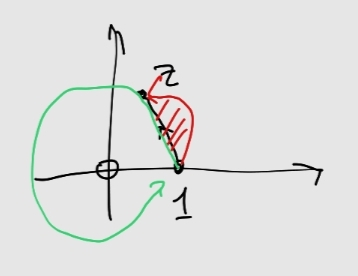
\includegraphics[scale=0.5]{fig2.jpg}
    \caption{A path going from $1$ to $z$ (black and red path). Another path from $1$ that encircles the origin (green path)}
\end{figure}
But the integral is undefined at the origin. To fix this, we draw a path from
$1$ that encircles the origin, and ends back at $1$ (green path).
This is one example of a Riemann surface(????).\\\\
As a second example, define the subset of $\C^2$, 
$$S = \lbrace (z,w)\in\C^2 : z = w^2\rbrace.$$
We can infer information about $\sqrt{z}$ by studying the structure of this 
space. \\\\
This leads us to the rigorous definition of a Riemann surface: which is a 
topological surface equipped with a complex structure.

\begin{example}
    Define $$w = \sqrt{(z^2-1)(z^2-k^2)},$$
    where $k \in \C$, and $z\neq \pm1,\pm k$.
    This is an elliptic curve, apparently. 
    Let us re-write this as 
    $$z^2 = (z^2-1)(z^2-k^2).$$
    What does this look like as a subset of $\C^2$?\\\\
    (Fig 3) As before, we fix some base points, in this case, $\pm 1,\pm k$,
    and draw some paths that avoid these points, and perform a path integral 
    --- in this case, the integral evaluates to zero (green path). \\\\
    If the path goes around one of those points (red path), say near $z=1$,
    then let $u=z-1$. Then, 
    $$w = \sqrt{u} \sqrt{(z+u)(1+k+u)(1-k+u)},$$
    and observe that the function inside the square root of the second 
    factor is holomorphic, and does not vanish at $u=0$. 
    Repeating this process for each point, and cutting along the paths
    in the figure below, and then gluing them together. 
    \begin{figure}[h!]
        \centering
        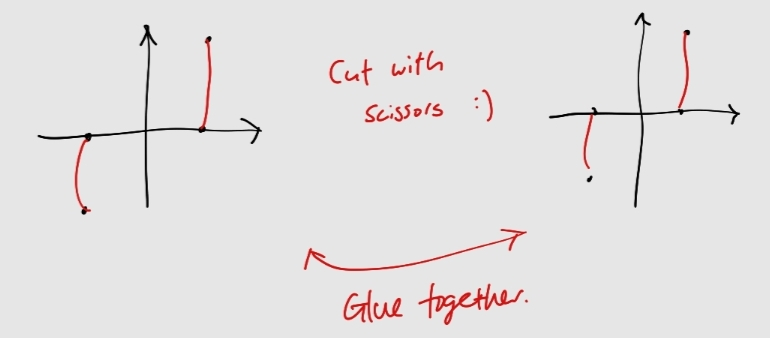
\includegraphics[scale=0.25]{fig4.jpg}
        \caption{Cutting along the paths of the points $z=\pm1,\pm k$.}
    \end{figure}
    The thing that you end up 
    getting from this construction is a torus with two points removed:
    \begin{figure}[h!]
        \centering
        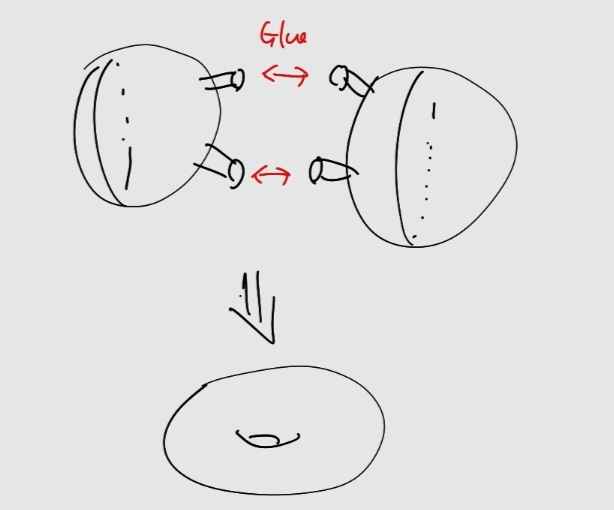
\includegraphics[scale=0.25]{fig5.jpg}
        \caption{Gluing the pieces together to make a torus with two 
        punctures.}
    \end{figure}
\end{example}

\subsection{Holomorphic Functions}

There are several definitions of what this means.

\begin{definition}
    \leavevmode
    \begin{itemize}
        \item[(a)] Let $D\subseteq \C$ be an open subset. Then, a function 
            $f : D \to \C$ is \emph{holomorphic} if $f$ is \emph{differentiable}
            (in the real sense), and moreover satisfies
            the \emph{Cauchy-Riemann equation}:
            $$i\frac{\partial f}{\partial x} - \frac{\partial f}{\partial y}=0.$$
            This definition identifies $\C$ with $\mathbb{R}^2$, and treats
            $f$ as a function on $\mathbb{R}^2$.
        \item[(a')] Alternatively, we can say that $f$ is \emph{holomorphic} 
            if the limit $$\lim_{h\to0} \frac{f(z+h)-f(z)}{h},$$
            exists for all $z\in \D$. This condition is equivalent to (a).
            \begin{remark}
                The Cauchy-Riemann equations is encoded in this definition
                in the following way:
                the limit definition implies that there exists some $M\in\C$ 
                such that $$f(z+h)-f(z) = Mh + O(h^2).$$
                Identifying $f : D\subseteq \mathbb{R}^2 \to \mathbb{R}^2$, 
                we get a $2\times 2$ matrix with real entries for the Jacobian
                $df$. Let $\lbrace 1,i\rbrace$ be a basis for $\C$.
                So, when does there exist some $M\in \C$ such that 
                $\C M \to \C$? To accomplish this, we write $i$ as a matrix,
                which gives us $$J = \begin{pmatrix}
                    0&-1\\
                    1&0
                \end{pmatrix}.$$
                Thus, there exists such an $M$ whenever $J(df) = df(J)$.
                From this, we may derive the Cauchy-Riemann relations.
                \begin{corollary}
                    If $f$ is holomorphic, then as a real function $f$ is 
                    smooth.
                \end{corollary}
                This leads to the next definition:
            \end{remark}
        \item[(a'')] $f$ is \emph{holomorphic} if $f$ is smooth and satisfies
            the Cauchy-Riemann equations. 
        \item[(b)] $f$ is \emph{holomorphic} if the Taylor expansion of $f$ 
            around each point $z\in D$ converges in a neighbourhood of $z$.
    \end{itemize}
\end{definition}

\textbf{Next Time:} More examples, and also will go through stuff to do with topological surface and complex structures.

\section{Lecture Two, 26/07/2023}

For Worksheet 2, WTS product of two holomorphic functions is holomorphic,
and addition of holomorphic functions is holomorphic. Second page of worksheet
is for later. 

\subsection{Definitions of Riemann Surface}

From last lecture, we know that a Riemann surface is a topological surface, 
equipped with a complex structure. We will define these two terms. 

\begin{remark}[Gufang Wisdom]
    When reading a research paper, focus on things you already know. When 
    going to lectures, focus on things that you don't know yet.
\end{remark}

Firstly, there is a notion of a topological manifold,
of a smooth/$C^\infty$ manifold, and a complex manifold. What these definitions
have in common is that one has to start with a topological space. \\\\
The first notion --- a topological manifold --- is a \emph{property} of a 
topological space. Whereas the second and third notions require some extra
structure.

\begin{definition}
    A topological space $X$ is a \emph{topological manifold} if:
    \begin{itemize}
        \item[(a)] locally Euclidean: for every point $x$, there exists an 
            open neighbourhood $U$ such that there is a homeomorphism 
            $U \to V \subseteq \mathbb{R}^n$.
        \item[(b)] it is Hausdorff: every two points can be contained in two 
            disjoint open neighbourhoods 
        \item[(c)] it is paracompact: there exists a basis of the topology that 
            consists of countably many open sets --- that is, it has a countable
            basis, or it is second countable 
    \end{itemize}
    If $n=2$, then $X$ is a \emph{topological surface}.
\end{definition}

One way to define a complex strucutre is to define a smooth or complex atlas.
Given one of those structures, the topological manifold becomes a smooth manifold
, respectively a complex manifold.\\\\
Recall that a smooth atlas is an open cover $\lbrace U_\alpha\rbrace$,
equipped with functions $\varphi_\alpha:U_\alpha\to\mathbb{R}^n$
such that each $\varphi_\alpha$ is a homeomorphic to its image, 
for all $\alpha,\beta$, the \emph{transition maps} $$\varphi_\alpha^{-1}\vert_{U_\alpha\cap U_\beta} \circ \varphi_\beta\vert_{U_\alpha \cap U_\beta}$$ is a diffeomorphism. 
A choice of smooth atlas gives a smooth structure on a topological manifold.
\begin{figure}[h!]
    \centering
    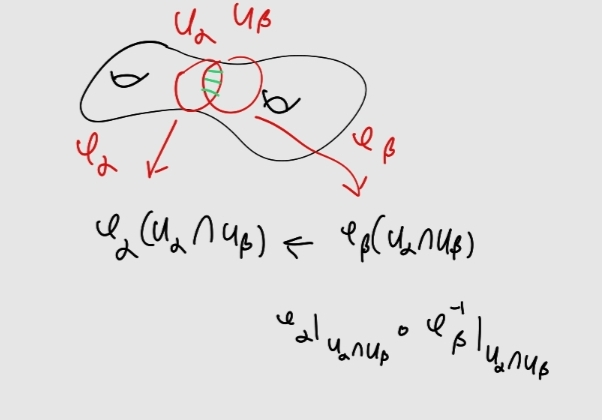
\includegraphics[scale=0.5]{fig6.jpg}
    \caption{Choice of smooth atlas on a manifold.}
\end{figure}
If we replace $\mathbb{R}^n$ with $\C^n$, and the word diffeomorphism 
with holomorphism, then we get a \emph{complex structure} on the 
topological manifold. 

\begin{lemma}
    Let $D$ and $D'$ be an open subset of $\C$, $f : D \to D'$ be a 
    holomorphic, bijective/invertible map. Then $f^{-1}$ is holomorphic.
\end{lemma}

\begin{definition}
    A function $f$ satisfying the property above is called \emph{biholomorphic}.
\end{definition}

\begin{definition}[Forster, Definition 1.1 - 1.3]
    Let $X$ be a two-dimensional manifold. A \emph{complex chart} on $X$ 
    is a holomorphism $\varphi : U \to V$, where $U\subseteq X$ and $V\subseteq\C$
    are open sets. Two complex charts $\varphi_i : U_i \to V_i$, for $i=1,2$
    are \emph{holomorphically compatible} if the map
    $$\varphi_2 \circ \varphi_1^{-1} : \varphi_1(U_1\cap U_2) \longrightarrow \varphi_2(U_1 \cap U_2),$$
    is biholomorphic. 
    A \emph{complex atlas} is a system of $\lbrace(U_\alpha,\varphi_\alpha)\rbrace$ of holomorphically compatible complex charts that cover $X$. Two complex
    atlases $\lbrace(U_\alpha,\varphi_\alpha)\rbrace$ and $\lbrace (V_\beta,\psi_\beta)\rbrace$ are \emph{analytically equivalent} if every chart of 
    $\lbrace (U_\alpha,\varphi_\alpha)\rbrace$ is holomorphically 
    compatible with every chart of $\lbrace(V_\beta,\psi_\beta)\rbrace$. 
    A \emph{complex strucutre} on $X$ is an equivalence class of analytically equivalent atlases on $X$.
\end{definition}

\begin{definition}[Forster, Definition 1.4]
    A \emph{Riemann surface} is a pair $(X,\Sigma)$, where 
    $X$ is a connected two-dimensional manifold, and $\Sigma$ is a complex 
    structure on $X$. 
\end{definition}

This is saying that the notion of a holomorphic function makes sense on 
open sets. This allows the definition of transition functions to make sense.
We will postpone the proof of this thing until later (maybe?).
Specifically, we wish to make sense of a complex atlas so that we can 
make sense of the following thing:

\begin{definition}
    Let $S$ and $S'$ be a topological surface, and $\lbrace U_\alpha\rbrace$,
    and $\lbrace V_\beta\rbrace$ atlases for $S$, and $S'$, respectively. 
    Then, a map $f: S \to S'$ is \emph{holomorphic} if for all $\alpha,\beta$,
    the map 
    $$(\varphi_\beta')^{-1} \circ f\vert_{U_\alpha \cap f^{-1}(V_\beta)} \circ \varphi_\alpha\vert_{U_\alpha\cap f^{-1}(V_\beta)}$$ is holomorphic.
    \begin{figure}[h!]
        \centering
        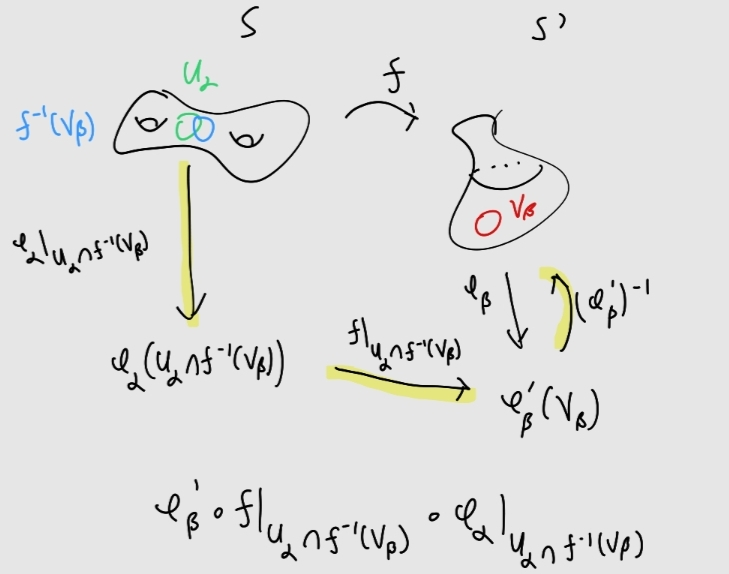
\includegraphics[scale=0.35]{fig7.jpg}
        \caption{Complex atlas on a Riemann surface. Highlighted arrows show 
            the compositions required to make the transition maps. Yes,
            the $\varphi_\beta'$ should be $(\varphi_\beta')^{-1}$ instead, but 
            I'm too lazy to fix it.}
    \end{figure}
\end{definition}

The whole point of giving a complex atlas is so that we can talk about 
complex manifolds that are not necessarily embedded within $\C^n$.

\begin{definition}
    Let $S$ be a topological surface, and $\lbrace U_\alpha\rbrace$,
    and $\lbrace U_\beta'\rbrace$ be two complex atlases on $S$.
    These two atlases are \emph{equivalent} if the identity map 
    $$\on{id}_S : (S,\lbrace U_\alpha\rbrace) \longrightarrow (S,\lbrace U_\beta'\rbrace),$$ is holomorphic. 
\end{definition}

We give a definition that is equivalent to the previous definition:

\begin{definition}
    A \emph{Riemann surface} is a pair $(S,\mcal{O}_S)$, where $S$ is a 
    topological surface, and $\mcal{O}_S$ is a sheaf of holomorphic functions on 
    $S$ --- called the \emph{structure sheaf} of $S$. \\\\
    In particular, for each open set $U \subseteq S$, we obtain a 
    $\C$-subalgebra $\mcal{O}(U)$ on $C^0(U)$ such that
    \begin{itemize}
        \item[(a)] For $V\subseteq U$ open sets in $S$, then 
            then the \emph{restriction map} 
            $r_U^V:\mcal{O}(U) \to \mcal{O}(V)$ 
            satisfies $r_U^V(\mcal{O}(U)) \subseteq \mcal{O}(V)$. 
        \item[(b)] (Locality/gluing) Given $\lbrace U_\alpha\rbrace$ an
            open cover of $S$, and given some $f \in C^0(U)$, if 
            $r_U^{U_\alpha}(f) \in \mcal{O}(U_\alpha)$, then $f\in\mcal{O}(U)$.
        \item[(c)] (Locally a disk) For all $x \in S$, there exists a 
            neighbourhood $U_x$ of $x$, and a homeomorphism 
            $\varphi_x: U_x \to \Delta$ ($\Delta$ is the unit disk), such that 
            there is a holomorphism 
            $-\circ\varphi_x : \mcal{O}(\Delta) \to \mcal{O}(U_x).$
    \end{itemize}
\end{definition}

Generally, the idea is that given an open cover $\lbrace U_\alpha\rbrace$,
we want to show that each $U_\alpha$ locally looks like a disk $\Delta$ intersect
with some open set. And since we know what it means for maps $f\vert_{U_\alpha}$
to be holomorphic, we can then make sense of holomorphic maps between surfaces.

\section{Lecture Three, 28/07/2023}

\paragraph{What is $\on{res}_{z=\infty}z$?} 
\paragraph{Answer:} Plug in $u = \frac{1}{z}$,
and we obtain $\on{res}_{u = 0} \frac{1}{u} = \on{res}_{u=0}u^{-1}= 1$.
But we can also take the derivative to obtain $\mathrm{d}z = -\frac{1}{u^2}\mathrm{d}u$, and so $$\on{res}_{u=0}\frac{1}{u} \left(-\frac{1}{u^2}\mathrm{d}u\right) = 0.$$
So, for this object we are going to avoid talking about residue of a function,
since composing functions together changes the value of the residue, as we
saw above.\\\\
To make sense of this, we first consider the Riemann sphere 
$\C \cup \lbrace\infty\rbrace = \mathbb{P}^1$. This is an example of a 
Riemann surface, with atlas given by stereographic projection. Then, the 
residue of the function above can be seen by composing the following functions 
(see figure 8, and the diagram you drew).\\\\
As a second example, let us now consider $\C$ equipped with a group
action $\mathbb{Z}\oplus \tau\mathbb{Z}$ (see figure 9). 
Taking the quotient $\C/(\mathbb{Z}\oplus \tau\mathbb{Z})$, we can then 
show that this is homeomorphic to a torus, whose complex structure is given 
by the lattice (see figure 10).

\begin{exercise}
    When do you have a holomorphic map from 
    $\C/(\mathbb{Z}\oplus \tau\mathbb{Z})$
    to the torus?
\end{exercise}

\subsection{$z = \sqrt{w}$}

Recall the example from day one given by $w(z) = \sqrt{z}$. The problem 
arises when one realises since for each $z$, there are two possible values for 
$w$. In particular, we have a subset of $\C^2$ given by:
$$S :=\lbrace (w,z) \in \C^2 : w^2 = z\rbrace,$$
which we claim is a Riemann surface, and further that there is 
a well-defined map (i.e. single-valued) function $S \to \C$, by replacing 
one of the variables with the other. But additionally,
we want this to be a holomorphic function.\\\\
Indeed, if $S$ has the structure of a Riemann surface, then it would make sense 
to talk about holomorphic functions from $S$. So, as a first step we will 
show that $S$ is a Riemann surface. Indeed, $S$ is a topological surface, 
so now we just need to construct an atlas on it.\\\\
First, we view $z$ as a function of $w$, and we get a function $f(w) = w^2$, 
which is holomorphic on $\C$. Then, the graph of the function $w$
is given by $w = f^{-1}(z)$.
Define a projection map $$p : S \to \C, \quad (z,w) \longmapsto w,$$
which is a homeomorphism since $S$ is the graph of a continuous function.
This gives a complex structure.

\begin{theorem}[Inverse Function Theorem]
    Suppose that $F : \C^2 \to \C$ is a holomorphic function with 
    $\frac{\partial F}{\partial w}(p) \neq 0$, and there 
    exists a neighbourhood $p \in U_1\times U_2 \subseteq\C^2$ and 
    $g : U_1\to U_2$ such that $F^{-1}$ exists on $S\cap U_1\times U_2$,
    where $S$ is the graph of $F$. The same happens when the partial 
    derivative of $F$ in the other variable is non-zero at $p$.
\end{theorem}

\subsection{Facts about Toplogical Surfaces}

\begin{theorem}
    Let $S$ be a topological surface. Then, if $S$ admits a complex atlas,
    then $S$ is orientable.
\end{theorem}

This implies that the determinant of a holomorphic function is always positive.

\begin{theorem}
    If $S$ is compact and orientable, then it is one of the following (figure 11).
    That is, compact surfaces are classified by their genus.
\end{theorem}



\chapter{Week Two}

\paragraph{This week, we learned \ldots}

\section{Lecture 1, 31/07/2023}

\subsection{Properties of Holomorphic Maps of Riemann Surfaces}

Recall that holomorphic functions can be defined in terms of a convergence 
of a Taylor series. 
But the convergence of the Taylor series is independent of the chart, despite
 the fact that the series depends on the choice of chart. 
 Consider a biholomorphic function $f : U\to V$, and a function $h : V \to \C$.
 Then, the composition $h\circ f$ is holomorphic.

 \begin{exercise}
    Let $U\subseteq S$ be an open subset of a Riemann surface $S$, and $V\subseteq S'$ an open subset of another Riemann surface $S'$. 
    Then, let $f : U\to V$ be a holomorphic function. 
    Then, given maps $\varphi : U \to \C$ and $\psi : V \to \C$,
    then we have a map $\psi \circ f \circ \varphi^{-1} : U \to V$,
    which is also holomorphic. Taking its Taylor expansion, we have:
    $$\psi \circ f \circ \varphi^{-1} = a_kz^k + a_{k+1}z^{k+1} + \cdots,$$
    where $a_k \neq 0$, and $k > 0$.  Show that $k$ is independent of $\psi$ and $\varphi$.
 \end{exercise}

 \begin{definition}
     The number $k$ from the exercise is called the ``valuation'' or the ``valencity'', and we denote it by $\nu_x(f) \in \mathbb{N}$, for some $x \in S$. 
 \end{definition}

\begin{theorem}
    Let $X$ and $Y$ be two Riemann surfaces, and $f: X \to Y$ a holomorphic, 
    non-constant map. Then, there exists an open set $U_x\subseteq X$ contaning
    a point $x$, and another open set $U_{f(x)} \subseteq Y$ 
    with charts $\varphi : U_x \to \C$ and $\varphi' :U_{f(x)} \to \C$. 
    Let $V = \varphi(U_x)$, and $V' = \varphi'(U_{f(x)})$. Then, for 
    every $x \in X$, and every such holomorphic map, there is a commutative 
    diagram given by:
    $$
    \begin{tikzcd}
a \arrow[d, maps to] & U_x \arrow[r, "f"] \arrow[d, "\varphi"] & U_{f(x)} \arrow[d, "\varphi'"] & f(a) \arrow[d, maps to] \\
0                    & V=\varphi(U_x) \arrow[r]                & V'=\varphi'(U_{f(x)})          & 0                       \\
                     & z \arrow[r, maps to]                    & z^k                            &
\end{tikzcd}
$$
What this is saying is that locally, transition maps are given by a 
function $f(z) = z^k$, where $k$ is the valuation at $x$. 
\end{theorem}

\begin{proof}[Idea of Proof]
    The proof of this can be found in Forster, Theorem 2.1.
    The idea is to start with any chart, and then write your function
    into the form $\psi \circ f\circ \psi^{-1} = z^k\cdot g(0)$,where 
    $g(0) \neq 0$. Then, we find that there exists some holomorphic function
    $h(z)$ such that $h(z)^k = g(z)$. It follows then that 
    $z\cdot h(z)$ is biholomorphic around a neighbourhood of $0$. 
    Call $\alpha(z) := z\cdot h(z)$. Then, $\alpha \circ g$ gives a 
    new chart. 
\end{proof}

\begin{theorem}[Forster, Theorem 2.1, ``Local Behaviour of Holomorphic Mappings]
    Let $X$ and $Y$ be Riemann surfaces, and $f: X\to Y$ a non-constant,
    holomorphic mapping. Let $x \in X$ and $y := f(x)$. Then, there exists 
    an integer $k\geq 1$ and charts $\varphi : U \to V$ on $X$ and 
    $\psi:U'\to V'$
    on $Y$ with the following properties:
    \begin{itemize}
        \item[(a)] $x\in U$, $\varphi(x) =0$, and $y\in Y$, $\psi(y) = 0$.
        \item[(b)] $f(U) \subseteq U'$. 
        \item[(c)] The map $F := \psi \circ f\circ \varphi^{-1} : V \to V'$
            is given by $z\mapsto z^k$.
    \end{itemize}
\end{theorem}

%\begin{proof}
%    (a) and (b) follow quickly by choosing a chart $\varphi_\alpha : U_\alpha\to V_\alpha$ on $X$ and $\psi : U'\to V'$ on $Y$ such that (a) and (b) are 
%    satisfied. It follows by the identity theorem [Forster, Theorem 1.11], that 
%    the function $$f_1 := \psi \circ f \circ \varphi_\alpha^{-1} : V_\alpha \to V'$$ is non-constant.
%\end{proof}

\begin{corollary}[Open Mapping Theorem]
    Let $f: X\to Y$ be a holomorphic, non-constant map. If $U\subseteq X$ 
    is open, then $f(U)$ is open. 
\end{corollary}

\begin{corollary}
    A bijective holomorphic function has a holomorphic inverse.
\end{corollary}

\begin{proof}
    Obvious\ldots? Injection so $k=1$.
\end{proof}

\begin{corollary}[Maximum Principal]
    Let $D\subseteq S$ be an open subset of a Riemann surface $S$, and 
    $D' \subseteq \C$ an open subset. Let $f : D \to D'$ be a holomorphic map,
    and $\vert f\vert$ has a local maximum at $s\in S$. Then, there 
    exists an open set $U\subseteq D$ such that $f\vert_U \equiv C$,
    for some constant $C$.
\end{corollary}

\begin{corollary}
    If $X$ is a compact, connected Riemann surface, and $Y$ 
    is a connected Riemann surface, and $f: X \to Y$ is a holomorphic, 
    non-constant map of Riemann surfaces, 
    then $f$ is surjective and $Y$ is also compact.
\end{corollary}

\begin{proof}
    Surjectivity of $f$ follows from open mapping theorem, and the fact that 
    the domain is compact and connected. Compactness of $Y$ follows from the fact
    that compactness is a topological invariant.
\end{proof}

\begin{corollary}
    If $X$ is a compact, connected Riemann surface, and $f : X \to \C$ 
    is a holomorphic function, then $f$ is constant. 
\end{corollary}

\begin{corollary}
    Let $f : X \to Y$ be a holomorphic non-constant map of Riemann surfaces.
    Let $$S := \lbrace x \in X : \nu_x(f) > 1\rbrace.$$
    Then, $S$ is an \emph{isolated subset} --- that is, at every point $s\in S$ 
    there  exists a neighbourhood of that point such that the only point in 
    $S$ is $s$ itself.
\end{corollary}

%\subsection{Homology Groups of Riemann Surfaces}
%
%$H_0$ and $H_2$ are straightforward if the Riemann surface is compact and 
%connected --- in this case they are both just isomorphic to $\mathbb{Z}$.


\begin{definition}
    Let $X$ and $Y$ be connected Riemann surfaces, and $f : X\to Y$ 
    a holomorphic, non-constant map. Then, for some $y \in Y$,
    the pre-image $f^{-1}(y) \subseteq X$. Then,
    the sum $$\deg f :=\sum_{r\in f^{-1}(y)} \nu_f(r),$$
    is the \emph{degree} of $f$.
\end{definition}

\begin{corollary}
    The degree of $f$ is independent of the choice of $y\in Y$.
\end{corollary}

\begin{proof}
    Exercise.
\end{proof}

\begin{example}
    Let $f(x)$ be a polynomial of degree $n$ over $\C$.
    Then, consider the set $\lbrace x \in \C : f(x) = a\rbrace$.
    It follows then that the number of solutions is always $n$ 
    by the fundamental theorem of algebra. It follows then that 
    $\deg f = n$. In light of this, one may view the degree of a 
    map of Riemann surfaces to be similar to this --- especially 
    since such maps are locally of the form $z\mapsto z^k$.
\end{example}

\begin{definition}
    A \emph{polygonal decomposition} of a topological surface is the following:
    \begin{itemize}
        \item[(a)] A set of isolated points $V$, called the \emph{vertices}
        \item[(b)] A set of continuous paths $\gamma: [0,1] \to S$ such that 
            the end points are in $V$, and homeomorphic on $(0,1)$ (so we don't get crossings in the path). Call this set $E$, the \emph{edges}.
        \item[(c)] Let $S\setminus E$ be the complement of all edges, and each
            connected component of $S\setminus E$ is called a \emph{face}.
        \item[(d)] 
            %$\bigcup_{r\in E} r([0,1])$. 
    \end{itemize}
\end{definition}

\begin{example}
    (see picture) two great circles of torus are edges (blue lines), and
    so there are two edges.
    The complement is given by cutting the tube open, and we get a square.
    We then see that $V+E-F = 0$.(TODO: make this a figure)
\end{example}

\begin{theorem}[Riemann-Hurewitz Formula]
    Let $f: X \to Y$ be a holomorphic, non-constant map of connected,
    compact Riemann surfaces. Then, $$\chi(X) = \deg(f) \cdot \chi(Y) - b,$$
    where $$b = \sum_{y \in Y} \sum_{x\in f^{-1}(y)} (\nu_f(x)-1).$$
    This constant $b$ is called the \emph{total ramification index}.
\end{theorem}

\section{Lecture 2, 02/08/2023}

Recall that we have introduced the notion of a ``valencity'' of a holomorphic 
map. This is a local notion --- in particular, it depends on some point $x$,
since it gives information about what happens in a neighbourhood of $x$. In 
particular, every holomorphic map is a two-to-one cover. \\\\
Recall that a covering space is a map $\pi : \mathfrak{S} \to S$ of topological 
surfaces such that for every $s \in S$, there is a neighbourhood $U$ of $s$
such that $\pi^{-1}(U) = \bigcup_d V_d$, and $\pi : U \to V_d$ is an isomorphism
for each $d$.
In particular, a map $z\mapsto z^2$ is a two-to-one cover.\\\\
More generally, $$\deg \pi = \vert \pi^{-1}(s)\vert,$$
where $\vert\cdot\vert$ denotes the cardinality. If both surfaces are compact,
then $\deg \pi$ is finite. 

\subsection{Branched Points and Branched Covers}
\begin{lemma}
    Suppose that $X$ is a compact Riemann surface, and $Y$ is a compact, connected
    Riemann surface, and $f : X \to Y$ a holomorphic mapping.
    Then, the set $S := \lbrace x \in X : \nu_x(f) \geq 2 \rbrace$ is finite.
\end{lemma}

Then, consider the set $Y\setminus f(S)$, and thus the map 
$X\setminus f^{-1}(f(S)) \to Y\setminus f(S)$. We then show that  
$f\vert^{Y\setminus f(S)}_{X\setminus f^{-1}(f(S))}$ is a covering map.
The set $S$ is the set of \emph{branched points}, and $f$ is a 
\emph{branched cover}.

\subsection{Meromorphic Functions}

\begin{definition}
    Let $U\subseteq S$ be an open, connected subset of a Riemann surface. 
    Then, a \emph{meromohphic function} on $U$ is a holomorphic
    map $f : U \to \mathbb{P}^1$ such that $f(U) \neq \lbrace \infty\rbrace$.
\end{definition}

\paragraph{How do you describe a holomorphic map $f : U \to \mathbb{P}^1$?} 
\paragraph{Answer:} Recall that $\mathbb{P}^1 = \C \cup \lbrace \infty\rbrace$ is the Riemann
sphere. We first have that $f^{-1}(\C) \subseteq U$. 
Let $V \subseteq f^{-1}(\C)$ be such that $f\vert_V : V \to \C$ 
is a holomorphic map. \\\\
Now, we wish to consider the complement of $V$. Let $z_0 \in U$ be such that 
$f : z_0 \mapsto \infty$. We require $f$ to be holomorphic around $\infty$, 
which means that there exists some neighbourhood $V_{z_0} \subseteq U$ of $z_0$ 
such that $f\vert_{V_{z_0}} = \frac{f_1}{f_2}$, whose numerator and denominator
are both holomorphic functions on $V_{z_0}$, $f_2(z_0) = 0$, and $f_1(z_0)\neq0$.

\begin{proposition}
    Let $f$ be a meromorphic function. Then, locally $f$ is of the form 
    $\frac{f_1}{f_2}$, with $f_2 \not\equiv 0$ --- that is, $f_2$ is not a 
    constant function $f_2 \equiv 0$, but it can still take the value of $0$
    at certain points.
\end{proposition}


\begin{definition}
    If $f(z_0) = \infty$, we say that $z_0$ is a \emph{pole} of $f$, and the 
    \emph{order} of the pole is the valencity $\nu_f(z_0)$. 
\end{definition}

\begin{example}
    Given the map $\C \to \mathbb{P}^1$ mapping $z\mapsto \frac{1}{z^2}$, 
    and $0\mapsto \infty$, we construct two charts to calculate the valencity.
\end{example}

Let $$\mcal{M}(S),$$ be the set of all meromorphic functions on $S$.

\begin{proposition}
    \begin{itemize}
        \item[(a)]
            $\mcal{M}(S)$ can be re-written to be the set:
            $$\mcal{M}(S) = \lbrace (f,V) : \text{$f : V \to \C$ is a holomorphic function, and the complement of $V$ is discrete}\rbrace/\simeq,$$
            where $(f_1,V_1) \simeq (f_2,V_2)$ if $f_1\vert_{V_1\cap V_2} = f_2\vert_{V_1\cap V_2}$.
        That is, one may view the algebra of meromorphic functions as germs of some kind?
        \item[(b)] $\mcal{M}(S)$ is a field.
    \end{itemize}
\end{proposition}

\begin{proof}
    \begin{itemize}
        \item[(b)] It is clear that $\mcal{M}(S)$ is a ring, so we wish to now 
            show that every meromorphic function has an inverse. This follows
            from the fact that we can always remove a discrete set of poles.
    \end{itemize}
\end{proof}

\begin{definition}
        Given $f \in \mcal{M}(S)$, then the \emph{zeroes} of $f$ 
        is is given by the elements of $f^{-1}(0)$, counted with multiplicity. The \emph{poles}
        of $f$ is the set $f^{-1}(\infty)$, counted with multiplicity. Denote
        these sets by $\mcal{Z}(f)$, and $\mcal{P}(f)$, respectively. 
        In particular, these are defined to be the formal linear 
        combination:
        $$\mcal{Z}(f) : = \sum_{z \in S, f(z) =0}\nu_f(0)z,$$
        and $$\mcal{P}(f) := \sum_{z\in S, f(z) = \infty}\nu_f(\infty)z.$$
\end{definition}

\begin{proposition}
    Let $S$ be a compact, connected Riemann surface, and 
    $f,g \in \mcal{M}(S)$ be non-constant functions. If $\mcal{Z}(f) = \mcal{Z}(g)$, and $\mcal{P}(f) = \mcal{P}(g)$, then $f = c\cdot g$, for some $c \in \C$.
\end{proposition}

\begin{proof}
    If $f/g$ has no poles, then the map $f/g : S \to \C$ is constant.
\end{proof}

\begin{example}
    Every mermomorphic function on $\mathbb{P}^1$ has a unique presentation 
    of the form: $$c\frac{\prod_{i=1}^m (z-z_i)}{\prod_{j=1}^n(z-p_j)}.$$
    In particular, it can be represented as a fraction of polynomials.
    Generally, any polynomial ringi $\C[z]$ is an integral domain, and thus has a field 
    of fractions. In this case, $\on{Frac}\C[z] = \C(z)$. All this shows is that 
    $$\mcal{M}(\mathbb{P}^1) = \C(z).$$
    Now, let us do the following construction: we adjoin $\C(z)$ by an 
    irreducible polynomial $w$, and 
    quotient out by an ideal $w^2=z$. Write this as 
    $$\C(z)[w] /(w^2 = z).$$
    Now, we have a finite extension of $\C(z)$, which is determined by $\C(z)$,
    and our choice of ideal that we quotient by. 
    Recall previously, that we took the set $\Sigma := \lbrace (z,w) : w^2 -z=0\rbrace$,
    from which we obtained a Riemann surface. The irreducibility of $w$ turns out
    to translate to the fact that $\Sigma$ is connected. From this, we may 
    construct $\mcal{M}(\Sigma)$. What this says is that finite field extensions
    of $\C(z)$ correspond to other meromorphic functions on Riemann surfaces.
\end{example}


\section{Lecture 3, 04/08/2023}

From complex analysis, there are three types of singularities: 
removable, isolated, and essential singularities. 
But for this course, we only focus on isolated singularities (or a pole). 
\subsection{$w(z) = \sqrt{z}$, again}
Let us come back to trying to define the function $w(z) = \sqrt{z}$, which is 
problematic because it's not actually a function. But algebraically, we never 
run into a problem since we can continually adjoining our field with 
square roots. We may view $z$ as a map $z : \C \to \C$, which we 
extend to $z: \C \to \mathbb{P}^1$, and view it as a meromorphic function 
on $\mathbb{P}^1$ --- $z\in \mcal{M}(\mathbb{P}^1)$. This corresponds
to a field extension of $\mcal{M}(\mathbb{P}^1)$. In particular, we adjoin
it by $\sqrt{w}$ to make a polynomial ring 
$\mcal{M}(\mathbb{P}^1)[\sqrt{w}]/(w^2-z=0)$, where 
$w^2-z$ is irreducible in $\mcal{M}(\mathbb{P}^1)[\sqrt{w}]$.\\\\
Let us consider the surface $$\pi : \Sigma = \lbrace (w,z) \in \C^2 : w^2-z = 0\rbrace \longrightarrow \C,\quad (w,z) \longmapsto z.$$
Using the same argument as before, this projection map equips $\Sigma$ with
a complex atlas --- the fact that the projection is a homemorphism follows 
from the fact that it is the graph of a holomorphic function $w^2 =z$.
Together, this gives $\Sigma$ the structure of a Riemann surface.
This tells us that the way we should think about $w(z)=\sqrt{z}$ as being 
not a function on $\C$, but rather as a pair $(\Sigma, f)$, 
where $f: \Sigma \to \C$ maps $(w,z)\mapsto w$ is a holomorphism. 
This is how we should think about this object geometrically.\\\\
We want a way to translate between the algebraic and geometric picture.
We know from last time that $\mcal{M}(\mathbb{P}^1) = \C(z)$, and here we have 
$\mcal{M} = \C(z)[\sqrt{w}]/(w^2-z=0)$.
In particular:
$$\lbrace \text{Irreducible polynomials over $F$}\rbrace \longleftrightarrow \lbrace (\mcal{M}(\Sigma),f) : \text{$f : \mcal{M}(\Sigma)\to \mcal{M}(\mathbb{P}^1)$ holomorphic}\rbrace$$

\begin{theorem}
    Finite extensions of a field of characterstic $0$ is primitive --- that is,
    generated by one element. 
\end{theorem}

\begin{theorem}[Theorem 8.9, Forster]
    Fix a connected Riemann surface $X$. Then, there is a one-to-one correspondence between irreducible polynomials $P(T) \in \mcal{M}(X)[T]$ and 
    pairs $(Y,f)$, where $\pi: Y \to X$ is a branched cover, and $f\in \mcal{M}(Y)$, such that the pullback
    $$\pi^\ast : \mcal{M}(X)[T] \longrightarrow \mcal{M}(Y)[T],$$
    has the property that $$(\pi^\ast P)(f)= 0.$$
\end{theorem}

\subsection{$\on{res}_{z=\infty}z = 0$ or $1$?}

Recall that one method is to do the Laurent expansion, and compute the 
coefficient from that. Alternatively, use the Cauchy integral formula:
$$a_{-1} = \frac{1}{2\pi i}\oint_C f(z)\mathrm{d}z,$$
where $C$ is a simple loop that encircles the point that we are taking
the residue of.\\\\
Let $\infty \in \mathbb{P}^1$, and consider a simple curve $C$ going around 
$\infty$ once. We then wish to project it down onto $\C$. 
It follows then by the Cauchy integral formula that 
$$\on{res}_{z=\infty} f(z) = \frac{1}{2\pi i}\oint_C f(z)\mathrm{d}z.$$
But by Green's theorem, this value is invariant under curve homotopies.
It follows then that $f$ is holomorphic in the interior of the curve, and 
it follows that $\on{res}_{z=\infty}f(z) = 0$. So, in order for Cauchy's formula to work, we have to ``force'' the residue to be $0$.

\subsection{$C^\infty$ Functions and Differential Forms}

We now wish to define smooth functions $f : U \to \C$, for some 
open subset $U\subseteq \C$. We may view $f$ as just a function in 
two variables. Recall that $f$ is holomorphic if the Cauchy-Riemann 
relations are satisfied. Viewing $f(x,y) = u(x,y) + iv(x,y)$, 
the Cauchy-Riemann equations may be written as 
$$\frac{\partial u}{\partial x} =\frac{\partial v}{\partial y},\quad \frac{\partial u}{\partial y} = -\frac{\partial v}{\partial x}.$$
More compactly, we may simply write it as $\overline{\partial f} = 0$. 
We may perform a change of basis from $x,y$ into variables 
$z,\overline{z}$ using the change of basis matrix 
$\begin{pmatrix}
    1&1\\
    1&-1
\end{pmatrix}$. Then, we may re-write the function as $f(z,\overline{z})$.
Then, 
$$\frac{\partial}{\partial\overline{z}} = \frac{\partial}{\partial x} -i\frac{\partial}{\partial y}.$$
Then, Cauchy-Riemann can be re-written to be 
$$\frac{\partial f}{\partial \overline{z}} = 0.$$
There is also $\partial f$, which is given by 
$$\frac{\partial f}{\partial z} = \frac{\partial}{\partial x} + i\frac{\partial}{\partial y}.$$

\begin{definition}
    Let $S$ be a topological surface, and $\lbrace (\varphi_\alpha, U_\alpha)\rbrace$ is a smooth atlas mapping $\varphi_\alpha:U_\alpha \to \mathbb{R}^2$. 
    A $C^\infty$ $0$-form is a smooth function on $S$. A $C^\infty$ $1$-form 
    is $\omega_\alpha= f_\alpha \mathrm{d}x_\alpha + g \mathrm{d}y_\alpha$
    such that on $U_\alpha \cap U_\beta$, 
%    $$\omega_\beta = f_\alpha \left(\frac{\partial x_\alpha}{\partial x_\beta}\mathrm{d}x_\beta + \frac{\partial x_\alpha{\partial x_\beta}\mathrm{d}y_\beta\right) + g_\alpha(\cdots).$$
\end{definition}

%\subsection{$(p,q)$-forms}
%
%Let $S$ be a topological surface, and $\lbrace U_\alpha\rbrace$ a 
%complex atlas on $S$, where $\varphi_\alpha U_\alpha \to \C(z_\alpha,\overline{z_\alpha})$. Then, $\varphi_\alpha \circ \varphi_\beta^{-1}$ being holomorphic
%means that $\frac{\partial z_\alpha}{\partial z_\beta} = 0.$
%
%\begin{definition}
%    $(p,q)$-forms. Read Forster.
%\end{definition}
%
%\begin{exercise}
%    These notions are independent of the choice of complex atlas.
%\end{exercise}

\chapter{Week Three}

\paragraph{This week, we learned about \ldots}

\section{Lecture 1, 07/08/2023}

\subsection{Review on Types of Singularities and Poles}

Let $a \in D \subseteq \C$ be a point in an open subset, and a holomorphic 
function $f : D\setminus \lbrace a\rbrace \to \C$. Then, 
$a$ is a \emph{removable singularity} if any one of the equivalent 
statements hold:
\begin{itemize}
    \item[(a)] if there exists $\widetilde{f} : D \to \C$ such that 
        $\widetilde{f}\vert_{D \setminus \lbrace a\rbrace} = f$,
    \item[(b)] There exists a continuous map $\widetilde{f}:D \to \C$ 
        such that $\widetilde{f}\vert_{D\setminus \lbrace a \rbrace} = f$,
    \item[(b')] $\lim_{z\to a}f(z)$ exists.
    \item[(c)] if $f$ is bounded in a punctured neighbourhood --- 
        that is, there exists some $a \in U \subseteq D$ such that 
        $f\vert_{U\setminus \lbrace a \rbrace}$ is bounded.
\end{itemize}

\begin{definition}
    Let $f$ be as above. Then, a point $a \in D$ is a \emph{pole} if 
    there exists $\widetilde{f} : D \to \mathbb{P}^1$ such that $\widetilde{f}$ 
    is holomorphic and $a \mapsto \infty$.\\\\
    Equivalently, $a\in D$ is a \emph{pole} if there exists 
    $\widetilde{f} : D \to \mathbb{P}^1$ a 
    continuous function such that $a \mapsto \infty$.
    Another way of saying this is that $a\in D$ is a pole if 
    $$\lim_{z\to a} \frac{1}{f(z)} = \infty.$$
    Or, $$\lim_{z\to a}\vert f(z) \vert = \infty.$$
\end{definition}

\begin{definition}
    A point $a \in D$ is an \emph{essential singularity} if 
    it is not removable, and not a pole. \\\\
    But this is not a useful definition. Instead, we can say that 
    $a \in D$ is an \emph{essential singularity} if the Laurent 
    expansion has infinitely many negative terms. Or, 
    neither the limit $\lim_{z\to a} f(z)$ nor $\lim_{z\to a}\frac{1}{f(z)}$
    exists. \\\\
    Alternatively, for all $a \in U \subseteq D$, the map 
    $f\vert_{U\setminus \lbrace a\rbrace} : U\setminus \lbrace a\rbrace\to \C$
    is $\infty$-to-$1$ for all values except possibly for one.
\end{definition}

\begin{proposition}
    Let $S$ be a compact Riemann surface, and 
    $$\mu(S) := \lbrace (f,V) :\text{$f : V \to \C$ is holomorphic}\rbrace/\simeq.$$
    Then, $V = S\setminus F$, where $F$ is discrete, and consists of 
    non-essential singularities. 
\end{proposition}

\begin{remark}
    $f$ is \emph{anti-holomorphic} if and only if $\overline{f}$ is
    holomorphic. Equivalently, 
    $$\frac{\partial}{\partial z}f = 0.$$ 
    We can also say that the composition of two antiholomorphic functions 
    is holomorphic. The composition of a holomorhpic function with 
    an anti-holomorphic one is holomorphic.
\end{remark}

\subsection{de Rham Cohomology and $(p,q)$-forms}

Let $S$ be a $C^\infty$ surface. Then, we obtain a notion of $C^\infty$
$n$-form on $S$, for $n=0,1,2$. Locally, these look like:
$$\mcal{E}_\alpha = f_\alpha \diff x_\alpha + f_\beta\diff x_\beta \in \mcal{E}^1(S),$$
and $$f_{\alpha\beta}\diff x_\alpha \wedge \diff x_\beta \in \mcal{E}^2(S).$$
There is a map 
$$\diff : \mcal{E}^0(S) \longrightarrow \mcal{E}^1(S), \quad f \longmapsto \diff f := \frac{\partial f}{\partial x_\alpha}\diff x_\alpha + \frac{\partial f}{\partial x_\beta}\diff x_\beta.$$
The fact that partial derivatives commute gives the fact that 
$\diff^2 = 0$.
Given a complex of differential forms:
$$0 \longrightarrow \mcal{E}^0(S) \longrightarrow \mcal{E}^1(S) \longrightarrow \mcal{E}^2(S) \longrightarrow 0,$$
the \emph{de Rham cohomology} is given by:
$$H_{\on{dR}}^0(S,\C) = \ker \diff_0,\quad H^1_{\on{dR}}(S,\C) = \frac{\ker \diff_1}{\on{Im} \diff_0}, \quad H^2_{\on{dR}}(S,\C) = \frac{\mcal{E}^2(S)}{\on{Im}\diff_1}.$$
Now, let us specify $S$ to be a Riemann surface. 
Then, $\mcal{A}^{0,0}(S)$ is the space of smooth $0$-forms on $S$.
Here, $\mcal{A}^{0,0}(S) = \mcal{E}^0(S)$. Let $\mcal{A}^{1,0}(S)$, and 
$\mcal{A}^{0,1}(S)$ be the space of $(1,0)$-forms and $(0,1)$-forms, respectively.
We have the property that $$\mcal{E}^1(S) = \mcal{A}^{0,1}(S)\oplus \mcal{A}^{1,0}(S).$$
Then, $\mcal{A}^{1,1}(S) = \mcal{E}^2(S)$, the space of $2$-forms. 
Observe that $$\ker\overline{\partial} = \mcal{O}(S) \subseteq C^\infty(S),$$
where we recall that $$\overline{\partial} f = \frac{\partial f}{\partial \overline{z_\alpha}} \diff \overline{z}_\alpha.$$
TODO: watch through this portion of the lecture again. I'm tired.

\section{Lecture 2, 09/08/2023}

Consider the category $\mathbf{SmthMflds}$ of smooth manifolds. 
Then, $C^\infty(-)$ defines a contravariant functor 
$$C^\infty(-) : \mathbf{SmthMflds} \longrightarrow \mathbf{Vect},\quad M \longmapsto C^\infty(M).$$
Similarly, one has a category $\mathbf{RieSurf}$ of Riemann surfaces.
The structure sheaf defines a functor:
$$\Gamma(-,\mcal{O}_S) : \mathbf{RieSurf} \longrightarrow \mathbf{Vect},\quad S \longmapsto\Gamma(S,\mcal{O}_S) := \mcal{O}_S(S),$$
called the \emph{global section functor}.



\subsection{Sheaves}

A \emph{pre-sheaf} $\mcal{F}$ of abelian groups on a topological space $X$ is a
contravariant functor
$$\mcal{F} : \mathbf{Open}(X) \longrightarrow \mathbf{AbGrp}, \quad U\longmapsto \mcal{F}(U).$$
Here $\mathbf{Open}(X)$ consists of open sets of $X$, and morphisms are
 given by inclusions. So, given two open subsets $U\subseteq V$, 
 with inclusion map $U\hookrightarrow V$, then the functor $\mcal{F}$
 induces a homomorphism of abelian groups: 
 $$r_U^V : \mcal{F}(V) \to \mcal{F}(U),$$
 the \emph{restriction map}.

 \begin{definition}
    A \emph{sheaf of abelian groups} is a pre-sheaf $\mcal{F}$ on a topological
    space $X$ such that:
    \begin{itemize}
        \item[(i)] (Locality) For an open cover $\lbrace U_\alpha\rbrace$ 
            of an open set $U$, then for all $f,g \in \mcal{F}(U)$,
            if $U\supseteq U_\alpha$, then there is a restriction map
            $r_{U_\alpha}^U : \mcal{F}(U) \to \mcal{F}(U_\alpha)$ mapping
            $f \mapsto f\vert_{U_\alpha}$, and $g \mapsto g\vert_{U_\alpha}$ 
            such that $f\vert_{U\alpha}=g\vert_{U_\alpha}$
            for all $\alpha$, then $f=g$.\\\\
            Equivalently, each restriction map 
            $\mcal{F}(U)\to\mcal{F}(U_\alpha)$ is injective.
        \item[(ii)] (Gluing) Given a collection $f_\alpha \in \mcal{F}(U_\alpha)$, 
            such that for all $\alpha,\beta$ such that $U_\alpha \supseteq U_\alpha \cap U_\beta$, 
            and restriction maps $r_{U_\alpha\cap U_\beta}^{U_\alpha}$ and $r_{U_\alpha \cap U_\beta}^{U_\beta}$ for which 
            $f_\alpha\vert_{U_\alpha \cap U_\beta}^{U_\alpha} = f_\beta\vert_{U_\alpha\cap U_\beta}^{U_\beta}$. Then, there exists $f\in \mcal{F}(U)$ such that
            $f_\alpha = f\vert_{U_\alpha}^U$.\\\\
            A homological reformulation of this condition can be given in the 
            following way. Consider the map:
            $$d^0 :\prod_\alpha \mcal{F}(U_\alpha) \longrightarrow \prod_{\alpha,\beta} \mcal{F}(U_\alpha\cap U_\beta), \quad (f_\alpha)\longmapsto (f_\alpha\vert_{U_\alpha\cap U_\beta}^{U_\alpha} - f_\beta\vert_{U_\alpha\cap U_\beta}^{U_\beta}).$$
            Then, the above discussion is equivalent to saying that 
            $\mcal{F}(U)$ surjects onto $\ker d_0$. 
            In fact, there is a short exact sequence of abelian groups:
            $$0 \longrightarrow \mcal{F}(U) \longrightarrow \prod_\alpha\mcal{F}(U_\alpha) \longrightarrow \prod_{\alpha,\beta}\mcal{F}(U_\alpha\cap U_\beta)\longrightarrow 0.$$
    \end{itemize}
 \end{definition}

 \begin{remark}
    Generally, one may replace ``abelian groups'' in the above definition
    with any category that you like. The category doesn't necessarily have
    to be abelian either --- for instance, $\mathbf{Ring}$ is not abelian,
    but we can still have a sheaf over it.
 \end{remark}

 \begin{example}
    Let $X$ be a topological space, and let $C^0$ be the 
    pre-sheaf of continuous functions sending $U\mapsto C^0(U)$.
    The restriction maps $C^0(U) \to C^0(V)$ are given by 
    just restricting  the function: $f\mapsto f\vert_V$.
    By definition, two functions are equal if they agree at each point,
    and the locality axiom is thus satisfied. Similarly, the gluing axiom
    follows from the fact that a function being well-defined means that 
    functions that are equal agree on intersections of open sets.
    It follows then that $C^0$ defines a sheaf of continuous functions on 
    $X$.
 \end{example}

 \begin{example}
    If $X$ is a smooth manifold, then $\mcal{E}^i$ 
    defines a pre-sheaf $U\mapsto \mcal{E}^i(U)$ giving smooth 
    $i$-forms on $U$. 
 \end{example}

 \begin{example}
    If $X$ is a Riemann surface, then similarly $\mcal{E}^{p,q}$ defines a
    pre-sheaf sending $U\mapsto \mcal{E}^{p,q}(U)$, which defines a
    $(p,q)$-form on $U$.
 \end{example}

 \begin{definition}
    A morphism of pre-sheaves $f: \mcal{F} \to \mcal{G}$ is a natural 
    transformation. 
 \end{definition}

\begin{definition}
    Let $\mcal{F}$ be a (pre)sheaf on $X$. 
    Then, a \emph{sub-(pre)sheaf} is a (pre)sheaf
    $\mcal{G}$ with a natural transformation $\mcal{G} \to \mcal{F}$ 
    such that for every open set $U$ of $X$, 
    $\mcal{G}(U) \to\mcal{F}(U)$ is injective.
\end{definition}

\begin{exercise}
    If $\mcal{F}$ is a sheaf of abelian groups on $X$, and 
    $\mcal{G}$ assigns $U\mapsto \mcal{G}(U)$, where $\mcal{G}(U)$ 
    is a subgroup of $\mcal{F}(U)$. Then, $\mcal{G}$ defines a 
    subsheaf of $\mcal{F}$ if for every open cover $\lbrace U_\alpha\rbrace$ 
    of $U$, then the diagram commutes:(TODO: put figure here)
    That is, 
    $\on{Im}(r_{U_\alpha}^U(\mcal{G}(U))) \subseteq \mcal{G}(U_\alpha)$.
\end{exercise}

\begin{corollary}
    Let $S$ be a Riemann surface. Then, $\mcal{O}_S$ is a subsheaf of $C^0$.
\end{corollary}

\begin{definition}
    Let $\mcal{F}$ be a sheaf on $X$, and $x \in X$.
    Then, the \emph{stalk of $\mcal{F}$ at $x$} is given by:
    $$\mcal{F}_x := \varprojlim_{x \in U}\mcal{F}(U) := \left\lbrace (f,U) : 
    \text{$U$ is a neighbourhood of $x$, and $f \in \mcal{F}(U)$}\right\rbrace/\sim,$$
    where $(f,U)\sim (g,V)$ if $f\vert_{U\cap V} = g\vert_{U\cap V}$, and the 
    limit runs over all open neighbourhoods of $x$.
\end{definition}

\begin{remark}
    If $\mcal{F}$ and $\mcal{G}$ are sheaves such that 
    $\mcal{F}_x \cong \mcal{G}_x$ for all $x \in X$, this does 
    \emph{not} imply that $\mcal{F} \cong \mcal{G}$!!
\end{remark}

\begin{example}
    Let $X$ be a connected topological space, and let 
    $\mathbf{Const}$ be the pre-sheaf mapping an open set $U$ 
    to constant $\C$-functions on $U$. This does not define a sheaf,
    since $U$ is not necessarily connected, and we run into issues
    where two constant functions can take two different values on an 
    intersection.\\\\
    However, if we replace constant with \emph{locally constant}, then we 
    can fix this issue. The sheaf resulting from this is called the 
    \emph{constant sheaf}.
\end{example}

\section{Lecture 3, 11/08/2023}

\subsection{More on Stalks of Sheaves}

Let $\mcal{F}$ be a sheaf on $X$. Given some open neighbourhood $U$ of 
$x \in X$, we obtain an abelian group $\mcal{F}(U)$. This gives an element
of the stalk $\mcal{F}_x$. In particular, there is an embedding 
$\rho_x : \mcal{F}(U) \hookrightarrow\mcal{F}_x$. A natural 
question to ask is how much information about the sheaf is embedded in the
$\mcal{F}_x$'s.

\begin{lemma}
    Let $\mcal{F}$ be a sheaf on a connected topological space $X$, and 
    $f \in \mcal{F}(U)$.
    Then, $f = 0$ if and only if $\rho_x : \mcal{F}(U) \to \mcal{F}_x$ 
    maps $f\mapsto \rho_x(f) = 0$ for all $x \in U$.
\end{lemma}

\begin{proof}
    Observe that $\rho_x(f) = 0$ if and only if there exists 
    some $x \in V \subseteq U$ open such that $f\vert_V = 0$.
    This is true for every other open neighbourhood $V_x \subseteq U$ of $x$, 
    and it follows by the locality property that $f=0$.
\end{proof}

\begin{definition}
    A sheaf $\mcal{F}$ on $X$ satisfies the \emph{identity theorem} if 
    for every open $U\subseteq X$, and for all $f \in \mcal{F}(U)$, 
    $f$ satisfies the property that 
    $f=0\in\mcal{F}(U)$ if there exists $x \in U$ such that 
    $\rho_x(f) = 0$ in $\mcal{F}_x$.
\end{definition}

The only difference between the above definition and the Lemma is that 
it is only sufficient to test $f$ on one element to determine that it is 
a zero section. What this tells us is that the stalk at a single point 
gives us information about what happens globally.

\begin{example}
    Let $S$ be a Riemann surface, and $\mcal{O}_S$ its structure sheaf.
    Given some open $x\in U\subseteq X$, we get a holomorphic function
    $f \in \mcal{O}_S(U)$. We wish to determine $\rho_x(f) \in \mcal{O}_{S,x}$.
    By the Lemma, this is saying that if $f = 0$, then 
    there is some open neighbourhood $V\subseteq U$ of $x$ such that 
    $f\vert_V = 0$, which thus implies that all derivatives of $f$ vanish.
\end{example}

\begin{example}[Non-example]
    Let $X$ be a smooth manifold, and $C^\infty_X$ a sheaf of 
    smooth functions on $X$. We show that this does not satisfy the 
    identity theorem --- that is, what happens at one point tells us nothing
    about what happens at another point.\\\\
    For every open $U\subseteq X$, and $x \in U$, there exists a smooth
    function on $X$ --- denoted by $\varphi \in C^\infty(X)$ --- such that 
    $\varphi(x) = 1$, and $\varphi\vert_{X\setminus U} = 0$, called the 
    \emph{bump function}. It is clear that since these functions exist,
    the sheaf $C^\infty_X$ does not satisfy the identity theorem.\\\\
    We recall them that we use these functions when talking about partitions
    of unity. What they show is how different sheaves of smooth functions
    are from sheaves of holomrophic functions.
\end{example}

\begin{theorem}[Partition of Unity]
    For all $\lbrace U_\alpha \rbrace$ an open cover of $X$, there exists 
    bump functions $\varphi_\alpha \in C^\infty(X)$ such that 
    $\varphi_\alpha \equiv 0$ on $X\setminus U_\alpha$, 
    and for all $x\in X$, there exists an open neighbourhood $x \in U_x\subseteq X$ such that $\varphi_\alpha\vert_{U_\alpha} \equiv 0$ for all 
    but finitely many $\alpha$'s.
\end{theorem}

What this is saying that, we can extend any local construction to a global
function. This is a unique feature of the smooth world.

\begin{definition}
    Let $f : \mcal{F} \to \mcal{G}$ be a morphism of sheaves. 
    We say that $f$ is \emph{surjective} if for all $x\in X$, 
    the maps $\mcal{F}_x\to\mcal{G}_x$ is surjective.
    We say that $\mcal{G}$ is a \emph{quotient sheaf} of $\mcal{F}$. 
\end{definition}

\begin{definition}
    A \emph{complex} of sheaves is a sequence of maps:
    $$\mcal{F}_0 \stackrel{d_0}{\longrightarrow} \mcal{F}_1\stackrel{d_1}{\longrightarrow} \mcal{F}_2 \longrightarrow\cdots.$$
    such that $d_{i+1}\circ d_i = 0$ for all $i$. We say that 
    the complex is \emph{exact at $\mcal{F}_1$} if for all $x\in X$,
    the sequence on the stalk $$\mcal{F}_{0,x} \stackrel{d_0}{\longrightarrow} \mcal{F}_{1,x}\stackrel{d_1}{\longrightarrow} \mcal{F}_{2,x},$$
    is exact.
\end{definition}

\begin{lemma}
    Let $f: \mcal{F} \to \mcal{G}$ be a morphism of sheaves.
    If, for every open neighbourhood $U$ of $x$, the map
    $\mcal{F}(U) \to \mcal{G}(U)$ is surjective, then 
    $\mcal{F}_x \to \mcal{G}_x$ is surjective.
\end{lemma}

\begin{proof}
    Use definition of stalk, and then take pre-image under 
    $\mcal{F}(U)\to\mcal{G}(U)$.
\end{proof}

\begin{remark}
    The converse is not true.
\end{remark}

\begin{example}
    Let $S$ be a Riemann surface. Associated to this we have 
    sheaves $\mcal{A}^{(0,0)}$, and $\mcal{A}^{(0,1)}$, and a 
    morphism of sheaves 
    $\overline{\partial} : \mcal{A}^{(0,0)} \to \mcal{A}^{(0,1)}$. 
    Recalling that a function (that is, a section of $\mcal{O}_S$) 
    is \emph{holomorphic} if $\overline{\partial}f = 0$. It follows
    then that the composition
    $$0\longrightarrow \mcal{O}_S \longrightarrow \mcal{A}^{(0,0)} \stackrel{\overline{\partial}}{\longrightarrow}\mcal{A}^{(0,1)}\longrightarrow 0,$$
    is exact --- that is, there is no cohomology at 
    $\mcal{A}^{(0,0)}$.
\end{example}

(TODO: watch this portion of lecture again)

\chapter{Week Four}

\paragraph{This week, we learned \ldots}

\section{Lecture 1, 14/08/2023}

Today, we have an entire hour of just examples

\subsection{An entire hour of examples}

\begin{example}
    \leavevmode
    \begin{itemize}
        \item[(a)] ($0$-th de Rham cohomology) Recall that given a Riemann surface $S$, we 
            have a de Rham complex given by:
            $$0\stackrel{d^{-1}}{\longrightarrow} \mcal{E}^0(S) \stackrel{d^0}{\longrightarrow} \mcal{E}^1(S) \stackrel{d^1}{\longrightarrow} \mcal{E}^2(S) \stackrel{d^2}{\longrightarrow} 0.$$
            Then, $$H_{\on{dR}}^i(S) := \frac{\ker d^i}{\on{Im}d^{i-1}}.$$
            In particular, $\ker d^i$ is the space of closed $i$-forms, and $\on{Im}d^{i-1}$ is the space 
            of exact $i$-forms.
            In particular, let us first calculate the $0$-th de Rham cohomology.
            Then, $$H^0_{\on{dR}} (S) = \ker d^0= \lbrace f\in C^\infty(S) : \diff f = 0\rbrace,$$
            which means that on $U_\alpha$, $$\frac{\partial f}{\partial z_\alpha}\diff z_\alpha = 0, \quad \frac{\partial f}{\partial z_\alpha}\diff \overline{z_\alpha}=0.$$
            It follows then that 
            $$H^0_{\on{dR}} = \lbrace \text{locally constant functions}\rbrace.$$
            If $S$ is connected, then $H^0_{\on{dR}}(S) = \C$.
            Otherwise, we have 
            $$H^0(S)_{\on{dR}} = \C^n,$$
            where $n$ is the number of connected components.
        \item[(b)] ($(0,0)$-th Dolbeaut cohomology) 
            We also have the double complex given by 
            $$0\longrightarrow \mcal{A}^{(0,0)}(S) \stackrel{\overline{\partial}}{\longrightarrow} \mcal{A}^{(0,1)}(S) \longrightarrow 0.$$
            The cohomology $H^{p,q}$ of this complex is then called 
            the \emph{Dolbeaut cohomology}.
            Here, $$H^{(0,0)}(S) = \ker\overline{\partial},\quad H^{(0,1)}(S) = \on{coker} \overline{\partial}.$$
            Let us compute the $(0,0)$-th cohomology of this object.
            Then, by definition
            $$H^{(0,0)}(S) = \lbrace \ker \overline{\partial}  =\lbrace f \in \mcal{A}^{(0,0)} : \overline{\partial}f=0\rbrace.$$
            That is, on every open set $U_\alpha$, 
            $$\frac{\partial f}{\partial \overline{z_\alpha}}\diff\overline{z_\alpha} = 0,$$
            which implies that 
            $$\frac{\partial f}{\partial \overline{z_\alpha}} = 0,$$
            which is precisely the definition of holomorphicity. It follows
            then that 
            $$H^{(0,0)}(S) = \mcal{O}_S.$$
        \item[(c)] ( $(1,0)$-th Dolbeaut cohomology) 
            $$H^{(1,0)}(S) = \ker\overline{\partial} = \lbrace \omega : \overline{\partial}\omega = 0\rbrace.$$
            So, we have on $U_\alpha$, 
            $$\frac{\partial g_\alpha}{\partial \overline{z_\alpha}} \diff\overline{z_\alpha}\wedge \diff z_\beta  =0,$$
            which implies that 
            $$\frac{\partial g_\alpha}{\partial \overline{z_\alpha}} = 0.$$
            It follows then that 
            $$H^{(1,0)}(S) = \Omega^1(S).$$
            If $S$ is not connected, then we can show that 
            $$\dim H^{(1,0)}(S) = g,$$
            the \emph{genus} of $S$.
        \item[(d)] ( $(0,1)$-th Dolbeaut cohomology)
            Let $\Delta$ be the unit disk, and let us try to compute 
            $H^{(0,1)}(\Delta)$. We recall a result from last time which 
            states that $\overline{\partial}$ is surjective on the unit disk.
            It follows then that 
            $$H^{(0,1)}(\Delta) = \on{coker}\overline{\partial} = 0.$$
    \end{itemize}
\end{example}

\begin{proposition}
    Let $S$ be a compact Riemann surface. Then,
    there is an injective vector space homomorphism of 
    $\Omega^1(S) = H^{(1,0)}(S)$ into $H^1_{\on{dR}}(S) = \ker d^1/\on{Im}d^0$.
\end{proposition}

\begin{proof}
    Let $\omega$ be a $(1,0)$-form --- that is, $\omega = g_\alpha\diff z_\alpha$.
    Then, it follows then that $\overline{\partial} \omega = 0$.
    That is, $$\frac{\partial f}{\partial \overline{z_\alpha}}\diff \overline{z_\alpha} = 0,$$
    which implies then that $\frac{\partial f}{\partial \overline{z_\alpha}}=0$.
    Then, it follows that $$\diff \omega = \frac{\partial f}{\partial \overline{z_\alpha}} \diff \overline{z_\alpha}\wedge \diff z_\beta + \underbrace{\frac{\partial f}{\partial z_\beta}\diff z_\beta \wedge \diff \overline{z_\alpha}}_{=0}=0,$$
    and it thus follows that the map indeed maps into $\ker d^1$.
    Let us try to show injectivity. Consider the 
    intersection $\Omega^1(S) \cap \on{Im}d^0$. 
    (TODO: watch the proof of this thing again)
\end{proof}

Together, we then have maps:
$$% https://tikzcd.yichuanshen.de/#N4Igdg9gJgpgziAXAbVABwnAlgFyxMJZARgBoAGAXVJADcBDAGwFcYkQAdDgW3pwAsAxk2ABBAL4A9YAAoy5AJTiZAZQUhxpdJlz5CKAEwVqdJq3ZduwxmKmyyxJavWbt2PASIOTDFm0ScPNbAAKJSxM4aWiAY7npE5KTEPmb+gVYiYZLkka4xOh76yEbJNL7mAZbBWQa5JjBQAObwRKAAZgBOENxIiSA4EEhkpn4WHBC0MB2MWGAwwFxo9B14TOJR7V09iH0DSEb99FiM7PwQEADWGyCd3UgAzDR7iAflaVDZ17fbB88ALGVUuwPsQvlshk9BogASAZnNgRBmAAjRhsGj8GD0KDsSDwp5HE4BXFscSUcRAA
\begin{tikzcd}
                               & {\mathcal{A}^{(1,0)}(S)} \arrow[r, "\overline{\partial}"] \arrow[d, hook] & {\mcal{A}^{(1,1)}(S)} \arrow[d, no head, equal] \\
\mcal{E}^0(S) \arrow[r, "d^0"] & \mcal{E}^1(S) \arrow[r, "d^1"]                                            & \mcal{E}^2(S)                                       
\end{tikzcd}$$

\begin{example}
    Let $S$ be some non-compact Riemann surface. In particular, let us take 
    $S = \C^\times$. Then, there is a map 
    $$\Omega^1(S) \longrightarrow H^1_{\on{dR}}(S),$$
    which we wish to describe. Further, we wish to describe $\Omega^1(S)$.
    We have maps:
    $$\begin{tikzcd}
    0 \arrow[r] \arrow[d]                                         & {\mcal{A}^{(1,0)}(S)} \arrow[r] \arrow[d] & {\mcal{A}^{(1,1)}(S)} \arrow[d, no head, equal] \\
    \mcal{E}^0(S) \arrow[r, "d^0"] \arrow[d, no head, equal] & \mcal{E}^1(S) \arrow[r, "d^1"] \arrow[d]  & \mcal{E}^2(S)                                        \\
    \mcal{E}^0(S) \arrow[r]                                       & {\mcal{A}^{(0,1)}(S)}                     &
    \end{tikzcd}$$
    \paragraph{Claim:} For all $g\diff \overline{z} \in \mcal{A}^{(0,1)}(S)$ such that 
    there exists $h\in C^\infty(S)$ such that $\diff h = g \diff\overline{z} + m\diff z \in \mcal{A}^{(1,1)}(S).$ \\\\
    Here $d^0 : h \mapsto \diff h$.
    The claim shows that the map $\mcal{E}^0(S) \to \mcal{A}^{(0,1)}(S)$ 
    is surjective. From this, it then follows that $\Omega^1(S) \cong H^1_{\on{dR}}(S)$.
    The fact that the claim implies this surjectivity is left as an exercise.
    \begin{proof}[Proof of Claim]
        Let $\lbrace U_\alpha\rbrace$ be an open cover of $S$ by disks
        $U_\alpha \cong \Delta$. Then, on each $U_\alpha$, there 
        exists some $h_\alpha \in C^\infty(U_\alpha)$ such that 
        $$\overline{\partial}h_\alpha = g\diff z\vert_{U_\alpha}.$$
        On $U_\alpha \cap U_\beta$, the function 
        $h_\alpha - h_\beta\vert_{U_\alpha \cap U_\beta}$ has the property that 
        $$\overline{\partial}(h_\alpha - h_\beta ) = 0.$$
        That is, $h_\alpha - h_\beta$ is a holomorphic function on 
        $U_\alpha \cap U_\beta$. We first require a lemma:
        \begin{lemma}
            There exists $H_\alpha \in \mcal{O}(U_\alpha)$  such that
            $H_\alpha - H_\beta = h_\alpha - h_\beta$ on $U_\alpha\cap U_\beta$.
        \end{lemma}
        This Lemma requires on the fact that $S=\C^\times$ is non-compact.
        We will prove this later, but for now we will simply use it.
        Let $h := h_\alpha-h_\beta$, and we observe that this function 
        is defined on each $U_\alpha$, and agree on the intersection
        $U_\alpha\cap U_\beta$. It follows then that 
        $h \in C^\infty(S)$. Computing its differential directly, we have:
        $$\diff h = \underbrace{\frac{\partial h}{\partial \overline{z}} \diff \overline{z}}_{=g\diff\overline{z}} + \frac{\partial h}{\partial z}\diff z,$$
        and thus we have proved the claim.
    \end{proof}
\end{example}

\section{Lecture 2, 16/08/2023}

\subsection{Homology of Riemann Surfaces}

Recall the definition of a polygonal decomposition. 
We have a finite set of vertices $V$, edges $E$ (non-self intersecting curves$\gamma : [0,1]\to $, except possibly at end points).
(look at picture on phone), and faces $F$.\\\\
We have a \emph{cellular chain complex} given by 
$$0\longrightarrow C_2 \stackrel{\delta}{\longrightarrow} C_1 \stackrel{\delta}{\longrightarrow} C_1 \stackrel{\delta}{\longrightarrow} C_0 \longrightarrow0,$$
where each cell is given by the $\mathbb{Z}$-span of the faces, edges, and 
vertices, respectively. 
The mapping goes $$\text{face $f$} \longmapsto \text{boundary of $f$, $\gamma$} \longmapsto \gamma(1) - \gamma(0).$$
(see picture on board)
In the case of the torus, this is given by 
$$\mathbb{Z} \longrightarrow \mathbb{Z}^2 \longrightarrow \mathbb{Z}, \quad f\longmapsto \gamma_1-\gamma_2-\gamma_1+\gamma_2 \longmapsto \gamma_1(1)-\gamma_1(0) = V- V = 0.$$
Generally, the \emph{cellular homology} of $S$ is given by:
$$H_i(S) := \frac{\ker \delta_i}{\on{Im}\delta_{i+1}},$$
where $\ker\delta_i$ is the \emph{group of $i$-cycles}, and $\on{Im}\delta^{i+1}$ is the \emph{group of $i$-boundary.}

\begin{lemma}
    Any closed curve $\gamma$ on $S$ is homotopic to a chain of edges.
    Moreover, $\gamma$ is a $1$-cycle.
\end{lemma}

(see picture with red curve on torus for exmaple of closed curve homtopic to
each other)
Now, let us fix a smooth $2$-manifold $S$, and a smooth atlas given by 
$\lbrace U_\alpha\rbrace$. Then, there exists a notion of piecewise smooth
curves $\gamma : [0,1]\to S$. Technically, we wish to think of smooth curves,
but for technical reasons to do with homotopy groups we want to think of 
piecewise curves.

\begin{lemma}
    Any continuous curve $\gamma : [0,1]\to S$ is homotopic to a piecewise
    smooth curve. Further, the homotopy preserves the boundary --- that is,
    given two curves $\gamma, \gamma' : [0,1]\to S$ and a homotopy
    $H :[0,1]\times [0,1] \to S$ such that 
    $H(0,-) = \gamma$ and $H(1,-)=\gamma'$ such that $H(-,0) = \gamma(0)=\gamma'(0)$, and $H(-,1)=\gamma(1)=\gamma'(1)$.
\end{lemma}

\subsection{Integrating Differential Forms}

Recall that  a $1$-form $\omega \in \mcal{E}^1(S)$ is locally, that is, 
on a chart $\varphi: U_\alpha \to \mathbb{R}^2$, $\omega$ looks like
$\omega_\alpha = f_\alpha\diff x_\alpha + g_\alpha \diff y_\alpha$.
Let $\gamma$ be a piecewise constant curve in $U_\alpha$. Then,
$$\int_\gamma \omega = \int_0^1 \left(f_\alpha(\gamma(t)) \frac{\diff x_\alpha}{\diff t}\diff t + g_\alpha(\gamma(t)) \frac{\diff y_\alpha}{\diff t}\diff t\right)\in \C.$$

\begin{proposition}
    \begin{itemize}
        \item[(a)] The value of the integral is independent of the chart
        \item[(b)] The value of the integral is independent of the 
            parametrisation of $\gamma$ --- it only depends on the orientation --- in particular, the curves must all go in the same direction.
        \item[(c)] (Fundamental Theorem of Calculus) 
            If $\gamma$ is a closed curve, then the integral only 
            depends on $\omega$ up to exact $1$-forms. That is, 
            $\int_\gamma \omega = \int_\gamma\omega +\diff \alpha$, for
            $\diff\alpha$ an exact $1$-form.
    \end{itemize}
\end{proposition}

\begin{example}
    Let $\C$ be acted upon by a lattice $\Lambda = \mathbb{Z}\oplus \tau\mathbb{Z}$, where the action is given by 
    $\lambda \cdot z = (1+\tau)\cdot (x+iy) = (x+1) + i(y+\tau)$.
    Then, let us consider a Riemann surface given by 
    $$S := \C/\Lambda.$$
    Let $\gamma_1$, $\gamma_2$ be curves going in the $1$ and $\tau$ 
    directions on the lattice, respectively. Choose a $1$-form given by 
    $\omega = \diff z$. By the $\Lambda$-invariance, 
    $$\diff (z+\tau) = \diff z,$$
    and it thus follows that this is a $1$-form on the quotient. The same 
    follows for the $1$ direction on the lattice. Now, let us try to integrate
    it. Computing, 
    $$\int_{\gamma_1} \diff z = 1.$$
    Similarly, 
    $$\int_{\gamma_2} \diff z = \tau.$$
    This looks like we are integrating a constant one-form on a closed loop, 
    but getting a non-zero number, which is weird. However, the idea 
    of a constant $1$-form does not make sense on a Riemann surface, which is 
    why we are getting this behaviour. 
\end{example}

\begin{corollary}
    The integral defines a pairing 
    $$\int : H_1(S,\mathbb{Z}) \times H^1_{\on{dR}}(S) \longrightarrow \C.$$
\end{corollary}

From the above example, $\gamma_1,\gamma_2$ are homology classes 
in $H_1(S,\mathbb{Z})$.
Let us see more facts about smooth curves on manifolds.

\begin{lemma}
    If $S$ is compact and orientable, then any two piece-wise smooth curves 
    $\gamma_1$, $\gamma_2$ (up to homotopy if necessary):
    \begin{itemize}
        \item[(a)] intersect at only finitely many smooth points
        \item[(b)] their intersection is transversal at each point --- 
            that is the tangent space of the two curves at each of the 
            intersections span a two-dimensional vector space
    \end{itemize}
    Let $p$ a point in the intersection of the curves --- written 
    $p \in \gamma_1\cap \gamma_2$. We define the 
    \emph{sign} of $p$ by:
    $$\on{sgn} (p) = \begin{cases}
        \text{$1$, if $T_p\gamma_1 \times T_p\gamma_2$ have positive orientation}\\
        \text{$-1$ if $T_p\gamma_1$ and $T_p\gamma_2$ have opposite orientations}
    \end{cases},$$
    where by $T_p\gamma_1 \times T_p\gamma_2$ we mean the cross product.
\end{lemma}

\begin{definition}
    If $\gamma,\eta$ are closed curves, then 
    $$\gamma \# \eta = \sum_{p \in \gamma \cap \eta} \on{sgn}(p)\in\mathbb{Z}.$$
\end{definition}

\begin{proposition}
    Let $S$ be a compact oriented Riemann surface. Then,
    \begin{itemize}
        \item[(a)] $\gamma \#\eta$ is invariant under smooth homotopies of 
            $\gamma$ and $\eta$.
        \item[(b)] If $\beta = \delta f$, where $f$ is a face, then 
            $$\beta\#\alpha = 0,$$ for all $1$-cycles $\gamma$. 
            In particular, the $\#$ operator is a well-defined, skew-symmetric
            non-degenerate bilinear form:
            $$\# : H_1(S,\mathbb{Z}) \times H_1(S,\mathbb{Z}) \longrightarrow \mathbb{Z}.$$
    \end{itemize}
\end{proposition}

\begin{example}
    (look at picture on phone of genus $2$  surface.)
    Consider a genus $2$ surface with faces 
    $a_1,a_2,b_1,b_2$, and their inverses. Under this bilinear form $\#$, 
    we get the following matrix given by the basis:
     $\begin{pmatrix}
        0&I\\
        -I&0
    \end{pmatrix}$
    In particular, this is the matrix representation of the bilinear form
     $\#$.
\end{example}

\section{Lecture 3, 18/08/2023 TODO: WATCH}

\chapter{Week Five}

\paragraph{This week, we learned \ldots}

\section{Lecture 1, 21/08/2023}

Let $\mcal{A}$ be an abelian category, and $f: a \to b$ a morphism in 
$\mcal{A}$. By definition, a cokernel object in $\mcal{A}$ is an object
$\on{coker} f$ such that in the diagram:
$$\begin{tikzcd}
a \arrow[r, "f"] \arrow[rd, "0"] & b \arrow[d, "f"] \\
                                 & \on{coker}f     
\end{tikzcd}$$
we have that 
\begin{itemize}
    \item[(i)] the diagram commutes: $p\circ f= 0$
    \item[(ii)] If $q : b \to c$, then there exists a unique map 
        $\on{coker} f \to c$.
\end{itemize}

\begin{example}
    Let $\mcal{F}$ and $\mcal{G}$ be sheaves of abelian groups on $X$. Then, 
    the map $f : \mcal{F} \to \mcal{G}$ lives in the categories
    $\mathbf{PreSh}(X)$ and $\mathbf{Sh}(X)$.
    We now define the cokernel object. For some open set $U$ in $X$, 
    define $$\mcal{F}(U) \stackrel{f}{\longrightarrow}\mcal{G}(U) \longrightarrow \on{coker}f(U)=:\on{coker}(f(U)),$$
    and thus we see that we should define the cokernel object to be the 
    the presheaf $U\mapsto \on{coker}f(U)$. 
    Indeed, it is immediate that this satisfies the conditions required to 
    be a cokernel in $\mathbf{PreSh}(X)$. 
\end{example}

\begin{example}
    There is an embedding $$\underline{\mathbb{Z}} \longrightarrow \underline{\mcal{O}},$$
    where $\underline{\mathbb{Z}}$ is the constant sheaf, and 
    $\underline{\mcal{O}}$ be the sheaf of locally constant functions.
    Then, one may show that the cokernel of this map is not a sheaf.
\end{example}

We recall that given an exact sequence 
$$\mcal{F} \longrightarrow \mcal{G} \longrightarrow \mcal{H}\longrightarrow 0,$$
of sheaves, we have that for all $x\in X$, there is a corresponding exact
sequence on the stalks 
$$\mcal{F}_x \longrightarrow \mcal{G}_x \longrightarrow \mcal{H}_x \longrightarrow 0.$$

\subsection{Exact Functors}

Let $\mcal{A}$ and $\mcal{B}$ be two abelian categories, and $F : \mcal{A}\to\mcal{B}$ be an abelian functor (that is, the abelian-ness of the hom-sets are preserved under $F$). Then, we say that $F$ is \emph{exact} if 
for all short exact sequences $0\to a \to b \to c \to 0$ in $\mcal{A}$, 
$0\to F(a) \to F(b) \to F(c) \to 0$ is exact in $F(\mcal{B})$. \\\\
We say that $F$ is \emph{left exact} if for all exact sequences $0\to a \to b \to c$, then $0 \to F(a) \to F(b) \to F(c)$ is exact. 
The thing to be careful here is that the map $F(b) \to F(c)$ may not be 
exact.

\begin{example}
    The functor $\mathbf{Sh}(X) \to \mathbf{PreSh}(X)$ is left exact, 
    but not exact. That is, the cokernel in $\mathbf{Sh}(X)$ is not 
    necessarily the cokernel of $\mathbf{PreSh}(X)$ under the image 
    of this functor.
\end{example}

The functor that we will be most interested in working with is the global 
section functor 
$$\Gamma(X,-) : \mathbf{Sh}(X) \longrightarrow \mathbf{AbGrps},\quad \mcal{F} \longmapsto \Gamma(X,\mcal{F}).$$
Once again, this is only left exact, it is not exact. 

\begin{example}
    Let $A \in \mcal{A}$, where $\mcal{A}$ is an abelian category.
    Then, $\on{Hom}_\mcal{A}$ defines a functor
    $$\on{Hom}_\mcal{A}(A,-) : \mcal{A} \longrightarrow \mathbf{AbGrps},\quad B \longmapsto \on{Hom}_\mcal{A}(A,B).$$
    This is a covariant functor that is left exact but not exact.
    $\on{Hom}_\mcal{A}(-,B)$ is a contravariant functor. Once again, this 
    is left exact, but not exact.
\end{example}

\begin{exercise}
    The global sections functor $\Gamma(X,-) : \mathbf{Sh}(X) \to \mathbf{AbGrps}$, is the same as the functor $\on{Hom}_{\mathbf{Sh}(X)}(\underline{\mathbb{Z}},-)$.
\end{exercise}

\subsection{Injective Objects}

\begin{definition}
    An object $I \in \on{Obj}\mcal{A}$ is \emph{injective} if 
    $\on{Hom}_\mcal{A}(-,I)$ is exact.
\end{definition}

The idea is to start with any left-exact functor $F:\mcal{A} \to \mcal{B}$.
Then, for any short exact sequence $0\to a \to b \to c \to 0$ in $\mcal{A}$,
we have that $0 \to F(a) \to F(b) \to F(c)$ in $\mcal{B}$. We wish to
measure the extent to which the map $F(b) \to F(c)$ is non-surjective.
The natural way to capture this is using the cokernel --- specifically 
$\on{coker}(F(b) \to F(c))$.\\\\
In particular, we want a systematic way of ``filling up'' this sequence 
to the right, so that we can make it exact.

\begin{definition}
    Let $\mcal{A}$ be an abelian category, and $\mcal{C}$ a collection 
    of objects in $\mcal{A}$. Then, a \emph{$\mcal{C}$-resolution} --- 
    or, a resolution by objects in $\mcal{C}$ --- is a pair 
    $(\mcal{C}^\ast, a \to \mcal{C}^\ast)$, where 
    $$\mcal{C}^\ast = \mcal{C}^0 \to \mcal{C}^1 \to \cdots,$$
    with $\mcal{C}^i \in \mcal{C}$ and 
    $$0 \longrightarrow a \longrightarrow \mcal{C}^0 \longrightarrow \mcal{C}^1 \longrightarrow \cdots,$$
    is exact.
\end{definition}

\begin{example}
    Let $\mcal{I}$ be the collection of all injective objects in an abelian
    category $\mcal{A}$. Then, a resolution of objects in $\mcal{I}$ 
    is called an \emph{injective resolution}.
\end{example}

\begin{definition}
    An abelian category $\mcal{A}$ has \emph{enough injectives} if every 
    object admits an injective resolution.
\end{definition}

\begin{exercise}[Horseshoe Lemma]
    If $\mcal{A}$ is an abelian category such that every object has an 
    injective resolution, with an exact sequence $0\to a \to b \to c\to 0$,
    then there exist injective resolutions $\mcal{I}^\ast(a)$, $\mcal{I}^\ast(b)$, 
    $\mcal{I}^\ast(c)$, such that 
    $$0 \longrightarrow \mcal{I}^\ast(a) \longrightarrow \mcal{I}^\ast(b) \longrightarrow \mcal{I}^\ast(c) \longrightarrow 0,$$
    such that these maps commutes with the differentials in the complexes
    $\mcal{I}^\ast(-)$, for $-=a,b,c$.
\end{exercise}

\begin{corollary}
    Let $F = \on{Hom}_\mcal{A}(b,-)$, and $\mcal{A}$ be an abelian 
    category with enough injectives.
    Then, we obtain a short exact sequence:
    $$0 \longrightarrow F(\mcal{I}^\ast(a)) \longrightarrow F(\mcal{I}^\ast(b)) \longrightarrow F(\mcal{I}^\ast(c)) \longrightarrow 0,$$
    which extends to a long exact sequence by the Snake lemma.
\end{corollary}

\begin{definition}
    Let $\mcal{A}$ be an abelian category with enough injectives.
    The \emph{right derived functor} of a functor $F$ is given by 
    $$R^iF(a) := H^i\left( F(\mcal{I}^\ast(a)\right).$$
\end{definition}

\begin{corollary}
    \leavevmode
    \begin{itemize}
        \item[(a)] If $0 \to a \to b \to c \to 0$, then there is a long 
            exact sequence 
            $$\cdots \longrightarrow R^iF(a) \longrightarrow R^iF(b) \longrightarrow R^iF(c) \longrightarrow R^{i+1}F(a) \longrightarrow \cdots$$
        \item[(b)] Each $R^iF(-)$ is independent of the choice of injective 
            resolution.
    \end{itemize}
\end{corollary}

\paragraph{Goal for this week:} Calculate $$H^i(X,-) := R^i\Gamma(X,-) : \mathbf{Sh}(X) \longrightarrow \mathbf{AbGrps},$$
called the \emph{sheaf cohomology} of $X$.
\begin{remark}
    The domain of these functors is technically in the \emph{derived category}
    of $\mathbf{Sh}(X)$.
\end{remark}
There is a special collection of objects in $\mathbf{Sh}(X)$ in $\mathbf{Sh}(X)$
called \emph{flasque sheaves} or \emph{flabby sheaves}, which 
are sheaves such that $\mcal{F}(U) \to \mcal{F}(V)$ is surjective 
for each open set $V\subseteq U$.

%\begin{example}
%    Let $S$ be a Riemann surface. Then, $C^\infty$ is flabby.
%    Using functions, for each $p\in S$, there exists an open neighbourhood 
%    $U$ of $p$ such that there exists $f\in C^\infty(S)$ such that 
%    $f(p) = 1$, and $f\vert_{X\setminus U} = 0$. Further, we can say that 
%    there is a compact subset $K\subseteq U$ such that $f\vert_K = 1$,
%    and $f\vert_{X\setminus U} = 0$.
%\end{example}

\section{Lecture 2, 23/08/2023 TODO: WATCH}

\section{Lecture 3, 25/08/2023}

Recall from last time that a sheaf $\mcal{F}$ on $X$ is called \emph{soft}
if for every open set $U\subseteq X$, there is a closed set $K\subseteq U$ 
such that every such map 
$$\mcal{F}(U) \longrightarrow \varprojlim_{K\subseteq V \subseteq U}\mcal{F}(U),$$
is a surjective map.\\\\
Let $X$ be a topological space, and $\Gamma(X,-) : \mathbf{Sh}(X) \to \mathbf{AbGrps}$ be the global section functor. 
Then, the right-derived functor $R^i\Gamma$ is the $i$-th sheaf 
cohomology of $X$, denoted $H^i(X,-)$. The idea behind this is that 
if we see an exact sequence that stops being exact at some spot, and you 
want to continue, then you use the higher derived functors.
That is, given a short exact sequence 
$$0\longrightarrow X_1 \longrightarrow X_2 \longrightarrow X_3 \longrightarrow 0,$$
then we can obtain an exact sequence 
$$0\longrightarrow \Gamma(X_1,\mcal{F}) \longrightarrow \Gamma(X_2,\mcal{F})\longrightarrow \underbrace{\Gamma(X_3,\mcal{F})}_{\text{not exact here, unless\ldots}} \longrightarrow H^1(X_1,\mcal{F}) \longrightarrow H^1(X_2,\mcal{F})\longrightarrow\cdots.$$
In definition of a sheaf, the gluing property is equivalent to saying that 
the map is left-exact
$$0\longrightarrow \mcal{F}(U) \longrightarrow \prod_\alpha \mcal{F}(U_\alpha)\longrightarrow \prod_{\alpha,\beta}\mcal{F}(U_\alpha\cap U_\beta).$$
We want to try and continue to the right. 
To do this, we take some $f_{\alpha\beta} \in \mcal{F}(U_\alpha\cap U_\beta)$, and describe 
a surjective map 
$$\prod_{\alpha,\beta} \mcal{F}(U_\alpha\cap U_\beta) \longrightarrow \prod_{\alpha<\beta<\gamma}\mcal{F}(U_\alpha \cap U_\beta \cap U_\gamma),$$
where $<$ denotes a fixed order on $\lbrace U_\alpha\rbrace$.
However, the issue with this method is that it may still not be exact. 
But it is possible that the cohomology of this complex is useful.

\begin{definition}
    The $i$-th Cech cohomology with respect to a cover $\lbrace U_\alpha\rbrace$
    is the cohomology of the aforementioned complex. Denote this 
    cohomology theory by 
    $$\check{H}_{\on{Cech}}^i(\lbrace U_\alpha\rbrace,\mcal{F}).$$
    It follows by definition that 
    $\check{H}^0_{\on{Cech}}(\lbrace U_\alpha\rbrace,\mcal{F}) = \mcal{F}(U)$.
\end{definition}

However, this cohomology depends on the choice of $\lbrace U_\alpha\rbrace$.
Let us re-visit the first issue of exactness. 
Replace the aforementioned sequence by the restriction sheaves:
$$0\longrightarrow \prod_\alpha \mcal{F}^\times_{U_\alpha} \longrightarrow \prod_{\alpha< \beta} \mcal{F}^\times_{U_\alpha \cap U_\beta} \longrightarrow \prod_{\alpha<\beta<\gamma}\mcal{F}^\times_{U_\alpha \cap U_\beta \cap U_\beta}\longrightarrow\cdots,$$
which now gives us a complex of sheaves on $X$. Our claim is that this 
sequence is always exact for a (locally) finite cover $\lbrace U_\alpha\rbrace$
of $X$. To make this easier for us to prove, we assume that the cover is finite.
But this holds more generally for locally finite covers.\\\\
Let $x \in X$. Then, we obtain a subcollection $\lbrace U_{\alpha_x}\rbrace \subseteq \lbrace U_\alpha\rbrace$ of open neighbourhoods of $x$. Then,
computing on the stalks, we have that 
$$\mcal{F}_{U_{\alpha_x},x} = \mcal{F}_x.$$
Since we are assuming the cover to be finite, this then becomes a 
combinatorial question.
\begin{example}
    Choose $4$ points and assume that they are in generic
    position --- that is, they span a simplex together.
    Then, we have an exact sequence 
    $$0 \longrightarrow \mcal{F}_x^{\on{vertex}} \longrightarrow \mcal{F}_x^{\on{edge}} \longrightarrow \mcal{F}_x^{\text{$3$-cells}} \longrightarrow \mcal{F}_x^{\text{$4$-cells}} \longrightarrow 0.$$
    This is the cellular decomposition of $X$. Since this is always 
    exact on the stalks for every $x$, it follows that the complex of sheaves
    is exact.
\end{example}

\begin{definition}
    The \emph{Cech resolution} of $\mcal{F}$ is the resolution given by 
    $$0\longrightarrow \mcal{F}\longrightarrow\prod_\alpha \mcal{F}^\times_{U_\alpha} \longrightarrow \prod_{\alpha< \beta} \mcal{F}^\times_{U_\alpha \cap U_\beta} \longrightarrow \prod_{\alpha<\beta<\gamma}\mcal{F}^\times_{U_\alpha \cap U_\beta \cap U_\beta}\longrightarrow\cdots.$$
\end{definition}

We want to apply $\Gamma$ to the Cech resolution. But in order for this to work,
we require $\prod_{\alpha < \beta} \mcal{F}_{U_\alpha \cap U_\beta}^\times$
to have no higher cohomologies for $i>0$. In particular, 
$$H^i\left(X, \prod_{\alpha<\beta}\mcal{F}_{U_\alpha \cap U_\beta}^\times\right) = 0.$$
This then leads us to the following definition:

\begin{definition}
    $\lbrace U_\alpha\rbrace$ is an \emph{$\mcal{F}$-Leray} cover if 
    $$H^i (U_{\alpha_1}\cap \cdots \cap U_{\alpha_k}, \mcal{F}) = 0,$$
    for all $i > 0$, and for all $k$.
\end{definition}

\begin{corollary}
    If $\lbrace U_\alpha\rbrace$ is an $\mcal{F}$-Leray cover, then 
    $$\check{H}_{\on{Cech}}^i (\lbrace U_\alpha\rbrace,\mcal{F}) = H^i(X,\mcal{F}).$$
\end{corollary}

The question now becomes whether we can find a $\mcal{F}$-Leray cover.

\begin{example}
    Let $S$ be a Riemann surface.
    Recall that there is a soft resolution of the constant sheaf 
    $\underline{\C}$ 
    $$0\longrightarrow \underline{\C} \longrightarrow \mcal{E}^0 \longrightarrow \mcal{E}^1 \longrightarrow \mcal{E}^2 \longrightarrow 0,$$
    by the Poincare Lemma --- which states that for every $U\subseteq S$ a
    simply-connected, contractible open subset, every $1$-form and $2$-form
    on $U$ is exact.\\\\
    Since this is a resolution, we can take the $i$-th sheaf cohomology, which
    gives us 
    $$H^i(U,\underline{\C}) = H^i\left(\mcal{E}^0(U) \to \mcal{E}^1(U) \to \mcal{E}^2(U) \to 0\right) = 0,$$
    for all $i > 0$. We know by the Poincare Lemma that the 
    sequence is exact at $\mcal{E}^1(U)$ and $\mcal{E}^2(U)$, from which
    it follows the cohomology evaluates to $0$. What we have shown in this case 
    is that the cohomology of a simply-connected, retractible space 
    is trivial.\\\\
    More generally, to compute $H^i(X,\underline{\C})$, we wish to find a 
    $\underline{\C}$-Leray cover. That is, we wish to find a cover 
    $\lbrace U_\alpha\rbrace$ such that each $U_{\alpha_i}\cap U_{\alpha_j}$ 
    is connected and contractible.
\end{example}

\begin{theorem}[Cartan's Theorem B]\label{thm_cartans_thm_b}
    Given any non-compact Riemann surface $S$, 
    $$H^i(S,\mcal{O}_S) = 0,$$
    for all $i > 0$.
\end{theorem}

\begin{example}
    Let $S$ be non-compact, and let $\lbrace U_\alpha\rbrace$ be any open cover.
    Then, this automatically forms a $\mcal{O}_S$-Leray cover, which we 
    may use to compute the cohomology by Cartan's Theorem B.
    Define 
    $$\prod_\alpha \mcal{O}_S(U_\alpha) \longrightarrow \prod_{\alpha < \beta} \mcal{O}_S(U_\alpha \cap U_\beta) \longrightarrow \prod_{\alpha < \beta <\gamma} \mcal{O}_S(U_\alpha \cap U_\beta \cap U_\gamma),$$
    from which it follows by exactness that for all collections 
    $f_{\alpha\beta} \in \mcal{O}_S(U_\alpha\cap U_\beta)$ if for all
    $\alpha,\beta,\gamma$ then there exists $h_\alpha \in \mcal{O}_S(U_\alpha)$
    such that $f_{\alpha\beta} = h_\alpha - h_\beta$, and 
    $f_{\alpha\beta} - f_{\alpha\gamma} - f_{\beta\gamma} = 0$.
\end{example}

\chapter{Week Six}

\paragraph{This week, we learned \ldots}

\section{Lecture 1, 28/08/2023}

Let us begin by discussing some consequences of Cartan's theorem B (Theorem 
\ref{thm_cartans_thm_b}. Given a $\mcal{O}$-Leray cover, Theorem 
\ref{thm_cartans_thm_b} tells us that any cover by non-compact open sets 
is a $\mcal{O}$-Leray cover.\\\\
To begin, we consider an open subset $U$ of a Riemann surface $S$, and 
consider $a \in \mcal{O}(U)$. If $a \in \mcal{O}(U)$ is a unit, then
multiplication by $a$:
$$m_a : \mcal{O}\vert_U \stackrel{\simeq}{\longrightarrow} \mcal{O}\vert_U,$$
defines a sheaf isomorphism.
\begin{exercise}
    Show that this is true.
\end{exercise}

\subsection{Invertible Sheaves and Cartan's Theorem B}

\begin{definition}
    Let $\mcal{F}$ be a sheaf on $S$. We say that $\mcal{F}$ is 
    \emph{invertible} if there exists an open cover $\lbrace U_\alpha\rbrace$
    of $S$ and isomorphisms 
    $$\varphi_\alpha : \mcal{F}\vert_{U_\alpha} \stackrel{\simeq}{\longrightarrow} \mcal{O}\vert_{U_\alpha}.$$
    Moreover, if $U_\alpha \cap U_\beta \neq \emptyset$, then 
    there exists $a_{\alpha\beta} \in \mcal{O}\vert_{U_\alpha\cap U_\beta}$ 
    such that the diagram commutes 
    $$
\begin{tikzcd}
                                                                                              & \mcal{O}\vert_{U_\alpha \cap U_\beta} \arrow[dd, "m_{a_{\alpha\beta}}"] \\
\mcal{F}\vert_{U_\alpha\cap U_\beta} \arrow[ru, "\varphi_\alpha"] \arrow[rd, "\varphi_\beta"] &                                                                    \\
                                                                                              & \mcal{O}\vert_{U_\alpha \cap U_\beta}                             
\end{tikzcd}$$
    with respect to the invertible multiplication map $m_{a_{\alpha\beta}}$.
\end{definition}

\begin{example}
    \begin{itemize}
        \item[(i)] $\mcal{O}_S$ defines an invertible sheaf on $S$, where 
            all the aforementioned maps would be given by identity morphisms.
        \item[(ii)] Consider $\Omega^1(S)$. Recall
            that given some cover $\lbrace U_\alpha\rbrace$ of $S$,
            $$\Omega^1(U_\alpha) = \lbrace f_\alpha \diff z_\alpha: f_\alpha \in \mcal{O}(U_\alpha)\rbrace.$$
            This already gives an isomorphism
            $$\Omega^1_S\vert_{U_\alpha} \stackrel{\simeq}{\longrightarrow} \mcal{O}\vert_{U_\alpha}.$$
            Then, on $U_\alpha \cap U_\beta$, we have that 
            $$f_\alpha \diff z_\alpha = f_\beta \frac{\partial z_\beta}{\partial z_\alpha}\diff z_\alpha,$$
            which defines the appropriate maps on $U_\alpha \cap U_\beta$.
            That is, $z_\beta$ --- identified as a function of $z_\alpha$ ---
            is biholomorphic.
        \item[(iii)] Let $p\in S$, and define a subsheaf 
            $\mcal{I}_p\subseteq \mcal{O}$ in the following way.
            For some $U\subseteq S$ open, 
            $$\mcal{I}_p(U) = \begin{cases}
                \mcal{O}(U) \quad &\text{if}\quad p\not\in U\\
                \lbrace f\in \mcal{O}(U) : f(p) = 0\rbrace, \quad &\text{if}\quad p \in U
            \end{cases}.$$
            \begin{exercise}
                Show that $\mcal{I}_p$ is an invertible sheaf.
            \end{exercise}
    \end{itemize}
\end{example}

We may generalise the previous statement of Cartan's Theorem B to 
its most general form:

\begin{theorem}[Cartan's Theorem B]\label{thm_cartan_thm_b_general}
    If $S$ is a non-compact Riemann surface, and $\mcal{F}$ is an invertible
    sheaf on $S$, then
    $$H^i(S,\mcal{F}) = 0,$$
    for all $i > 0$.
\end{theorem}

Recall from last time that that there is a soft resolution of $\Omega^1$
given by 
$$\Omega^1 \longrightarrow \mcal{A}^{(1,0)} \longrightarrow \mcal{A}^{(1,1)}\longrightarrow 0,$$
and we see that 
$$H^i(\mcal{A}^{(1,\ast)}(S)) = H^1(S,\Omega^1),$$
where additionally we note that 
$$H^i(\mcal{A}^{(1,\ast)}(S)) = \check{H}^i_{\on{Cech}}(\lbrace U_\alpha\rbrace,\Omega^1),$$
where $\lbrace U_\alpha\rbrace$ is a non-compact cover.

\subsection{Reformulation of Poincare Lemma}

\begin{theorem}[Poincare's Lemma]
    Any closed $i$-form is a locally exact $i$-form, and vice versa.
\end{theorem}

\begin{proof}[Idea of Proof]
    Let $\omega$ be a closed form. From this, we wish to find a 
    function $f$ such that $\diff f = \omega$. 
    Let $U$ be a simply connected neighbourhood of $S$. Then, on this point, we 
    may fix some point $p \in S$, and let $$f(Q) := \int_p^Q \omega.$$
    This integral is well-defined by the simply-connectedness of $U$.
    It follows then that $\diff f = \omega$ by construction.
\end{proof}

Recall that the integral defines a form 
$$\int : H_1(X,\mathbb{Z}) \times H_{\on{dR}}^1(X) \longrightarrow \C.$$
If $\omega = \diff f$, then $\int \omega = 0$ by the fundamental
theorem of calculus.
\begin{theorem}\label{thm_exact_closed_curve}
    Let $S$ be any Riemann surface such that $\int_C \omega = 0$ for any 
    closed curve $C$ on $S$. Then, $\omega$ is exact --- that is, there 
    some $f$ for which $\omega = \diff f$.
\end{theorem}

\begin{proof}
    $f$ is well-defined by the fact that $\int_C \omega = 0$.
\end{proof}

\begin{definition}
    If $\omega$ is a closed $1$-form, and $C$ is a closed curve, then 
    $\int_C \omega \in \C$ is called the \emph{period} of $\omega$ on 
    $\C$.
\end{definition}

In light of this definition, Theorem \ref{thm_exact_closed_curve} 
tells us that any form $\omega$ with period $0$ is exact.
Further, for some $\omega \in H^1_{\on{dR}}(X)$, then if the map 
$$\int\omega : H_1(X,\mathbb{Z}) \longrightarrow \C,$$
evaluates to $0$, then $\omega = 0$.
Theorem \ref{thm_exact_closed_curve} is also known as \emph{Poincare duality}.
We may re-write this in the following way:

\begin{theorem}
    Let $$H_1(X,\C) := H_1(X,\mathbb{Z})\otimes_{\mathbb{Z}} \C.$$
    Then, the integral defines a non-degenerate $\C$-bilinear pairing
    $$H_1(X,\C) \times H^1_{\on{dR}}(X) \longrightarrow \C.$$
\end{theorem}

\subsection{$C^\infty$-modules}

The map $\mcal{O}(U_\alpha) \hookrightarrow C^\infty(U_\alpha)$ gives 
$C^\infty(U_\alpha)$ the structure of a $\mcal{O}(U_\alpha)$-module.
Further, there is a ring isomorphism $C^\infty(U_\alpha) \cong \mcal{A}^{(1,0)}(U_\alpha)$
which gives $\mcal{A}^{(1,0)}$ the structure of a $C^\infty(U_\alpha)$-module.
Then, there is a canonical isomorphism of $C^\infty(U_\alpha)$-modules:
$$\Omega^1(U_\alpha)\otimes_{\mcal{O}(U_\alpha)}C^\infty(U_\alpha) \cong \mcal{A}^{(1,0)}(U_\alpha),$$
that is compatible with transition maps. 
\paragraph{Question:} Is it true that $\mcal{E}^1(U_\alpha) \cong \Omega^1(U_\alpha)\otimes_{\mcal{O}(U_\alpha)} C^\infty(U_\alpha)$?\\\\
On the right hand side, we can take $C^\infty(U_\alpha)$ coefficients 
of any elements of the form $f_\alpha \diff z_\alpha$, and on the 
left-hand side we have elements of the form 
$f_\alpha \diff z_\alpha + g_\alpha \diff \overline{z_\alpha}$.
So, the left hand side is a rank two $C^\infty(U_\alpha)$-module, whereas
the right-hand side has rank one. It follows that they are not isomorphic.\\\\
In particular, $\mcal{E}^1(U_\alpha)$ is the \emph{complexification} of 
$\Omega^1(U_\alpha) \otimes_{\mcal{O}(U_\alpha)} C^\infty(U_\alpha)$.
Generally, given any $\C$-vector space $V$, we may think of this as a 
vector space over $\mathbb{R}$. It may be tempting then to claim that 
$V\otimes_{\mathbb{R}}\C \cong V$, but this is \emph{not true}, since 
$\dim_\C V = n$, and $\dim_{\mathbb{R}} V = 2n$, and thus, viewing 
$V$ as a $\mathbb{R}$-vector space:
$$\dim_\C (V \otimes_{\mathbb{R}} \C)  = 2n \neq \dim_\C V.$$
The space $V\otimes_{\mathbb{R}}\C$ is called the \emph{complexification}
of $V$. It comes equipped with a $\C$-linear map 
$J : V\otimes_{\mathbb{R}}\C \to V\otimes_{\mathbb{R}}\C$, defined 
by multiplication by $i$.

\begin{example}
    For $V = \C$, one may view this as a $2$-dimensional space over $\mathbb{R}$
    with basis $\lbrace 1,i\rbrace$. 
    Then, $J$ is the map on the complexification of $V$ defined by 
    multiplication by $i$, from which we obtain
    the matrix representation 
    $$\begin{pmatrix}
        0&-1\\
        1&0
    \end{pmatrix} : (a,b) \longmapsto (-b,a).$$
\end{example}

Returning to our case, there is a $\star$-operator (which plays the role of the 
map $J$ from before) 
$$\star : \mcal{E}^1(U_\alpha) \longrightarrow \mcal{E}^1(U_\alpha) ,\quad f_\alpha \diff x_\alpha + g_\alpha\diff y_\alpha \longmapsto -g_\alpha\diff x_\alpha + f_\alpha \diff y_\alpha.$$
One may show that this is independent of our choice of $U_\alpha$, and further
that this is invertible (in particular, $\star^2 = -1$, and so 
$\star^{-1} = -\star$).

\begin{exercise}\label{ex_ex8}
    Define $$(\star \diff) = -\frac{\partial}{\partial x} \diff y + \frac{\partial}{\partial y} \diff x.$$
        Then,
        \begin{itemize}
            \item[(i)] for some $f\in C^\infty(S)$, $(\star \diff)f = \star (\diff f)$,
            \item[(ii)] if $\omega$ is a $1$-form, then 
                $(\star \diff )\omega = -\diff (\star\omega)$,
            \item[(iii)] $\Delta = \diff \cdot(\star \diff) = (\star \diff)\cdot \diff$.
            \end{itemize}
\end{exercise}

\section{Lecture 2, 30/08/2023 TODO: WATCH}

From last time, we established that there is an isomorphism of 
$\mcal{O}(U_\alpha)$-modules
$$\mcal{A}^{(1,0)}(U_\alpha) \cong \Omega^1(U_\alpha) \otimes_{\mcal{O}(U_\alpha)}C^\infty(U_\alpha).$$
Further, the complexification of $\mcal{A}^{(1,0)}(U_\alpha)$ gives an 
isomorphism 
$\mcal{A}^{(1,0)}(U_\alpha)\otimes_{\mathbb{R}}\C \cong \mcal{E}^1(U_\alpha)$.
There is a map given by multiplication by $i$ --- denoted by $J : \mcal{E}^1(U_\alpha)\to\mcal{E}^1(U_\alpha)$ mapping 
$f_\alpha \diff z_\alpha + g_\alpha \diff \bar{z}_\alpha \mapsto -g_\alpha \diff z_\alpha + f_\alpha \diff \bar{z_\alpha}$.
This tells us that we wish to think of $\mcal{E}^\ast$ as the de Rham 
complex 
$$\mcal{E}^0(S) \stackrel{\diff}{\longrightarrow} \mcal{E}^1(S)\stackrel{\diff}{\longrightarrow}\mcal{E}^2(S),$$
which we may twist by the operator $(\star\diff)$ to give us another 
de Rham complex
$$\mcal{E}^0(S) \stackrel{\star\diff:=\star \circ \diff}{\longrightarrow} \mcal{E}^1(S)\stackrel{\star\diff:=-\diff\circ\star}{\longrightarrow}\mcal{E}^2(S),$$
where the minus sign in the second arrow is done so that 
$(\star \diff)\circ (\star \diff) = 0$.

\begin{definition}
    An element $\omega \in \mcal{E}^1(S)$ is \emph{co-closed} if 
    $(\star\diff)\omega = 0$, and \emph{co-exact} if there exists
    some $f$ such that $\omega = (\star\diff)f$.
\end{definition}

\begin{lemma}\label{lem_lemma9}
    Let $\omega \in \mcal{E}^1(S)$. Assume that, locally, $\omega = \diff f$,
    for some $f$ such that $\Delta f = 0$. Then $\diff \omega = 0$, 
    and $(\star \diff)\omega = 0$. Further, the converse is true. 
    That is, a closed and co-closed form is equivalent to 
    saying that $f$ is harmonic.
\end{lemma}

\begin{proof}
    By the Poincare Lemma, we already know that $\diff \omega = 0$ 
    if and only if there exists some $f$ for which, locally,
    $\omega = \diff f$.\\\\
    We know that $(\star\diff)\omega = (\star \diff)\diff f = \Delta f$ 
    by Exercise \ref{ex_ex8}, and thus 
    $(\star\diff)\omega = 0$ if and only if $\Delta f = 0$.
\end{proof}

\begin{definition}
    We say that $\omega \in \mcal{E}^1(S)$ is a \emph{harmonic $1$-form} 
    (or a \emph{harmonic differential}) if it is $\diff$-closed, and 
    $\star\diff$-closed.
\end{definition}

\begin{lemma}
    $\omega \in \mcal{E}^1(S)$ is \emph{holomorphic} if and only if $\diff \omega = 0$, and
    $\star \omega = i\omega$.
\end{lemma}

\begin{proof}
    Let $\omega = f_\alpha \diff z_\alpha + 0\diff\bar{z_\alpha}$
    with $$\frac{\partial}{\partial z_\alpha}f_\alpha = 0.$$
    Since $\star$ has eigenvalue $i$ on $\diff\bar{z_\alpha}$, it follows
    that $\star \omega = i\omega$. It follows
    that $\omega \in \mcal{A}^{(1,0)}$.  
    But since $f_\alpha$ is holomorphic and satisfies the Cauchy-Riemann equations,
    it follows thus that $\diff\omega = 0$.
\end{proof}

\begin{corollary}
    Holomorphic $1$-forms are harmonic.
\end{corollary}

\subsection{Time for some analysis: $L^2(S,\Omega^1)$}

Let $S$ be any Riemann surface (not necessarily compact). We will consider the 
space $L^2(S,\Omega^1)$. Let $\mcal{E}_0^1(S)$ be the space of compactly 
supported holomorphic $1$-forms on $S$.
$\mcal{E}_0^1(S)$ has an \emph{inner product} given by
$$\langle \omega,\eta\rangle_{L^2} := \int_S\omega \wedge \star\overline{\eta},$$
and we see from the definition that this inner product is Hermitian, and
moreover it is non-degenerate. In particular, non-degeneracy follows since 
locally, we may write $\omega = f_1\diff x_\alpha + g_1 \diff y_\alpha$,
and $\eta = f_2\diff x_\alpha + g_2 \diff y_\alpha$. 
Then, $\omega \wedge \star\overline{\eta} = (f_1\overline{f_2} + g_1\overline{g_2})\diff x_\alpha \wedge \diff y_\alpha$. If $f_1 = f_2$, then this 
is just the norm. Then,
$$L^2(S,\Omega^1),$$ is the completion of $\mcal{E}_0^1(S)$ with respect
to its inner product $\langle-,-\rangle_{L^2}$. To simplify it, we write 
$L^2(S,\Omega^1)=L^2(S)$.\\\\
In particular, $$\left\lbrace \text{$\omega \in \mcal{E}_0^1(S)$ measurable} : \text{$\int_S \omega \wedge\star\eta$ is finite}\right\rbrace/\sim,$$
where $\omega\sim \omega'$ if $\omega = \omega'$ up to a set of measure
zero.

\begin{remark}
    It is \emph{not} true that $\mcal{E}^1(S)$ lies in $L^2(S)$.
    But, $\mcal{E}^1_0(S) \subseteq L^2(S)$.
\end{remark}

In fact, $L^2(S,\Omega^1)$ is a Hilbert space --- that is, a complete 
inner product space. Within this, we will define two subspaces:
$$E(S) := \overline{\left\lbrace \omega \in \mcal{E}^1_0(S) : \omega = \diff f\right\rbrace},$$
where the overline denotes the closure of that space.
We also have 
$$E^\ast(S) := \overline{\left\lbrace \omega \in \mcal{E}^1_0(S) : \omega = \star\diff f\right\rbrace} = \star(E(S)).$$

\begin{lemma}
    For some $\omega \in \mcal{E}^1_0(S)$, $\omega \in E^{\perp}$ if and only 
    if $(\star \diff) \omega = 0$, and 
    $\omega \in (E^\ast)^\perp$ if and only if $\diff\omega = 0$.
\end{lemma}

\begin{proof}
    By construction, $\omega \in E^\perp$ if and only if 
    $\langle \omega,\diff f\rangle_{L^2} = 0$. That is,
    $$0=\int_S \omega \wedge \star \overline{\diff f} = \overline{\int_S \diff f \wedge \star \overline{\omega}} = \int_S \diff (f\star \overline{\omega})= \int_S f((\star\diff) \overline{\omega}),$$
    and thus $(\star \diff)\omega = 0$.
\end{proof}

\begin{corollary}
    $E$ is orthogonal to $E^\ast$.
\end{corollary}

\begin{definition}
    Let $$H := E^\perp \cap (E^\ast)^\perp.$$
\end{definition}

That is, $H$ is the space of holomorphic $1$-forms that are perpendicular
to the exact and co-exact holomorphic $1$-forms.

\begin{corollary}
    If $\omega$ is harmonic, then $\omega \in H$.
\end{corollary}

\subsection{Hodge Decomposition Theorem}

\begin{theorem}[Hodge Decomposition Theorem]
   $L^2(S)$ has an orthogonal decomposition given by 
   $$L^2(S) = E \oplus H \oplus E^\ast.$$
\end{theorem}

That is, any $\omega\in L^2(S)$, can be uniquely written 
$$\omega = \omega_h + \eta + \gamma,$$
where $\eta$ and $\gamma$ are limits of sequences of exact and coexact 
$1$-forms, respectively.

\begin{lemma}[Weyl's Lemma]
    Any $\omega \in H$ is harmonic. Moreover, $\omega$ is also smooth.
\end{lemma}

Once we have proved Weyl's lemma, one may show that Weyl's lemma then 
implies the Hodge decomposition. We won't get into it today, so we 
will finish off by stating a theorem: The Hodge-Riemann bilinear 
relation.\\\\
There is a bilinear pairing given by 
$$\langle \omega, \eta\rangle = \int_S \omega \wedge \eta.$$
Recall that $H_1(S,\mathbb{Z}) = \on{Span}_{\mathbb{Z}} \lbrace a_1,\cdots,a_g,b_1,\cdots,b_g\rbrace$, where $g$ is the genus of $S$. It is equipped with a 
bilinear pairing $a_i \# b_j = \delta_{ij}$, which gives $\#$ the 
matrix representation $\begin{pmatrix}
    0&1\\
    -1&0
\end{pmatrix}$.

\begin{theorem}[Hodge-Riemann Bilinear Relation]
    For some $\omega, \eta \in \mcal{E}^1_0(S)$,
    $$\int_S \omega \eta \wedge = \sum_{i=1}^g \left( \int_{a_i}\omega \int_{b_i}\eta - \int_{a_i}\eta \int_{b_i}\omega\right).$$
\end{theorem}

\section{Lecture 3, 01/09/2023}

Recall from the last time the \emph{Hodge decomposition},
$$L^2(S,\C) \cong E \oplus H \oplus E^\ast,$$
where $E$ is the space of exact $1$-forms (with compact support), and $E^\ast$ is the space of co-exact 
$1$-forms (forms exact with respect to $(\ast \diff)$ operator) also with compact support, and 
$H = (E\oplus E^\ast)^\perp$.
And moreover, a result of Weyl states that $\omega \in H$ if and only if 
$\omega$ is harmonic --- recall that this means that $\omega$ is 
$\diff$-closed and $(\ast \diff)$-closed. \\\\It follows that $\Omega^1 \subseteq H$. 
For the same reaon, anti-holomorphic $1$-forms are also in $H$. Let us 
denote $\overline{\Omega^1}$ to be the space of anti-holomorphic $1$-forms.
Indeed, $\overline{\Omega^1}\subseteq H$. All holomorphic $1$-forms have eigenvalues $i$ with respect to $\ast \diff$, and anti-holomorphic functions have 
eigenvalues $-i$.\\\\
Let $\eta = f \diff z + g \diff \bar{z}$ be such that $\diff \eta = \partial_{\overline{z}}f + \partial_z g)\diff z \wedge \diff \bar{z}= 0$,
which implies that $\partial_{\bar{z}}f = -\partial_zg$. It therefore 
follows that any harmonic $1$-form is the sum of a holomorphic 
component ($f$ in this case), and an anti-holomorphic component ($g$ in this case). It follows that $H$ in fact admits an orthogonal decomposition 
$$H = \Omega^1\oplus \overline{\Omega^1}.$$
Let us now assume that our Riemann surface $S$ is compact --- it turns out 
things get interesting when we consider this case. In this case,
we can drop the assumption that the $1$-forms are compactly supported.
By definition $H^1_{\on{dR}}(S) = \lbrace \text{closed $1$-forms}\rbrace/\lbrace \text{exact $1$-forms}\rbrace$. From here, we can orthogonally 
project $$H^1_{\on{dR}}(S) \longrightarrow H.$$ 
Since everything in $H$ is closed, it has a pre-image, and thus surjectivity 
follows. Injectivity follows from the fact that it's an orthogonal projection.
As it turns out, $$\text{Every cohomology class has a unique harmonic representative.}$$
\begin{remark}
    The kernel of any elliptic differential operator on a compact manifold 
    is finite-dimensional.
\end{remark}
By the orthogonal decomposition of $H$, it follows that $H$ is finite-dimensional,
and $\dim\Omega^1 = \frac{1}{2}\dim H$.



\subsection{The Genus of $S$ is $g = \dim \Omega^1$}

As before, let us assume that $S$ is a compact Riemann surface with genus 
$g$. Given a loop $\gamma$ on $S$, we want a function $f_\gamma$ 
such that $f_\gamma$ restricted to the left neighbourhood of $\gamma$ is 
smooth, and $f_\gamma = 0$ when restricted to right neighbourhoods of $\gamma$,
(look at picture you took).\\\\
Let $G_\gamma := \diff f_\gamma$. Then, by the Hodge decomposition theorem,
$$G_\gamma = \diff h + \eta,$$
where $\diff h$ is exact, and $\eta$ is harmonic. Let $b_1$ be the curve
passing through all the curves homotopic to $\gamma$, and $a_1$ a curve 
homotopic to $\gamma$, and compute the integral
$$\int_{b_1} G_{a_1} =\int_{b_1} \eta = 1,$$
whixh is independent of our curve $a_1$.\\\\
What this construction is saying that we start with a basis of 
$H_1(S,\mathbb{Z})$, given by $a_1,\cdots,a_g$, and $b_1,\cdots,b_g$.
Then, for each $a_i$, we get $\eta_{a_i}$ such that $\int_{b_j}\eta_{a_i}=\delta_{ij}$.
For each $b_i$, we get $\eta_{b_i}$ such that 
$\int_{a_j} \eta_{b_i}=\delta_{ij}$. 
We see that $\lbrace \eta_{a_i},\eta_{b_i}\rbrace$ are linearly independent.
It follows then that $\dim H \geq 2g$. To prove the reverse equality, 
we need some facts.

\subsection{Hodge-Riemann Bilinear Relations}

There is a bilinear pairing on $H^1_{\on{dR}}(S)$ given by 
$$Q(\omega,\eta) = \int_S \omega \wedge \eta \in \C,\quad \omega,\eta\in H^1_{\on{dR}}(S).$$
There is another one on $L^2(S)$ given by 
$$\langle\eta,\omega\rangle_{L^2} = Q(\eta, \ast\overline{\omega}),$$
which is a Hermitian pairing.

\begin{proposition}[Weak Version]
    Let $\eta$ be a (anti)-holomorphic $1$-form. Then, 
    $$iQ(\eta, \overline{\eta}) \geq 0,$$
    with equality if and only if $\eta = 0$. 
\end{proposition}

\begin{proposition}[Strong Version]\label{prop_bilinear_form}
    $$Q(\omega,\eta) = \sum_{i=1}^g\left(\int_{a_i} \omega \int_{b_i} \eta - \int_{a_i}\eta \int_{b_i} \omega\right).$$
    That is, $Q(-,-)$ can be calculated from periods on a standard basis.
\end{proposition}

Define periods 
$$a_i\longmapsto A_i(\omega) := \int_{a_i}\omega,\quad b_i\longmapsto B_i(\omega):=\int_{b_i} \omega.$$

\begin{corollary}
    If $\omega$ is holomorphic --- that is, $\omega = f\diff z$, then 
    $$\int_{a_i} \omega\wedge \overline{\omega} = i\sum_{j=1}^g \left( A_j\overline{B_j} - \overline{A_j}B_j\right) = -2 \on{\mathfrak{Im}}\left(\sum_{j=1}^g A_j\overline{B_j}\right) \geq 0,$$
    with equality if and only if $\omega = 0$.
\end{corollary}

We know that $\int_{a_i}\omega\wedge \overline{\omega}\geq 0$
since $$\int_{a_i}\omega \wedge \overline{\omega} = \int_{a_i}\vert f\vert^2\diff z \wedge \diff \bar{z}.$$

\begin{corollary}\label{cor15}
    If $\omega$ is holomorphic, and $A_i(\omega) = 0$ or $B_i(\omega)=0$, then $\omega =0$
\end{corollary}

\begin{corollary}\label{cor16}
    If $\omega$ is holomorphic, and $A_i(\omega)\in\mathbb{R}$ and 
    $B_i(\omega)\in\mathbb{R}$ for all $i$, then $\omega = 0$.
\end{corollary}

Already, we know that $\dim\Omega^1 \leq g$.
Corollary \ref{cor15} and \ref{cor16} together imply that 
$$\dim\Omega^1(S) =g.$$
This is because the map $$\Omega^1(S) \longrightarrow \on{Hom}(\on{Span}_{\mathbb{Z}}\lbrace a_i\rbrace,\C) \subseteq H_1(S,\mathbb{Z}),\quad \omega \longmapsto (A_1(\omega),\cdots,A_g(\omega)).$$
is injective by Corollary \ref{cor15}. And so, 
$\dim \Omega^1(S) = g$, and $\dim H = \dim H^1_{\on{dR}}(S) = 2g$.

\chapter{Week Seven}

\section{Lecture 1, 04/09/2023}

Let $S$ be a compact Riemann surface. Then, we know that $H_1(S,\mathbb{Z})$ 
is a free abelian group with a basis given by 
$\on{Span}_{\mathbb{Z}}\lbrace a_1,\cdots,a_g,b_1,\cdots,b_g\rbrace$, w
where $g$ is the genus of $S$. 
\begin{proof}[Proof of Proposition \ref{prop_bilinear_form}]
    Given a point $p_0\in S$, we get curves $a_i$
    and $b_j$. Cutting open $S$ along these curves gives us a polygon,
    and $p_0$ is mapped to all the vertices. From this, we wish to determine
    information about the period $\int_{a_i}\omega$. Let $\Omega$ the region
    defined by this polygon
    obtained from the generators of $H_1(S,\mathbb{Z})$. Then,
    we deduce that 
    $$\int_S \omega \wedge \eta = \int_\Omega \omega \wedge \eta.$$
    Given this, we wish to find an anti-derivative of $\eta$. Fix a vertex 
    $\widetilde{p_0}$ of $\Omega$, and define a function 
    $$F(p) = \int_{\widetilde{p_0}}^p \eta, \quad \text{for all}\quad p \in \Omega.$$
    This function is well-defined, and $\diff F = \eta$ --- this is the 
    anti-derivative we are looking for. It follows then that 
    $$\int_S \omega \wedge\eta = \int_\Omega \wedge \diff F = \int_\Omega \diff(F\circ \omega) = \int_{\partial \Omega}F \circ \omega,$$
    where the last equality follows by Stoke's theorem. We may re-write this as
    a sum:
    $$\int_{\partial\Omega}F\circ \omega = \sum_{i=1}^g \left(\int_{a_i}F\circ \omega + \int_{b_i}F\circ \omega + \int_{a_i^{-1}}F\circ \omega + \int_{b_i^{-1}}F\circ \omega\right).$$
    Note here that $\omega\vert_{a_i} = \omega\vert_{a_i^{-1}}$. However,
    the same is not true for $F$.
    From this, we can deduce that 
    $$\int_{a_i} F\circ \omega + \int_{a_i^{-1}} F\circ \omega = -\int_{a_i} F\circ \omega - \left(F + \int_{b_i} \eta\right)\circ \omega = -\int_{a_i} (F\circ \omega - F\circ \omega) + \int_{a_1}\omega \cdot \int_{b_i}\eta = \int_{a_i}\omega\int_{b_i}\eta.$$
    Continuing with this process, we see that 
    $$Q(\omega,\eta) = \int_S \omega\wedge \eta = \sum_{i=1}^g \left(\int_{a_i}\omega\int_{b_i}\eta - \int_{a_i}\eta \int_{b_i}\omega\right).$$
\end{proof}

\subsection{Meromorphic $1$-Forms a.k.a. Abelian Differentials}

In differential geometry, a $1$-form gives one information on the topology 
of the manifold. In particular, there exists a $1$-form 
$\omega \in \mcal{E}^1(S)$ such that the intersection 
$Z(\omega) = \on{Im}(\omega)\cap \on{zero}$ is transversal.
The intersection is finite, and at each point, one map define a sign,
denoted by $\on{sgn}(p)$, for some $p \in Z(\omega)$. 
Then,$$\sum_{p\in Z(\omega)} \on{sgn}(p) = 2g-2.$$
We explore
a feature that is unique to the holomorphic setting. Here, we have two 
commutative rings $C^\infty(U)$, and $\mcal{O}_S(U)$. In particular,
$\mcal{O}_S(U)$ is an integral domain if $U$ is connected. However,
$C^\infty(U)$ is never an integral domain. \\\\
Since $\mcal{O}_S(U)$ is an integral domain, we can talk about its field 
of fractions. 
Let $\mcal{M}$ be the sheaf of meromorphic functions on $S$. Then, 
$\mcal{M}(U) = \on{Frac}(\mcal{O}_S(U))$.
It has the structure of an $\mcal{O}_S$-module. Further, $\Omega^1$ is also
a module over $\mcal{O}_S$. Thus, we can form a tensor product:
$$\mcal{M}\otimes_{\mcal{O}_S} \Omega^1,$$
whose sections are called \emph{abelian differentials}, or \emph{meromorphic
$1$-forms}. In particular, its sections are of the form $f_\alpha\diff z_\alpha$,
where $f_\alpha$ can now be meromorphic.
\begin{definition}
    Let $p \in S$, and $\omega$ an abelian differential. 
    Then, the \emph{residue} of $\omega$ at $p$ is given by 
    $$\on{Res}_p\omega =\frac{1}{2\pi i} \int_C \omega,$$
    where $C$ is a simple loop around $p$ travelling counter-clockwise.
\end{definition}
\begin{definition}
    An \emph{abelian differential of the first kind} is a holomorphic 
    $1$-form. An abelian differential of the \emph{second kind} 
    is a meromorphic $1$-form such that $\on{Res}_p\omega = 0$,
    for all $p \in S$. 
\end{definition}

We recall previously that we do not wish to talk about residues of functions,
since they are not well-defined. It turns out that the notion of 
residue that we wish to talk about are these residues of abelian differentials.

\begin{definition}
    An abelian differential of the \emph{third kind} is a meromorphic 
    $1$-form with only simple poles.
\end{definition}

It turns out that any abelian differential can be decomposed as the sum 
of three abelian differentials that are of the first, second, and third
kind.

\subsection{Riemann's Second Bilinear Relation}

If $\eta$ is an abelian differential, and $\omega$ is an abelian differential
of the second kind, and 

\begin{theorem}[Riemann's Second Bilinear Relation]
    Let $\eta$ be an abelian differential, and $\omega$ an abelian
    differential of the second kind. Let $\Omega$ a polygon formed from 
    cutting open $S$ along a standard basis of $H_1(S,\mathbb{Z})$.
    Then,
    \begin{itemize}
        \item[(a)] $$U(p) := \int_{p_0}^p \omega$$ is a well-defined
            meromorphic function,
        \item[(b)] $$\frac{1}{2\pi i}\left(\int_{a_j}\omega\int_{b_j}\eta - \int_{a_j}\eta \int_{b_j}\omega \right)=\sum_{\text{$p$ a pole}} \on{Res}_p(U\circ \eta).$$ 
%            \int_{\Omega} \diff(U\circ \eta) = \int_{\partial\Omega} U\circ \eta +\sum_i \on{Res}_{p_i}U\circ \eta.$$
    \end{itemize}
\end{theorem}

\section{Lecture 2, 06/09/2023}

\subsection{Proof of Weyl's Lemma}

We will not give a proof of this result in full detail, but we will give 
an overline of what needs to be done to prove this result.

\begin{theorem}[Weyl's Lemma]\label{thm_weyls_lemma}
    Let $S$ be an arbitrary Riemann surface. Let $\omega \in L^2(S,\Omega)$.
    Then, $\langle\omega,\diff f\rangle_{L^2} =\langle\omega,\star\diff f\rangle_{L^2} = 0$ for all 
    $f \in C^\infty_0(S)$. Then, $\omega \in \mcal{E}^1(S)$ is smooth.
\end{theorem}
Recall that a smooth $1$-form is exact if it is $\star\diff$-closed,
and co-exact if it is $\diff$-closed. If it is smooth and exact and 
co-exact, then it is harmonic. \\\\
It is sufficient to prove the above result for the unit disk $\Delta\subseteq S$,
by the locality property.\\\\
We define a \emph{smoothing operator} 
$$M_\rho : L^2(\Delta) \longrightarrow C^1(D_\rho),\quad f\longmapsto f(x,y):=\int_{\Delta_\rho} f(x+r\cos\theta,y+r\sin\theta)\cdot S_\rho \frac{r \diff r \wedge \diff \theta}{\pi\rho^2}$$
where $D_\rho := \lbrace z \in \C : \vert z \vert < 1-\rho\rbrace$, 
$\Delta_\rho$ is the disk of radius $\rho$, and 
    $$S_\rho =\begin{cases} k(\rho^2-x^2-y^2) \quad &\text{if} \quad (x,y)\in D_\rho\\
    0 \quad &\text{otherwise}
\end{cases}.$$
We see there that $$\int S_\rho\frac{r\diff r\wedge\diff\theta}{\pi\rho^2}=1,$$
and $S_\rho \vert_{\partial D_\rho} = 0$, and $S_\rho \vert_{\Delta\setminus D_\rho}= 0$.
Now, define a map from $L^2$ $1$-forms to smooth $1$-forms 
defined by applying $M_\rho$ to the coefficient of the one-form.
That is, $\diff f \longmapsto M_\rho \diff f$. This map has some 
properties (Forster, 24.4 - 24.6):
\begin{enumerate}
    \item $M_\rho \diff f = \diff (M_\rho f)$
    \item $\star M_\rho = M_\rho\star$
\item $\langle M_\rho -,-\rangle_{L^2(D_\rho))} = \langle -,M_\rho-\rangle_{L^2(D_\rho)}x$
    \item $M_\rho f=  f$ if $f$ is harmonic.
    \item $\displaystyle\lim_{\rho\to0}\Vert \omega - M_\rho\omega\Vert_{L^2(D_\rho)} = 0.$
\end{enumerate}

The full details of a proof slightly different from the one below can be found 
in Section 6.4 of Kodaira's book.
\begin{proof}[Proof of Weyl's Lemma (Sketch)]
    If $\omega$ is $C^1$, and $\diff$-closed
    and $\star\diff$-closed, then $\omega$ is smooth. Then,
    we may write 
    $$\omega = \frac{\omega -i\star\omega}{2} + \frac{\omega+i\star\omega}{2},$$
    splitting $\omega$ into a holomorphic, and anti-holomorphic part. 
    \paragraph{Claim:} For all $\omega \in L^2(D_\rho) \cap E^\perp \cap (E^\ast)^\perp$, $M_\rho\omega$ is harmonic on $D_\rho$.\\\\
    To see this, we employ the aforementioned properties to see that:
    $$\langle M_\rho\omega, \diff f\rangle_{L^2(D_\rho)} = \langle \omega, M_\rho\diff f\rangle_{L^2(D_\rho)} = \langle \omega, \diff(M_\rho f)\rangle_{L^2(D_\rho)} = 0.$$
    An analogous calculation shows that $\langle M_\rho\omega, \star\diff f\rangle_{L^2(D_\rho)} = 0$. 
    It follows thus that $M_\rho\omega$ is closed and co-closed and smooth,
    and thus harmonic by the decomposition of $\omega$ into its holomorphic
    and anti-holomorphic component.
    \paragraph{Fact:} We state without proof that 
    $M_\sigma(M_\rho)\omega = M_\rho\omega$, since it uses some analysis.\\\\
    It follows from this fact that $M_\rho\omega$ is independent of $\rho$
    for sufficiently small $\rho$.\\\\
    Since 
    $$\displaystyle\lim_{\rho\to0}\Vert M_\rho\omega - \omega\Vert_{L^2(D_\rho)} = 0,$$
    it follows then that for small enough $\rho$ that $M_\rho \omega = \omega$.
    It thus follows that $\omega$ is harmonic.

\end{proof}

Recall from last time that given an abelian differential $\omega$, the residue 
of $\omega$ at a point $p$ is given by:
$$\on{Res}_p\omega = \frac{1}{2\pi i}\int_C \omega,$$
where $C$ is a simple closed curve going counter-clockwise.

\paragraph{True or False?}
\begin{enumerate}
    \item For every $p\in S$, there exists an abelian differential $\omega$
        such that $\omega$ has an order $1$ pole at $p$, regular elsewhere,
        and $\on{Res}_p\omega = 1$.\\\\
        \textbf{False:} Recall that there is a theorem:
        \begin{theorem}[Residue Theorem]
            If $S$ is a compact Riemann surface, and $\omega$ is 
            an abelian differential, then $$\sum_{p\in S}\on{Res}_p\omega = 0.$$
        \end{theorem}
        This is a direct consequence of Stoke's theorem.
        So, the above claim is false.
    \item Let $p \in S$. Then, there exists an abelian differential $\omega$
        such that $\omega$ has a pole of order $2$ at $p$, regular elsewhere,
        and $\on{Res}_p\omega = 0$.
        \paragraph{True:}
    \item Let $p,q \in S$. Then, there exists $\omega$ an abelian differential 
        which has order $1$ pole at $p$ and $q$ such that $\on{Res}_p\omega=1$,
        and $\on{Res}_q\omega = -1$.\\
        \paragraph{True}
\end{enumerate}

The second and third statement generalises in the following way, respectively:

\begin{theorem}[Existence of Abelian Differentials of Second Kind]
Let $p \in S$. Then, there exists an abelian differential $\omega$
such that $\omega$ has a pole of order $n+1$ at $p$, regular elsewhere,
and $\on{Res}_p\omega = 0$.
\end{theorem}

\begin{proof}
    Let $D_{2\varepsilon}$, and $D_\varepsilon$ be disks of radius
    $2\varepsilon$ and $\varepsilon$, respectively. 
    Define a bump function $\rho \in C^\infty_0(S)$ such that 
    $\rho_{D_\varepsilon} = 1$, and $\rho\vert_{S\setminus D_{2\varepsilon}}=0$.
    Then, define a function
    $$G = \begin{cases}
        -\frac{z^{-n}}{n}\cdot \rho \quad &\text{on} \quad D_{2\varepsilon},\\
        0 \quad &\text{on} \quad S\setminus D_{2\varepsilon}.
    \end{cases}.$$
    It follows that $G \in C_0^\infty(S\setminus \lbrace p\rbrace)\cap \mcal{O}(D_\varepsilon\setminus \lbrace p \rbrace).$
    Then, $$\diff G = \frac{\partial G}{\partial z} \diff z + \frac{\partial G}{\partial \overline{z}}\diff \overline{z},$$
    defines a closed $1$-form on $S\setminus\lbrace p \rbrace$.
    We observe that the $(0,1)$ part of $\diff G$ is smooth,
    and there is no singularity at $p$, since 
    $$\frac{\partial}{\partial \overline{z}} \left(-\frac{z^{-n}}{n}\right) = 0.$$
    Let $$\alpha := 2\frac{\partial}{\partial \overline{z}}G\diff \overline{z} = \diff G + i\star \diff G,$$
    which is smooth and compactly supported. Then, using the Hodge decomposition,
    $$\alpha = \diff f + \star\diff g + \eta,$$
    where $\eta$ is harmonic.
    Let $$\rho := \diff G - \diff f= \star\diff g - i\star \diff G + \eta.$$
    The left-hand side of the above equation is $\diff$-closed, but the right
    hand side is $\star\diff$-closed. It thus follows that $\rho$ 
    is closed and co-closed, thus harmonic on $S\setminus \lbrace p \rbrace$.
    Then, doing an eigenspace projection of $\rho$, we see that 
    $$\frac{1}{2}\left( \rho + i\star\rho\right),$$
    is holomorphic on $S\setminus \lbrace p \rbrace$. 
    Then, on $D_\varepsilon$, $$\rho - \frac{\diff z}{z^{n+1}},$$
    is harmonic, where $\rho$ is the $1$-form.
    It follows then that on $D_\varepsilon$,
    $$\frac{1}{2}(\rho + i\star\rho) = \left(\frac{1}{z^{n+1}} + \text{holomorphic thing}\right)\diff z.$$

\end{proof}

\begin{theorem}[Existence of Abelian Differentials of Third Kind]
Let $p,q\in S$. Then, there exists $\omega$ an abelian differential 
which has order $1$ pole at $p,q$ such that $\on{Res}_p\omega=1$,
and $\on{Res}_q\omega = -1$.
\end{theorem}

\chapter{Week Eight}

\section{Lecture 1, 11/09/2023, Reivew of Cohomology Theories}

\subsection{Cellular Homology}

Let $S$ be a compact Riemann surface. From this, we wish to find a 
polygonal decomposition, and write down the complex 
$$\mathbb{Z}^{\on{faces}} \longrightarrow \mathbb{Z}^{\on{edges}} \longrightarrow \mathbb{Z}^{\on{vertices}},$$
and then compute its homology. For a compact surface of genus $g=2$, 
we get $1$ vertex, $4$ edges, which give the basis elements 
$a_1,a_2,b_1,b_2$. 
We want to find out if this is a polygonal decomposition ---
that is, is $S\setminus \on{edges}$ a polygon?\\\\
Doing the arts and crafts thing where we cut it open along the $4$
edges, we obtain a polygon. In other words, we obtain one face.
We thus get the chain complex:
$$0\longrightarrow \mathbb{Z}\longrightarrow\mathbb{Z}^4\longrightarrow\mathbb{Z}\longrightarrow 0.$$
The face has a unique basis element that is sent to 
the linear combination of the boundaries. This is given by:
$$a_1+b_1-a_1-b_1+ a_2 + b_2 - a_2 - b_2.$$
There is only one vertex $v$, and the  map 
$v$ is the single vertex. Then, 
$a_1\mapsto v-v$. It follows then that both of these maps 
reduce to $0$. It follows then that 
$$H_0(S,\mathbb{Z}) = 0, \quad H_1(S,\mathbb{Z}) = \mathbb{Z}^4,\quad H_2(S,\mathbb{Z}) = \mathbb{Z}$$
The basis of all the edges also give a basis of $H_1(S,\mathbb{Z})$.\\\\
We can take the intersection class of $a_1$ and $a_2$ --- that is, the amount of 
transversal intersections between $a_1$ and $a_2$ --- denoted 
$a_1 \# a_2$. However, their intersection number is either $1$ (in which 
case they intersect tangentially and are thus not transverse), or 
they do not intersect at all. So, $a_1\#a_2 = 0$.\\\\
However, $a_i$ and $b_j$ intersect transversally, and thus 
$a_1\# b_1 = 1$. We have, $b_1\# a_1 = -1$. $-\#-$ gives us a 
$4\times 4$ matrix with $2\times 2$ zero matrices on the diagonal.
On the upper triangular portion we will have $I$, and $-I$ on the lower
triangular portion, where $I$ is the $2\times 2$ identity matrix.
This is done with respect to the ordered basis $\lbrace a_1,a_2,b_1,b_2\rbrace$
of $H_1(S,\mathbb{Z})$. That is,
$$\begin{pmatrix}
    0&I\\
    -I&0
\end{pmatrix}.$$

\subsection{Sheaf Cohomology}

Now, let $S$ be a Riemann surface, that is not necessarily compact. 
We recall some examples of sheaves. There are several ``tiers'':
\begin{enumerate}
    \item[Tier $1$] Constant sheaves $\underline{\C}$ and $\underline{\mathbb{Z}}$. 
        This only uses the topological space structure of $S$ --- that is,
        in general you get this for any topological space. A basis for 
        this is just given by the amount of connected components.
    \item[Tier $2$] This is the ``$C^\infty$ tier''. These are given by 
        $\mcal{E}^0$, $\mcal{E}^1$, $\mcal{E}^2$, which are the sheaf 
        of smooth differential forms on $S$. Let 
        $\lbrace (U_\alpha,\varphi_\alpha)\rbrace_{\alpha\in\Lambda}$ be an atlas of $S$.
        Locally, 
        $$\mcal{E}^1(U) = \lbrace \eta = (\eta_\alpha)_{\alpha\in\Lambda} : \text{$\eta_\alpha$ is the $C^\infty(U\cap U_\alpha)$-span of $\diff x_\alpha$ and 
        $\diff y_\alpha$}\rbrace.$$
        That is, $\mcal{E}^1(U)$ is rank $2$ as a $C^\infty(U)$-module, but infinite-dimensional
        as a $\C$-vector space.
        Given $\eta_\alpha$ and $\eta_\beta$, the change of basis matrix
        is given by the Jacobian matrix, whose entries are:
        $$\diff x_\alpha = \frac{\partial x_\alpha}{\partial x_\beta}\diff x_\beta + \frac{\partial x_\alpha}{\diff y_\beta} \diff y_\beta.$$
        \begin{example}
            Consider the non-compact Riemann surface $\Sigma$ given by the 
            graph of $F(z,w) = w^2- (z^2-1)(z^2-k)$. There is an atlas given by 
            $U_1$, being given by the non-vanishing locus of  
            $\frac{\partial F}{\partial z} \neq 0$ intersect with $\Sigma$, and 
            $U_2$ the non-vanishing locus of $\frac{\partial F}{\partial w}\neq 0$, intersected with $\Sigma$. These are both open under $\Sigma$ by the 
            subspace topology.
            Define maps $$\varphi_1  : U_1 \longrightarrow \C, \quad (z,w)\longmapsto w,$$
            $$\varphi_2 : U_2 \longrightarrow \C, \quad (z,w) \longmapsto z,$$
            which are coordinate charts for $U_1$ and $U_2$.
            Consider:
            $$\eta_1 := \frac{1}{\frac{\partial F}{\partial z}} \diff w + 0 \diff\overline{w}.$$
            $$\eta_2 := \frac{1}{\frac{\partial F}{\partial w}} \diff z + 0 \diff\overline{z}.$$ The gluing condition for $U_1$ and $U_2$ is then given by 
            $$\frac{\diff z}{\diff w} = \frac{\frac{\partial F}{\partial w}}{\frac{\partial F}{\partial z}}.$$
        \end{example}
        How then, does one work with these objects if they are 
        infinite-dimensional? We have some theorems that we can use to 
        work with them. We see them in the next tier.

    \item[Tier $2.5$] This is the 
        ``$C^\infty$ stuff that needs a complex structure to be defined'' tier.
        We have $\mcal{A}^{(0,0)} \cong C^\infty$, and $\mcal{A}^{(1,1)}\cong \mcal{E}^2$. We also have $\mcal{A}^{(1,0)}$, and $\mcal{A}^{(0,1)}$, which 
        are both rank one $C^\infty$-modules generated by $\diff z_\alpha$, and
        $\diff \overline{z_\alpha}$, respectively.

    \item[Tier $3$] This is the ``holomorphic tier''. We have $\mcal{O}_S$, 
        $\Omega^1$, and $\mcal{F}_p$, for some $p\in S$. Here, 
        $$\Omega^1(U) = \lbrace \eta = (\eta)_{\alpha \in\Lambda} : \text{$\eta_\alpha$ is the $\mcal{O}(U\cap U_\alpha)$-span of $\diff z_\alpha$}\rbrace.$$
        So, $\Omega^1$ is a rank one $\mcal{O}_S$-module.
        The change of basis is given by 
        $$\diff z_\alpha = \frac{\partial z_\alpha}{\partial z_\beta}\diff z_\alpha.$$
\end{enumerate}

Let us now start with some sheaf $\mcal{F}$ (one of the above). 
Then, $$H^i(S,\mcal{F}) := R^i\Gamma(S,\mcal{F}),$$
where $R^i\Gamma(S,-)$ is the $i$-th right-derived functor of the global 
section functor. It has the property that if we start with a short 
exact sequence of sheaves (that is, it is exact on the stalks):
$$0\longrightarrow \mcal{F} ' \longrightarrow\mcal{F} \longrightarrow\mcal{F}''\longrightarrow 0,$$
we obtain a long exact sequence
$$0\longrightarrow H^0(S,\mcal{F}') \longrightarrow H^0(S,\mcal{F})\longrightarrow H^0(S,\mcal{F}'') \longrightarrow H^1(S,\mcal{F}')\longrightarrow\cdots.$$
To compute $H^i(S,\mcal{F})$, we define an injective resolution of $\mcal{F}$.
There is a theorem:
\begin{theorem}
    If there is a resolution 
    $$0\longrightarrow \mcal{F} \longrightarrow \mcal{I}^0 \longrightarrow \mcal{I}^1\longrightarrow\cdots,$$
    such that $H^i(S,\mcal{I}^i) = 0$ for all $i=0,1,\cdots$, then
    $H^i(S,\mcal{F})$ is given by the $i$-th cohomology of the complex 
    $\mcal{I}^\ast(S)$.
\end{theorem}

There are two resolutions:
\begin{enumerate}
    \item Resolution by $C^\infty$ stuff --- that is, something coming from 
        tier $2$ or $2.5$. Anything from that tier satisfies the above 
        condition. This is not available in tier $3$ since holomorphic 
        things don't have partitions of unity.
    \item 
\end{enumerate}

\subsection{Cech Cohomology}

We need a cover for this. But depending on the sheaf, this might have nothing
to do with our choice of atlas. Rather, it depends on our choice of sheaf.
Let $U$ be an $\mcal{F}$-Leray cover, where $\mcal{F}$ is any sheaf
from the above tiers. Then:
\begin{enumerate}
    \item $H^i(U,\mcal{F}) = 0$ for all $i$ if $\mcal{F}$ lies in tier $2$ or $2.5$.
    \item $H^i(U,\underline{\C}) = 0$ for all $i>0$ if $U$ is such that 
        each component is contractible.
    \item $H^i(U,\mcal{F}) = 0$ for all $i$ if $\mcal{F}$ lies in 
        tier $3$, and $U$ is non-compact.
\end{enumerate}

$H^i(S,\underline{\C})$ can be computed via the de Rham resolution --- 
that is, on the sheaf level we have 
$$\underline{\C} \longrightarrow \mcal{E}^0 \longrightarrow \mcal{E}^1 \longrightarrow \mcal{E}^2.$$
It follows then that $H^i(S,\underline{\C})$ is the $i$-th cohomology of the 
complex $\mcal{E}^\ast(S)$. That is, 
$H^i(S,\underline{\C})\cong H^i_{\on{dR}}(S)$.
If $S$ is connected, $H^i_{\on{dR}}(S) \cong \C$.\\\\
$\mcal{O}_S$ can be resolved via the Dolbeaut complex 
$$\mcal{O} \longrightarrow \mcal{A}^{(0,0)} \longrightarrow \mcal{A}^{(0,1)} \longrightarrow 0,$$
and so we have 
$H^i(S,\mcal{O})$ is given by the $i$-th cohomology of 
$\overline{\partial} : \mcal{A}^{(0,0)}(S) \to \mcal{A}^{(0,1)}(S)$, and so
$H^{(0,1)}(S) = H^i(S,\mcal{O}_S)$.
Since there is a resolution of $\Omega^1$ given by 
$\Omega^1 \to \mcal{A}^{(1,0)} \to \mcal{A}^{(1,1)}$, we 
have $H^1(S,\Omega^1)$ is the $i$-th cohomology of 
$\overline{\partial} : \mcal{A}^{(0,0)}(S) \to \mcal{A}^{(0,1)}(S)$. 
Thus, $H^{(1,1)} = H^i(S,\Omega^1)$.

\section{Lecture 2, 13/09/2023}

There are two ways of calculating sheaves: using the Cech resolutions, or 
resolve by $C^\infty$ objects.

\begin{theorem}
    If $\mcal{U}$ is a $\mcal{F}$-Leray cover of $S$, then 
    $$\check{H}^i_{\on{Cech}}(\mcal{U},\mcal{F}) = H^i(S,\mcal{F}).$$
\end{theorem}

\begin{example}
    $H^i(S,\C) \cong H^i_{\on{dR}}(S)$.
    Let $\omega \in \mcal{E}^1(S)$. Fixing an atlas $\lbrace (U_\alpha,\varphi_\alpha)\rbrace$, 
    $\omega = (\omega)_{\alpha}$, with 
    $\omega_\alpha = f_\alpha \diff z_\alpha + g_\alpha \diff\overline{z_\alpha}$.
    If this is closed, then this means that 
    $\partial_{\overline{z_\alpha}}f_\alpha = \partial_{z_\alpha}g_\alpha$.
    We know from the Poincare lemma that $\omega_\alpha$ is exact 
    if its period is $0$.
\end{example}

Hodge theory turns out to give us a lot more information about computing
sheaf cohomologies:

\begin{theorem}
    Let $S$ be a compact Riemann surface. Let $\lbrace a_i,b_i\rbrace$
    be the standard basis of $H_1(S,\mathbb{Z})$. Then:
    \begin{itemize}
        \item[(i)] $\lbrace \eta_{a_i},\eta_{b_i}\rbrace$ is a basis of 
            $H^1_{\on{dR}}(S)$ such that 
            $$\int_{a_j}\eta_{a_i} = \delta_{ij},\quad \int_{b_j}\eta_{a_i}=0,$$
            and vice versa.
        \item[(ii)] There exists $\lbrace \omega_i\rbrace$ a basis 
            of $H^0(S,\Omega^1)$ such that 
            $$\int_{a_i}\omega_j = \delta_{ij}.$$
            This property uniquely determines the basis. 
            Moreover,
            $$\int_{b_i}\omega_j = B_{ij},$$
            where $\on{\mathfrak{Im}}B_{ij}$ gives a symmetric, positive definite matrix.
        \item[(iii)]
            There exists a canonical isomorphism
            $$H^0(S,\Omega^1) \cong H^1(S,\mcal{O}_S)^\vee.$$
            This is a special case of Serre duality, which we will see later.
    \end{itemize}
\end{theorem}

There is a pairing on $L^2(S)$ that defines an isomorphism 
$L^2(S) \cong L^(S)^\vee$. Further, $\ast$ is an isometry, and thus 
the $i$-eigenspace of $\ast$ is dual to its $-i$-eigenspace. 
This then gives an isomorphism:
$$\overline{\mcal{A}^{(1,0)}} \cong \overline{\mcal{A}^{(0,1)}}^\vee,$$
where the left and right hand side are subspaces of 
$L^2(S)$, and $L^2(S)^\vee$, respectively. 
There is another isomorphism given by 
$$\overline{\mcal{A}^{(1,0)}}\cap (E\oplus H) \cong \overline{\mcal{A}^{(0,1)}}^\vee \cap (E\oplus H)^\vee.$$
We thus obtain a map, since 
$$\Omega^1(S) \longrightarrow \left\lbrace \text{$\overline{\partial}$-closed 
$(0,1)$-forms}\right\rbrace^\vee\cap \left\lbrace \text{$\overline{\partial}$-exact $(0,1)$-forms}\right\rbrace^\perp.$$
$\Omega^1(S) \subseteq \overline{\mcal{A}^{(1,0)}}\cap (E\oplus H)$, and we 
take the orthogonal complement of the second object since elements of 
$\Omega^1(S)$ vanish over $\overline{\partial}$-exact $(0,1)$-forms.
The above map is injective and surjective. Some element $F$ in the 
right-handside is necessarily contained in 
$\overline{\mcal{A}^{(1,0)}}\cap (E\oplus H)$, which implies that 
$F \in \overline{\mcal{A}^{(1,0)}} \cap H$, since $F$ vanishes over the 
$\overline{\partial}$-exact $(0,1)$-forms.
It therefore follows that $F$ is a smooth $(1,0)$-form. \\\\
Since 
$$H^0(S,\Omega^1) = H^{(0,1)}(S), \quad H^1(S,\mcal{O}_S) = H^{(1,0)}(S),$$
it thus follows that 
$$H^{(0,1)}(S) \cong H^{(1,0)}(S)^\vee,$$ with dimension $g$. 

(TODO: watch this part again)

\subsection{Snake Lemma}

Consider the sequences (TODO: put it here)
Then, by the Snake Lemma we get a long exact sequence: 

\begin{corollary}[Corollary to Special Case of Serre's Duality]
    The long exact sequence breaks, since 
    we have $H^0_{\on{dR}}(S) \cong H^{(0,0)}(S)$,
    and we have a short exact sequence
    $$0\to H^{(1,0)}(S) \to H^{(1,1)}(S) \to H^{(0,1)}(S) \to 0.$$
\end{corollary}

\begin{corollary}
    Let $S$ be a compact Riemann surface with 
    genus $g$. Then, $$H^1_{\on{dR}}(S) \cong \C^{2g}.$$
\end{corollary}

\paragraph{True or False?} For every vector subspace $V\subseteq \C^{2g}$,
with $\dim V = g$, there exists a complex structure on $S$ such that 
$V = H^{(1,0)}(S) \subseteq H^1_{\on{dR}}(S)$.
\paragraph{Answer:} False. The matrix $\on{\mathfrak{Im}}B_{ij}$ 
has to be positive definite, and symmetric. For instance, take $g=1$. 
Then, we obtain an element $B_{11}=\tau \in \C$ for which 
$\on{\mathfrak{Im}}\tau > 0$. Every $\tau$ in the upper half plane comes 
from a complex strucutre, and they define the same surface up to a multiple
of $\on{SL}_2(\mathbb{Z})$. \\\\
Here is another corollary of 
$$H^0(S,\Omega^1) \cong H^1(S,\mcal{O}_S)^\vee.$$

\begin{corollary}
    Let $S$ be a compact and connected Riemann surface. 
    Then, $$\dim \underbrace{H^0(S,\mcal{O})}_{\cong \C} - \dim \underbrace{H^1(S,\mcal{O})}_{\cong \C^g} = 1-g.$$
    This is a special case of the Riemann-Roch formula.
\end{corollary}

At some point, we will see the general form of Serre duality, and the 
Riemann-Roch formula.

\subsection{Serre Duality}

Let us recall some facts. Let $U\subseteq S$ be an open set in a Riemann
surface $S$. Let $a\in\mcal{O}_S(U)^\times$ be a unit of $\mcal{O}(U)$.
Then, there is an isomorphism
$$a : \mcal{O}\vert_U \stackrel{\simeq}{\longrightarrow} \mcal{O}\vert_U,$$
defined by multiplication by $a$. This gives us the notion of an invertible
sheaf. 
\begin{definition}
    A sheaf $\mcal{F}$ on $S$ is \emph{invertible} if there exists 
    an open cover $\mcal{U} = \lbrace U_\alpha\rbrace_{\alpha\in\Lambda}$ of $S$
    such that there is an isomorphism of sheaves
    $$\varphi_\alpha :\mcal{F}\vert_{U_\alpha} \cong \mcal{O}_S\vert_{U_\alpha}.$$
    This collection $\lbrace (U_\alpha,\varphi_\alpha)\rbrace$ is called a 
    \emph{local trivialisation} of $\mcal{F}$ if 
    for all $U_\alpha \cap U_\beta \neq \emptyset$, there exists 
    isomorphisms
    $$\varphi_\alpha,\varphi_\beta : \mcal{F}\vert_{U_\alpha \cap U_\beta} \cong \mcal{O}_S\vert_{U_\alpha\cap U_\beta},$$
    and a map 
    $$a_{\alpha\beta}: \mcal{O}_S\vert_{U_\alpha \cap U_\beta} \longrightarrow \mcal{O}_S\vert_{U_\alpha \cap U_\beta},$$
    where $a_{\alpha\beta} \in \mcal{O}_S(U_\alpha\cap U_\beta)^\times$.
\end{definition}

\begin{exercise}\leavevmode
    \begin{enumerate}
        \item Given $\mcal{F}$ as above, for all $U$ open in $S$,
            $\mcal{F}(U)$ is an $\mcal{O}(U)$-module.
        \item Given $\mcal{F}$ as above, there exists a sheaf $\mcal{F}^{-1}$
            with local trivialisations $(U_\alpha,\widetilde{\varphi_\alpha})$
            such that $$\mcal{F}^{-1}\vert_{U_\alpha} \cong \mcal{O}_S\vert_{U_\alpha},$$
            and there is a transition function given by 
            $a_{\alpha\beta}^{-1}$. It should be given by 
            $$\on{Hom}(\mcal{F},\mcal{O}_S).$$
    \end{enumerate}
\end{exercise}

\section{Lecture 3, 15/09/2023}

\subsection{$\mcal{O}_S$-modules}

Given an $\mcal{O}_S$-module $\mcal{F}$, and for some open set $U$,
a section $a \in \mcal{O}_S(U)$, and $f\in\mcal{F}(U)$, we wish to
determine what $a\cdot f$ is --- that is, the module structure 
of $\mcal{F}(U)$. 
Let $(U_\alpha,\varphi_\alpha)$ be a local trivialisation of $\mcal{F}$. 
Then, there are maps:
$$\begin{tikzcd}
\mathcal{F}(U\cap U_\alpha) \arrow[r, "\varphi_\alpha"] \arrow[d, "a"] & \mathcal{O}_S(U\cap U_\alpha) \arrow[d, "a"] \\
\mcal{F}(U\cap U_\alpha) \arrow[r, "\varphi_\alpha"]                   & \mcal{O}(U\cap U_\alpha)                    
\end{tikzcd},$$
and we can thus define the action to be:
$$a\cdot f_\alpha := \varphi_\alpha^{-1}(a\cdot \varphi_\alpha(f)),$$
and we have $a\cdot f_\alpha \in \mcal{F}(U\cap U_\alpha)$.
Now, to define an action $a\cdot f \in \mcal{F}(U)$, we use the sheaf
condition. 
In particular, there is a chain of maps
$$0 \longrightarrow \prod_\alpha \mcal{F}(U\cap U_\alpha) \longrightarrow \prod_{\alpha<\beta}\mcal{F}(U\cap U_\alpha \cap U_\beta).$$
Then, there is a local trivialisation $\varphi_\beta\circ\varphi_\alpha^{-1} =:a_{\alpha\beta}$.
It follows then that on $U\cap U_\alpha \cap U_\beta$, we have 
$a\cdot f_\alpha = \varphi_\alpha^{-1}(a \varphi_\alpha(f)),$
and
$a\cdot f_\beta = \varphi_\beta^{-1}(a\cdot \varphi_\beta(f))$.
The $\varphi_\alpha$'s and $\varphi_\beta$'s are related by:
$$\varphi_\beta^{-1}(a\cdot\varphi_\beta(f)) = \varphi_\alpha^{-1}\circ a_{\alpha\beta}^{-1} \cdot a \cdot a_{\alpha\beta}\circ \varphi_\alpha = a,$$
where the last equality follows by the commutativity of the above diagram.
It follows then that the element $a\cdot f$ is well-defined.

\begin{remark}
    Might have to do similar thing on the assignment and exams?
\end{remark}

\subsection{Divisors and Riemann-Roch}

Let $p\in S$,a and let $\mcal{I}_p$ be a sheaf on $S$, and a 
subsheaf of $\mcal{O}_S$, defined by 
$$\mcal{I}_p(U) = \begin{cases}
    \mcal{O}_S(U), \quad &\text{if}\quad p\not\in U\\
    \lbrace f\in \mcal{O}_S(U) : f(p) = 0 \rbrace, \quad &\text{if}\quad p\in U
\end{cases}.$$
If $S$ is compact and connected, then $\mcal{I}_p(S)$ are the constant 
functions that vanish at a point $p$, and are thus the zero functions 
--- that is, $\mcal{I}_p(S) = 0$.

\begin{example}
    Let $S = \mathbb{P}^1$, and $\mcal{I}_0$ the aforementioned sheaf.
    We wish to find $\mcal{I}_0^{-1}$, the inverse sheaf of $\mcal{I}_0$.
    Let $U_1 = \mathbb{P}^1\setminus \lbrace 0 \rbrace$, and 
    $U_2 = \mathbb{P}^1\setminus \lbrace \infty\rbrace$.
    Then, $\varphi_1 :\mcal{O}_S\vert_{U_1}  \to \mcal{I}_0\vert_{U_1}$
    is a local trivialisation of $\mcal{I}_0$.\\\\
    For $U_2$, finding a local trivialisation of $\mcal{I}_0\vert_{U_2}$
    is a bit harder. In particular, we want an isomorphism 
    $\varphi_2 : \mcal{O}_S\vert_{U_2} \to \mcal{I}_0\vert_{U_2}$ 
    such that $\varphi_2(U) : \mcal{O}_S\vert_{U_2}(U) \to \mcal{I}_0\vert_{U_2}(U)$
    is an isomorphism for each open set $U$. In particular, given some 
    $f \in \mcal{O}_S\vert_{U_2}(U)$, we want to send it to a function that 
    vanishes at the origin. The best way to to do this is to define the map
    to be:
    $$\varphi_2(U)(f(z)) = z\cdot f(z).$$
    On $U_1\cap U_2$, we observe that the map $\varphi_1^{-1}\circ \varphi_2$
    is equal to multiplication by $z$.
    It thus follows then that 
    $\varphi_1^{-1}\circ \varphi_2 \in \mcal{O}_S(U_1\cap U_2)^\times = \mcal{O}_S(\C^\times)^\times$.\\\\
    To find the inverse map, we know that there should be maps 
    $$\overline{\varphi_1} : \mcal{O}_S\vert_{U_1} \longrightarrow \mcal{I}_0^{-1}\vert_{U_1},\quad 
    \overline{\varphi_2} : \mcal{O}_S\vert_{U_2} \longrightarrow \mcal{I}_0^{-1}\vert_{U_2},$$
    such that $\overline{\varphi_1}^{-1}\circ \overline{\varphi_2} = z^{-1}$.
    where $\overline{\varphi_2}(f(z)) = z^{-1}\cdot f(z)$.
    It follows then that 
    $$\mcal{I}_p^{-1}(U) := \begin{cases}
        \mcal{O}_S(U) \quad &\text{if}\quad 0\in U\\
        \left\lbrace \frac{f(z)}{z} : f\in\mcal{O}_S(U)\right\rbrace,\quad &\text{if}\quad 0\not\in U.
    \end{cases}.$$
\end{example}

However, there is a more uniform way of writing $\mcal{I}_p(U)$ and 
$\mcal{I}_p^{-1}(U)$. In particular,
$$\mcal{I}_p(U) := \lbrace f\in\mcal{M}(U) : \text{$\nu_pf\geq 1$, and $\nu_xf\geq 0$ for $x\neq p$}\rbrace,$$
and $$\mcal{I}_p^{-1}(U) := \lbrace f\in \mcal{M}(U) : \text{$\nu_pf\geq -1$, and $\nu_xf \geq 0$ for $x\neq p$}\rbrace.$$

\begin{remark}
    Forster uses different notation. He writes 
    $\mcal{O}_p := \mcal{I}_p^{-1}$, and $\mcal{O}_{-p}:= \mcal{I}_p$.
\end{remark}

\begin{definition}
    Let $S$ be a compact, connected Riemann surface. A \emph{divisor} $D$
    on $S$ is a formal $\mathbb{Z}$-linear combination 
    $$D = \sum_{p\in S} D_pp,\quad D_p \in \mathbb{Z},$$
    subject to the constraint that $D_p=0$ for all but finitely many points
    $p$.
\end{definition}

\begin{remark}
    $D$ defines a set-theoretic function $D: S\to\mathbb{Z}$
    sending $p\mapsto D_p$, such that $D(p)= 0$ for all but finitely
    many $p$.
\end{remark}

Given any divisor $D$, there is a sheaf $\mcal{O}_D$ called the 
\emph{sheaf associated to $D$}. It is defined by:
$$\mcal{O}_D(U) := \lbrace f\in \mcal{M}(U) : \text{$\nu_pf \geq -D_p$ 
for all $p \in U$}\rbrace.$$

\begin{example}
    If $D = 0$, then $\mcal{O}_D = \mcal{O}_S$, as this is equivalent to 
    imposing the condition that functions are regular at every point.\\\\
    If $D = -p$, then $\mcal{O}_{-p} = \mcal{I}_p$.
\end{example}

\begin{definition}[Skyscraper Sheaf]
    For a point $p\in S$, the \emph{skyscraper sheaf} $\C_p$ is given by
    $$\C_p(U) := \begin{cases}
        \C,\quad p\in U\\
        0,\quad p \not\in U
    \end{cases}.$$
\end{definition}

The stalks of the skyscraper sheaf are given by 
$$(\C_p)_x = \begin{cases}
    \C, \quad x =p\\
    0,\quad x \neq p
\end{cases}.$$
There exists a morphism of sheaves
$$\on{ev}_p : \mcal{O}_S \longrightarrow \C_p,$$ called the 
\emph{evaluation morphism}. For $U$ open in $S$, define the map
$$\on{ev}_p(U) : \mcal{O}_S(U) \longrightarrow \C_p(U),\quad f\longmapsto f(p),$$
where $f(p) = 0$ outside of $U$. It is clear that the map is surjective.
Further, $$\ker \on{ev}_p = \mcal{I}_p.$$
There is therefore a short exact sequence
$$0\longrightarrow\mcal{I}_p \longrightarrow \mcal{O}_S\longrightarrow\C_p\longrightarrow0,$$
and thus a long exact sequence in cohomology:
$$0\longrightarrow \underbrace{H^0(S,\mcal{I}_p)}_{=\mcal{I}_p(S)=0} \longrightarrow \underbrace{H^0(S,\mcal{O}_S)}_{=\C} \longrightarrow \underbrace{H^0(S,\C_p)}_{=\C} \longrightarrow H^1(S,\mcal{I}_p) \longrightarrow \underbrace{H^1(S,\mcal{O}_S)}_{=\C^g} \longrightarrow H^1(S,\C_p)\longrightarrow 0.$$
We claim that $H^1(S,\C_p) = 0$.
Given a vector space $V$, we can sheafify it:
$$\varphi: \mathbf{Vect}\longrightarrow \mathbf{Sh}_S,\quad V\longmapsto V_\varphi.$$
Composing this with the global section functors gives us the identity ---
that is, $V_\varphi(S) = V$.
It follows then that $\varphi$ is exact, and the composition is thus 
exact. This tells us then that $R^i\Gamma(V_\varphi) = 0$ for all $i>0$.
It thus follows then that 
$$H^1(S,\mcal{I}_p) = \C^g.$$
We used the following fact:
given a long exact sequence
$$0\longrightarrow \mcal{F}^0 \longrightarrow \cdots \longrightarrow\mcal{F}^n\longrightarrow 0,$$
if each $\dim \mcal{F}_i$ is finite, then
$$\sum_i(-1)^i \dim \mcal{F}^i = 0.$$
Observe that from the above long exact sequence, we have the formula:
$$\dim H^0(S,\mcal{I}_p) - \dim H^1(S,\mcal{I}_p) = 1-g - 1.$$
We write it in this weird way because this is a special case of the 
\emph{Riemann-Roch formula}.

\begin{definition}
    Let $D$ be a divisor on $S$. Then, the \emph{degree} of $D$ is given by 
    $$\deg D = \sum_{p\in S}D_p,$$
    where $D_p$ is the coefficient of $p\in S$ in $D$.
\end{definition}

So, in the above formula, we have that $\deg (-p) = -1$. In its most 
general form, we have:

\begin{theorem}[Riemann-Roch Theorem]
    Let $S$ be a compact, connected Riemann surface, and $D$ a divisor on
    $S$.
    Then,
    $$\dim H^0(S,\mcal{O}_D) - \dim H^1(S,\mcal{O}_D) = 1-g + \deg D.$$
\end{theorem}

\begin{proof}[Sketch]
    From our previous examples, we see that for $D=0$, 
    $\chi(\mcal{O}_S) = 1-g$, and for $D=-p$, we had 
    $\chi(\mcal{O}_D) = 2-g$. More generally, for $D$ any divisor, and 
    $p\in S$, we can define 
    $$\on{ev}_p : \mcal{O}_D \longrightarrow \C_p,$$
    given by 
    $$\on{ev}_p(U) (f(z)) = z^{D_p}\cdot f(z).$$
    One may show that $\ker \on{ev}_p = \mcal{O}_{D-p}$,
    and thus there is a short exact sequence
    $$0\longrightarrow \mcal{O}_{D-p} \longrightarrow \mcal{O}_D \stackrel{\on{ev}_p}{\longrightarrow} \C_p\longrightarrow 0.$$
    This tells us that 
    $$\deg D = \deg (D-p) + 1.$$
    Further, given any two divisors $D = \sum_p D_pp$, $D' = \sum_pD_p'p$,
    we can add two divisors by adding the coefficients:
    $$D + D' = \sum_p(D_p + D_p')p.$$
    Using the long exact sequence, and the observation about the alternating sum
    of its dimensions, we see that from the long exact sequence
    $$0\longrightarrow H^0(S,\mcal{O}_{D-p})\longrightarrow H^0(S,\mcal{O}_D) \longrightarrow H^0(S,\C_p) \longrightarrow H^1(S,\mcal{O}_{D-p})\longrightarrow H^1(S,\mcal{O}_D) \longrightarrow H^1(S,\C_p) \longrightarrow 0,$$
    we see that:
    $$\dim H^0(S,\mcal{O}_D) - \dim H^1(S,\mcal{O}_D) = \dim H^0(S,\mcal{O}_{D-p}) -\dim H^1(S,\mcal{O}_{D-p}) + 1.$$
    It follows then that Riemann-Roch holds if and only if it holds for $D-p$.
    Then, from here one may induct on $D$ to show that this holds for 
    any $D$.
\end{proof}

\chapter{Week Nine}

\section{Lecture 1, 18/09/2023}

Recall that for $S$ a compact Riemann surface, a divisor $D$ is a formal 
$\mathbb{Z}$-linear combination $D = \sum_{p\in S}D_pp$, for which 
$D_p=0$ for all but finitely many $p$.
Two divisors can be added: $D + D' = \sum_p(D_p+D_p')p$. 
With this operation, we can define 
$$\on{Div}(S) := \lbrace D : \text{$D$ is a divisor}\rbrace,$$
to be the abelian group of all divisors on $S$. The group has infinite
rank, since each $p\in S$ is linearly independent --- this group is very large.
Further, each $D \in \on{Div}(S)$ gives a line bundle $\mcal{O}_D$ on $S$.
It is the sheaf defined by:
$$\mcal{O}_D(U) = \lbrace f\in \mcal{M}(U) : \on{ord}_p(f) \geq -D_p\rbrace,$$
where 
$$\on{ord}_p(f) = \begin{cases}
    0 \quad &\text{if $p$ is neither a pole nor a zero},\\
    k \quad &\text{if $p$ is a zero of order $k$},\\
    -k \quad &\text{if $p$ is a pole of order $k$}.
\end{cases}$$
This turns out to be a better notion than valencity $\nu_p(f)$, because 
there are different ways of thinking about meromorphic functions --- either 
as a holomorphic function divided by a holomorphic function, or as a 
holomorphic map to $\mathbb{P}^1$. This creates some ambiguity, and we thus
use the notion of the \emph{order} of $f$ at $p$.\\\\
Last time, we also discussed the Riemann-Roch formula:
$$\dim H^0(S,\mcal{O}_D) - \dim H^1(S,\mcal{O}_D) = 1 - g + \deg D.$$

\subsection{Divisor Associated to Meromorphic Function and Abelian Differential}

\begin{example}
    Let $f \in \mcal{M}(S)$ be a non-constant function. We think of this as a 
    map $f : S \to \mathbb{P}^1$. From this, we can 
    obtain a divisor, defined by 
    $$\on{div}(f) = \sum_{p\in f^{-1}(0)} \nu_p(f)p - \sum_{p\in f^{-1}(\infty)}\nu_p(f).$$
    By construction,
    $$\deg (\on{div}(f)) = 0,$$
    since $\sum_{p\in S} \nu_p(f) = 0$ by a theorem that we covered some time 
    ago. 
\end{example}

\begin{example}
    Let $\lbrace (U_\alpha,\varphi_\alpha)\rbrace_{\alpha\in\Omega}$ be an atlas of 
    our Riemann surface $S$. Let
    $$f:= \lbrace (f_\alpha)_{\alpha\in\Omega} : \text{$f_\alpha\in\mcal{M}(U_\alpha)$ such that $f_\alpha$ and $f_\beta$ agree on $U_\alpha\cap U_\beta$}\rbrace.$$
    Equivalently, we can impose the condition that 
    $f_\alpha \in \mcal{M}(\varphi_\alpha(U_\alpha))$ such that 
    $f_\beta = \varphi_\beta^{-1}\circ \varphi_\alpha\circ f_\alpha$.
    This gives us another way to look at abelian differntials.
    For some abelian differential $\omega = (\omega_\alpha)_{\alpha\in\Lambda}$,
    we have that $\omega_\alpha = f\diff z_\alpha$ for each 
    $f_\alpha\in\mcal{M}(U_\alpha)$. Then, 
    $$f_\beta = \frac{\partial z_\alpha}{\partial z_\beta} f_\alpha.$$
    We discussed before that $\frac{\partial z_\alpha}{\partial z_\beta} \in \mcal{O}(U_\alpha\cap U_\beta)^\times$, which we used to show that 
    $\Omega^1$ is an invertible sheaf.
    It follows then that:
    $$\on{div}(\omega) = \sum_{p\in U_\alpha} \on{ord}_p(f_\alpha)p,$$
    which is independent of our choice of chart by the property that 
    $f_\beta = \partial_{z_\beta}z_\alpha f_\alpha$. Thus, this is a well-defined
    divisor.
\end{example}

\subsection{Meromorphic Sections}

\begin{definition}
    Let $\mcal{L}$ be an invertible sheaf --- i.e. a line bundle.
    Let $\lbrace (U_\alpha,\varphi_\alpha)\rbrace$ be a local 
    trivialisation, and $a_{\alpha\beta} \in \mcal{O}(U_\alpha\cap U_\beta)^\times$
    be the transition function.
    Then, a \emph{meromorphic section} is an element $f_\alpha \in \mcal{M}(U_\alpha)$ for each $\alpha$ such that for each $\alpha,\beta$, the functions 
    $f_\alpha$ and $a_{\alpha\beta}f_\beta$ agree on $U_\alpha\cap U_\beta$.\\\\
    If $f$ is a meromorphic section of $\mcal{L}$, then 
    $$\on{div}(f) := \sum_{p\in S} \nu_p(f)p.$$
\end{definition}

We now have maps:
$$\begin{tikzcd}
    (\mcal{L},f) \arrow[rr, maps to]                                                                                                                                                   &  & \operatorname{div}(f)                             \\
{\left\lbrace (\mathcal{L},f) : \text{$\mathcal{L}$ a line bundle, $f$ a non-zero meromorphic section}\right\rbrace} \arrow[rr, "\operatorname{div}"] \arrow[rrdd, "p"] &  & \operatorname{Div}(S) \arrow[dd, "\mathcal{O}_-"] \\
                                                                                                                                                               &  &                                                   \\
                                                                                                                                                               &  & \operatorname{Pic}(S)                            
\end{tikzcd}$$
where $\on{Pic}(S)$ is the Picard group of $S$.
Generally, given a line bundle $\mcal{L}$, and 
$f_1$, $f_2$ meromorphic sections of $\mcal{L}$, then what is the relation
$\on{div}(f_1)$ and $\on{div}(f_2)$?\\\\
Locally, we have
$f_1=(f_{1,\alpha})_{\alpha\in\Lambda}$, and 
$f_{1,\alpha}=a_{\alpha\beta}f_{1,\beta}$, and 
$f_{2,\alpha} = a_{\alpha\beta}f_{2,\beta}$.
So, locally $f_1/f_2$ looks like:
$$\frac{f_{1\alpha}}{f_{2\alpha}} = \frac{f_{1\beta}}{f_{2\beta}},$$
which implies that $f_1/f_2$ is a global meromorphic function --- that is,
$f_1/f_2 \in \mcal{M}(S)$. Let $f := f_1/f_2$.
Thus, 
$$\on{div}(f) = \on{div}\left(\frac{f_1}{f_2}\right) = \on{div}(f_1) - \on{div}(f_2).$$
This implies then that for any arbitrary meromorphic sections 
$f_1,f_2$ of $\mcal{L}$, the difference
$$\on{div}(f_1) - \on{div}(f_2),$$
is equal to the divisor of some globally meromorphic function.

\begin{definition}
    Two divisors $D$ and $D'$ are \emph{linearly equivalent} if there 
    exists a globally meromorphic function $f\in\mcal{M}(S)$ such that 
    $D-D' = \on{div}(f)$. Further, such a divisor $\on{div}(f)$ is 
    called a \emph{principal divisor}.
\end{definition}

What this tells us is that the map $\mcal{O}_-$ is not injective, 
but its kernel contains precisely elements of the form $\on{div}(f)$,
for $f\in\mcal{M}(S)$.

\begin{proposition}
    \leavevmode
    \begin{itemize}
        \item[(i)] $\on{Pic}(S)$ forms a group, called the \emph{Picard group},
            and furthermore the set of pairs 
            $(\mcal{L},f)$ also forms a group,
        \item[(ii)] $\mcal{O}_-$, $\on{div}$, and $p$ are all group 
            homomorphisms,
        \item[(iii)] $\ker \mcal{O}_-$ consists of all the principal
            divisors: 
            $$\ker\mcal{O}_- = \lbrace \on{div}(f) : f \in \mcal{M}(S)\rbrace,$$
        \item[(iv)] $\mcal{O}_-$ is surjective,
        \item[(v)] $\on{div}$ is a group isomorphism.
    \end{itemize}
\end{proposition}

\begin{proof}
    \leavevmode
    \begin{itemize}
        \item[(v)] The inverse map is a map $\on{div}^{-1} : D \mapsto (\mcal{O}_D,f)$.
            We wish to describe $f$.
            Let $D=p$, for some $p \in S$. Then, $\mcal{O}_p = \mcal{I}_p^{-1}$.
            Then, there is a map $1/f : \mcal{O}_S \to \mcal{I}_p^{-1}$,
            and $f : \mcal{I}_p \to \mcal{O}_S$.
            This lifts to a map 
            $$H^0(S,\mcal{O}) \longrightarrow H^0(S,\mcal{I}_p^{-1}),\quad 1 \longmapsto f.$$
            By construction of $f$, we observe that $f\neq 0$, and moreover 
            $f(p) = 0$ with $\nu_p(f) = 1$, and $f(x) \neq 0$ for $x\neq p$.
            Let us write $f_p := f$ for this particular $f$.
            Thus, we have that: $$p\longmapsto (\mcal{O}_p,f_p),$$ 
            which gives the inverse map for $\on{div}$.
    \end{itemize}
\end{proof}


\subsection{Group Structure of $\on{Pic}$}

The Picard group $\on{Pic}(S)$ has a group structure given by the tensor 
product $\otimes_{\mcal{O}_S}$. Further, given 
two line bundles $\mcal{L}_1$, and $\mcal{L}_2$, 
suppose that they have the same local trivialisations
given by $(U_\alpha,\varphi_\alpha)$, with transition maps 
given by $a^1_{\alpha\beta},a^2_{\alpha\beta}\in\mcal{O}(U_\alpha\cap U_\beta)^\times$. Then, the a local trivialisation
on $\mcal{L}_1\otimes_{\mcal{O}_S}\mcal{L}_2$ is a map $a^{12}_{\alpha\beta} :=a^1_{\alpha\beta}\cdot a^2_{\alpha\beta}$.
On local sections, we should have,
$$\mcal{L}_1\otimes_{\mcal{O}_S}\mcal{L}_2 = \prod_{\alpha \in\Lambda} \mcal{L}_1\otimes_{\mcal{O}_S} \mcal{L}_2 (U\cap U_\alpha),$$
such that the functions $f_1\vert_{\alpha}\cdot f_2\vert_{\alpha}$ 
glue according to the transition map $a^{12}_{\alpha\beta}$.

\begin{exercise}
    For every cover $\lbrace U_\alpha\rbrace$ of $S$, and 
    for every $\alpha,\beta$ a transition map $a_{\alpha\beta}\in\mcal{O}(U_\alpha\cap U_\beta)^\times$. :et 
    $$\mcal{L}(U) = \lbrace (f_\alpha) : \text{$f_\alpha \in \mcal{O}(U \cap U_\alpha)$ such that $f_\alpha = a_{\alpha\beta}f_\beta$ on $U_\alpha\cap U_\beta\cap U$}\rbrace.$$
    Show that $\mcal{L}$ is a sheaf if and only if for every triple 
    $\alpha,\beta,\gamma$, 
    $$a_{\alpha\beta}a_{\beta\gamma} = a_{\alpha\gamma}.$$
    Moreover, show that $\mcal{L}$ is an invertible sheaf if it defines a 
    sheaf.
\end{exercise}



\section{Lecture 2, 20/09/2023}

Let $S$ be a connected Riemann surface, and $\mcal{L}$ a line 
bundle on $S$ (i.e. invertible sheaf, or locally rank one $\mcal{O}_S$-module).

\begin{theorem}[Serre Duality]
    If $S$ is non-compact, then $H^i(S,\mcal{L}) = 0$ --- this is 
    Cartan's Theorem B. On the other hand, if $S$ is compact, then $H^0(S,\mcal{L})$
    and $H^1(S,\mcal{L})$ are finite-dimensional. Further,
    $$H^0(S,\mcal{L}) \cong H^1(S,\mcal{L}^{-1} \otimes_{\mcal{O}_S}\Omega^1)^\vee.$$
    The isomorphism is known as \emph{Serre duality}.
\end{theorem}

In the above isomorphism, if $\mcal{L} = \Omega^1$, then 
$H^0(S,\Omega^1) \cong H^1(S,\mcal{O}_S)^\vee$, which we saw before 
was the special case of Serre duality.\\\\
Recall from last time, we considered divisors of the form $D = p$,
where $p$ is a point. We let $\mcal{O}_D =: \mcal{O}_{\lbrace p\rbrace}$
be the line bundle corresponding to the divisor $D$.

\begin{remark}[Word of Caution]
    If $D > D'$, then $\deg D > \deg D'$. But the converse is \emph{not} true.
\end{remark}

\begin{corollary}[Corollary of Worksheet 5, Q2]
    If $\deg D < 0$, then $\mcal{O}_D(S) = 0$.
\end{corollary}

Since $\mcal{O}_D(S) = H^0(S,\mcal{O}_D) = 0$, we can thus calculate
easily $\dim H^1(S,\mcal{O}_D)$ using Riemann-Roch, which we recall is:
$$\dim H^0(S,\mcal{O}_D) - \dim H^1(S,\mcal{O}_D) = 1-g + \deg D.$$

\paragraph{Quiz} Let $\omega$ be an abelian differential --- that is, a 
meromorphic section of $\Omega^1$. Then, what is $\deg\on{div}(\omega)$?
\paragraph{Answer:} Using Riemann-Roch,
$$\underbrace{\dim H^0(S,\mcal{O}_{\on{div}(\omega)})}_{=\dim \Omega^1=g} -  \dim H^1(S,\mcal{O}_{\on{div}(\omega)}) = 1-g + \deg\on{div}(\omega),$$
and $H^1(S,\mcal{O}_{\on{div}(\omega)}) = H^{(1,1)}(S) = H^2_{\on{dR}}(S)$, and so $\dim H^1(S,\mcal{O}_{\on{div}(\omega)}) = 1$, 
and so $$\deg\on{div}(\omega)=  2g-2.$$

\begin{proposition}
    Any invertible sheaf has a non-zero meromorphic section.
\end{proposition}

\begin{proof}
    Let $\mcal{L}$ be the invertible sheaf, and define 
    $$\mcal{L}\otimes_{\mcal{O}_S} \mcal{O}_{n\cdot p},$$
    for some $n > 0$. 
    Then, there is an exact sequence
    $$0 \longrightarrow \mcal{L} \longrightarrow \mcal{L}\otimes_{\mcal{O}_S}\mcal{O}_{n\cdot p} \longrightarrow \mcal{S}_n\longrightarrow 0,$$
    where $\mcal{S}_n$ is the sheaf characterised by the property 
    on the stalks, $$\mcal{S}_{n,x} = \begin{cases}
        \C^n, \quad &x=p,\\
        0, \quad &x\neq p
    \end{cases}.$$
    Then, there is a long exact sequence:
    $$0 \longrightarrow H^0(S,\mcal{L}) \longrightarrow H^0(S,\mcal{L}\otimes_{\mcal{O}_S} \mcal{O}_{n\cdot p}) \longrightarrow \underbrace{H^0(S,\mcal{S}_n)}_{= \C^n} \longrightarrow H^1(S,\mcal{L}) \longrightarrow H^1(S,\mcal{L}\otimes_{\mcal{O}_S} \mcal{O}_{n\cdot p}),$$
    and we see that 
    $$\dim H^0(S,\mcal{L}\otimes_{\mcal{O}_S} \mcal{O}_{n,p}) - \dim H^1(S,\mcal{L}\otimes_{\mcal{O}_S} \mcal{O}_{n\cdot p}) = \dim H^0(S,\mcal{L}) - \dim H^1(S,\mcal{L}) + n,$$
    and so 
    $$\dim H^0(S,\mcal{L}\otimes_{\mcal{O}_S} \mcal{O}_{n,p}) - \dim H^1(S,\mcal{L}\otimes_{\mcal{O}_S} \mcal{O}_{n\cdot p}) \geq 0,$$
    for $n$ large enough.

\end{proof}

\begin{example}
    \leavevmode
    \begin{enumerate}
        \item Let $D = (g+1)p$. Then, 
            $$\dim H^0(S,\mcal{O}_D) - \dim H^1(S,\mcal{O}_D) = 1-g + g+ 1 =2.$$
            It follows the that 
            $\dim H^0(S,\mcal{O}_D) \geq 2$. Thus, there exists 
            $f \in H^0(S,\mcal{O}_D) \subseteq \mcal{M}(S)$ for which
            $f$ is non-constant. That is, there is some non-constant holomorphic
            map $f : S \to \mathbb{P}^1$. We see then that 
            $$\deg f = \vert f^{-1}(\infty)\vert$$
            with multiplicity of order $p$ of pole of $f$ at $p$.
            So, $\deg f \leq g + 1$.

            \begin{corollary}
                Let $S$ be a compact Riemann surface of genus $g$.
                Then, there exists a non-constant holomorphic map 
                $f : S \to \mathbb{P}^1$ such that $\deg f \leq g+1$.
            \end{corollary}
            If $g = 0$, then there exists a holomorphic map 
            $f : S \to \mathbb{P}^1$ for which $\deg f \leq 1$ --- 
            that is, $f$ is biholomorphic.
        \item (Riemann-Roch + Serre Duality) 
            Applying Serre duality to Riemann-Roch, we see that:
            $$\dim H^0(S,\mcal{O}_D) - \dim H^0(S,\mcal{O}_{-D}\otimes_{\mcal{O}_S} \Omega^1)^\vee = 1 - g + \deg D.$$
            Write $\Omega^1(-D) := \mcal{O}_{-D} \otimes_{\mcal{O}_S}\Omega^1$.
            Taking $D = -p$, then 
            $$\dim H^0(S,\Omega^1(p)) = g - 1 - \deg(-p) + \dim H^0(S,\mcal{O}_{\lbrace - p\rbrace}) = g - 1 + 1 + 0 = g,$$
            since the global sections of a line bundle with negative degree
            vanishes. We interpret elements of $H^0(S,\Omega^1(p))$ as being
            the abelian differentials with at worst order $1$ poles at $p$, and 
            regular elsewhere. Using the above example, but this time taking 
            $D=-mp$, we have $$\dim H^0(S,\Omega^1(mp)) = g + m -1.$$
            For $D= -p-q$, for two different points,
            $$\dim H^0(S,\Omega^1(p+q)) = g + 1.$$
    \end{enumerate}
\end{example}

\chapter{Week Ten}

\section{Lecture 1, 02/10/2023}

Recall that before the break, we discussed the idea of a divisor.
To each divisor $D$ one may construct a line bundle $\mcal{O}_D$ corresponding
to $D$. By definition, 
$H^0(S,\mcal{O}_D)$ consists of meromorphic functions on $S$ such that 
$\on{ord}_pf \geq D_p$, where $D_p$ is the coefficient of $D$ at the point 
$p$. Two line bundles are isomorphic if and only if 
their divisors differ by a principal divisor. \\\\
Additionally, we obtain an additional sheaf, denoted by $\Omega^1(D) = \Omega^1\otimes_{\mcal{O}_S}\mcal{O}_D$.
From this, we obtain two formulas. One is \emph{Serre duality}:
$$H^0(S,\mcal{O}_D) \cong H^1(S,\Omega^1(-D))^\vee.$$
The other one is \emph{Riemann-Roch formula}: 
$$\dim H^0(S,\mcal{O}_D) - \dim H^1(S,\mcal{O}_D) = 1 - g + \deg D.$$
If we wish, we can write 
$\dim H^1(S,\mcal{O}_D) = \dim H^0(S,\Omega^1(-D))$ by Serre duality.\\\\
In particular, $H^0(S,\Omega^1(D))$ consists of abelian differentials,
for which $\on{ord}_p\omega \geq -D_p$.

\begin{example}\label{exam30}
    Fix a point $p\in S$. Then, 
    $H^0(S,\Omega^1(-p))$ is a subspace of $H^0(S,\Omega)$. To see this
    any $\omega \in H^0(S,\Omega^1(-p))$ has order 
    $\on{ord}_p\omega \geq 1$, but $\on{ord}_x\omega\geq 0$ for any other 
    point $x$. This implies that the coefficient of $\omega$ at $x\neq p$ has no 
    poles, and vanishes at $p$ with order at least one.
    So, in particular, this tells us that $H^0(S,\Omega^1(-p))$ consists
    of all holomorphic differentials that vanish at points other than $p$.
\end{example}

\begin{corollary}[Corollary to Example \ref{exam30}]\label{cor25}
    If $S$ is compact and connected, then there exists no point $p\in S$ 
    such that $\omega$ vanishes at $p$ for some $0\neq \omega \in H^0(S,\Omega^1)$.
\end{corollary}

\begin{proof}
    Suppose otherwise --- that is, $H^0(S,\Omega^1(-p)) = H^0(S,\Omega^1)$.
    The right hand side of the equation has dimension $g$, and it thus 
    follows then that the left hand side has dimension $g$.
    Observe that 
    $$\dim H^0(S,\mcal{O}_p) = 1-g + 1 + \dim H^0(S,\Omega^1(-p)) = 2,$$
    by Riemann-Roch. Every element $f\in H^0(S,\mcal{O}_p)$ must be a 
    meromorphic function for which $\on{ord}_pf \geq -1$, and $\on{ord}_xf\geq 0$, for $x\neq p$.
    This implies that there exists a non-constant element 
    $f \in H^0(S,\mcal{O}_p)$ (since constant elements span a one-dimensional
    subspace). In particular, $f: S  \to \mathbb{P}^1$.
    Then, $\deg f = \vert f^{-1}(\infty)\vert = 1$, since 
    $f$ has a pole of order $1$. It follows then that $f$ is an isomorphism ---
    that is, $S$ must be isomorphic to $\mathbb{P}^1$. But if this were 
    the case, then $H^0(\mathbb{P}^1,\Omega^1) = 0$, as there exists no 
    holomorphic differential on $\mathbb{P}^1$.
\end{proof}

What the corollary tells us is that 
$H^0(S,\Omega^1(-p))$ is a proper subspace of $H^0(S,\Omega^1)$.\\\\
Recall from before that all Riemann surfaces of genus $0$ are isomorphic to 
$\mathbb{P}^1$. All $g=1$ surfaces are classified by the upperhalf plane 
$\mathbb{H}$ modulo an action by $\on{PSL}_2(\mathbb{Z})$. Let us
do the $g=2$ case now.

\begin{example}[$g=2$ Case]
    Here, we have $\dim H^0(S,\Omega^1) = 2$. Fix a basis 
    $\lbrace \omega_1,\omega_2\rbrace$. Then, for some $x\in S$, 
    $\omega_1(x) := f(x)\diff z$ is not a well-defined number. But on the 
    other hand, if we take this point 
    $[\omega_1(x);\omega_2(x)] \in \mathbb{P}^1 = \lbrace (a,b)\in\C^2 : (a,b)=0\rbrace/\C^\times$, then this is a well-defined point --- i.e. independent 
    of our choice of local coordinates by Corollary \ref{cor25}.\\\\
    Define a map $$\pi : S \longrightarrow \mathbb{P}^1, \quad x \longmapsto [\omega_1(x);\omega_2(x)].$$
    Since $\infty = [a;0]$, we have that 
    $$\deg \pi = \vert \pi^{-1}(\infty)\vert = \left\vert \lbrace x \in S: \omega_2(x) = 0\rbrace\right\vert.$$
    Since $\omega_2$ has no poles, $\on{div}(\omega_2)$ is given by the amount
    of zeroes of $\omega_2$, with no multiplicities.
    It follows then that 
    $$\deg \pi = \deg \on{div}(\omega_2) = 2g-2 = 2.$$
    Using the Riemann-Hurewitz formula, $$2(1-g_S) = \deg(2(1-g_{\mathbb{P}^1})) - \underbrace{\sum_{p\geq 0} (\nu_p\pi - 1)}_{=:n},$$
    giving us 
    $$2(1-2) = 2(2(1-0)) - n,$$ and thus $n = 6$.
    Since the valencity cannot be greater than the degree, it follows that 
    $\nu_p\pi$ is at most $2$.\\\\
    What this tells us, then, is that $\pi$ is ramified at precisely $6$ points.
    We have proved the following:
    \begin{corollary}
        There exists a degree two map $f : S \to \mathbb{P}^1$ that is ramified
        at $6$ points.
    \end{corollary}
    We then claim there is a bijection: $$\lbrace \text{Riemann surface with genus $2$}\rbrace \longrightarrow (\mathbb{P}^1)^6/\mathfrak{S}_6,$$
    where we quotient by a permutation action $\mathfrak{S}_6$ so that the 
    points are unordered..
    This is not canonical because it requires a choice of coordinates.
    However, one may change coordinates on $\mathbb{P}^1$ via an action
    of $\on{PSL}_2(\C)$, which acts on $\mathbb{P}^1$ by the Mobius
    transform.\\\\
    In particular, $\on{PSL}_2(\C)$ is $3$-dimensional,
    and it follows that the quotient $\left((\mathbb{P}^1)^6/\mathfrak{S}_6\right)/\on{PSL}_2(\C)$ is $3$-dimensional. This completes the $\implies$ direction of the bijection.\\\\
    Conversely, given some $a_1,\cdots,a_6\in\mathbb{P}^1$, we want a map 
    $\pi : S \to \mathbb{P}^1$ that is ramified at the $a_i$'s.
    In particular, we define:
    $$S = \lbrace (z,w)\in \C^2 : w^2 = (z-a_1)\cdots(z-a_6)\rbrace.$$
    There is a projection map $(z,w) \mapsto z$ that makes it a Riemann
    surface.
    In general, for any genus $g$ Riemann surface,
    the dimension of the quotient is $3g-3$, and is called the \emph{number of 
    moduli}.
\end{example}

\begin{definition}
    A \emph{hyperelliptic curve} is a compact, connected Riemann surface 
    $S$ with a map $\pi : S \to \mathbb{P}^1$ that has degree two.
\end{definition}

One can parametrise hyperelliptic curves in a way that is similar to what 
we have done in the above example. 
Given the above, we have proved the following:

\begin{corollary}
    Any genus $2$ Riemann surface is hyperelliptic.
\end{corollary}

\begin{example}
    Let $p\in S$, and $D = (g+1)\cdot p$. Recall from before that 
    we computed 
    $$\dim H^0(S,\mcal{O}_D) \geq 2,$$
    from which we concluded that there exists a non-constant map 
    $f : S \to \mathbb{P}^1$, such that 
    $\on{ord}_pf \geq -(g+1)$.
    \paragraph{Question:} 
    $$W_p: = \lbrace k \in \mathbb{N} : \text{there exists $f\in \mcal{M}(S)$ such that $\on{ord}_pf = -k$}\rbrace = \,\,?.$$
    Observe that this set is closed under addition. In particular, it is a 
    subsemigroup of $\mathbb{N}$, and is called the \emph{Weierstrass 
    semigroup}.
    \paragraph{True or False?} 
    \begin{enumerate}
        \item If $H^0(S,\mcal{O}_{kp})\neq 0$, then $k\in W_p$. 
            \paragraph{False} $H^0(S,\mcal{O}_{kp})$ is always non-zero
        \item If $\dim H^0(S,\mcal{O}_{kp}) > 1$, then $k \in W_p$
            \paragraph{False} Same reason
        \item If $\dim H^0(S,\mcal{O}_{kp}) > \dim H^0(S,\mcal{O}_{(k-1)p})$,
            then $k\in W_p$.\\
            \textbf{True} 
    \end{enumerate}
\end{example}

\section{Lecture 2, 04/10/2023}

Let $S$ be a compact, connected Riemann surface. 
Recall from last time when we defined the \emph{Weierstrass semigroup},
denoted by $W_p$, for each $p\in S$. Recall that 
$$W_p: =\lbrace k \in \mathbb{N} : \text{there exists $f\in\mcal{M}(S)$ such that $\on{ord}_p(f) =-k$}\rbrace.$$
This is equivalent to the existence of some $f\in H^0(S,\mcal{O}_{kp})$,
but $f\not\in H^0(S,\mcal{O}_{(k-1)p}.$
It follows then that 
$\dim H^0(S,\mcal{O}_{kp}) > \dim H^0(S,\mcal{O}_{(k-1)p})$.\\\\
So, we can use Riemann-Roch to compute $\dim H^0(S,\mcal{O}_{kp})$.
Using that, we have:
$$\dim H^0(S,\mcal{O}_{kp}) = \dim H^0(S,\Omega^1(-kp)) + 1- g +k.$$
So, it remains to determine $\dim H^0(S,\Omega^1(-kp))$.
Observe that if $\deg(\Omega(-kp))$ is negative, then 
$\dim H^0(S,\Omega^1(-kp)) = 0$. But we know that 
$$\deg\Omega^1(-kp) = 2g-2 -k.$$
So, if $k > 2g-2$, then the degree is negative, and there are no 
global sections.
Thus, 
$$\dim H^0(S,\mcal{O}_{(2g-1)p}) = g.$$
More generally,
$$\dim H^0(S,\mcal{O}_{(2g+n)p} = g + (n-1).$$
This shows that $2g \in W_p$, and $2g+1\in W_p$, and so on.\\\\
Moreover, the complement of $W_p$ --- that is, $\mathbb{N}\setminus W_p$
--- is finite. We wish to explicitly determine 
$\vert\mathbb{N}\setminus W_p\vert$.
We know from before that 
$\dim H^0(S,\mcal{O}_S) = 1$, when $k = 0$. 
At most $k = 2g$, in which case 
$\dim H^0(S,\mcal{O}_{2g}) = g+1$.
This shows that increasing by $k$ corresponds to an increase by $g$ in the 
dimension. It follows therefore that 
$$\vert \mathbb{N}\setminus W_p\vert = g.$$
A number $k\in\mathbb{N}\setminus W_p$
is called a \emph{Weierstrass gaps}.\\\\
We have thus proved the following:
\begin{theorem}[Weierstrass Gap Theorem]
    A compact, connected Riemann surface $S$ of genus $g$
    has $g$ Weierstrass gaps for every $p\in S$.
\end{theorem}

\subsection{Weierstrass Points}

A natural question to ask is for what points $p\in S$ 
would it be the case that
$\mathbb{N}\setminus W_p = \lbrace 1,\cdots,g\rbrace$?
\begin{definition}
    Let $\mathbb{N}\setminus W_p = \lbrace n_1,\cdots,n_g\rbrace$.
    The \emph{Weierstrass weight} of the point $p$ is:
    $$\on{wt}(p) := \sum_{i=1}^g(n_i-i).$$
\end{definition}
To this end, we have the following lemma:

\begin{lemma}\label{lem13}
    For a point $p\in S$, the following are equivalent:
    \begin{itemize}
        \item[(i)] $\mathbb{N}\setminus W_p = \lbrace 1,\cdots,g\rbrace$.
        \item[(ii)] $\dim H^0(S,\mcal{O}_{kp})=1$ for all $k\leq g$.
        \item[(iii)] $\dim H^0(S,\mcal{O}_{gp}) = 1$.
        \item[(iv)] $\dim H^0(S,\Omega^1(-kp)) = g-k$, for all $k\leq g$.
        \item[(v)] $\dim H^0(S,\Omega^1(-gp)) = 1$.
        \item[(vi)] $\on{wt}(p) \geq 1$.
    \end{itemize}
\end{lemma}

\begin{definition}
    A point $p\in S$ is a \emph{Weierstrass point} if it does \emph{not}
    satisfy any of the conditions of Lemma \ref{lem13}.
    That is, $p$ is Weierstrass if $\dim H^0(S,\mcal{O}_{gp}) \geq 2$.
\end{definition}

\subsection{Bounds on Number of Weierstrass Points}

\begin{theorem}[Hurewitz Theorem]
    Let $S$ be a compact, connected Riemann surface $S$ with genus $g\geq 2$.
    Then,
    $$2g + 2 \leq \lbrace p\in S : \text{$p$ is Weierstrass}\rbrace \leq g^3-g.$$
\end{theorem}

The lower bound is achieved when our surface is hyperelliptic --- that is,
$S$ has a degree $2$ cover to $\mathbb{P}^1$, or equivalently
a degree $2$ map $\pi : S \to \mathbb{P}^1$. Since $S$ has genus $g$,
there must be some ramification points.\\\\
The amount of ramification points is given by the Riemann-Hurewitz formula:
$$-2(2-g) = -2(2-0) + \text{no. of ramified points},$$
from which it follows that there are $2g+2$ ramification points.\\\\
We can consider an easier version of the above theorem. 
Let $p\in S$, and let $\omega_1,\cdots,\omega_g$ be a basis of 
$H^0(S,\Omega^1)$. Given a local chart about a coordinate $z$, then we 
can write each basis element as $\omega_i = f_i(z)\diff z$.
Then, the \emph{Wronskian} is given by:
$$W(f_1,\cdots,f_g) := \begin{pmatrix}
    f_1(z) & \cdots & f_g(z)\\
    \vdots & \ddots & \vdots \\
    f_1^{(n-1)}(z) & \cdots & f_g^{(n-1)}(z)
\end{pmatrix},$$
where $f_i^{(j)}$ is the $j$-th derivative of $f_i$.
Then, we have the following fact:
\begin{lemma}
    $W(f_1,\cdots,f_n) = 0$ if and only if the $f_i$'s are linearly 
    dependent on an open set $U$.
\end{lemma}
From this, we then have the following:
\begin{theorem}[Easier Version of Hurewitz's Theorem]
    \leavevmode
    \begin{itemize}
        \item[(i)] If $p\in S$ is Weierstrass, then $W(f_1,\cdots,f_g)(p)=0$.
        \item[(ii)] The number of Weierstrass points is finite.
    \end{itemize}
\end{theorem}

\begin{proof}
    If $p \in S$ is Weierstrass, then we know from Lemma \ref{lem13}(iv) 
    that $H^0(S,\Omega(-gp)) \neq 0$. That is, there exists some 
    $\omega \in H^0(S,\Omega^1(-gp))$, which also lies 
    in $H^0(S,\Omega^1)$ such that $\omega = (c_1f_1 + \cdots c_gf_g)\diff z :=\varphi(z) \diff z$
    such that $\varphi(p) = 0$, and $\frac{\partial}{\partial z}\varphi(z)=0$.
    It follows from this that $W(f_1,\cdots,f_g)(p) = 0$.\\\\
    Let $F\subseteq S$. Then $F$ is finite if and only if $F$ is discrete 
    or has no cluster points. Proceeding by contradiction, suppose that there 
    are infinitely many Weierstrass points. Then, there exist a cluster
    point of Weierstrass points $x \in S$. Then the zero set of the 
    Wronskian --- denoted $Z(W(f_1,\cdots,f_g))$ --- has $x$ as a cluster
    point. This implies then that $W(f_1,\cdots,f_g)$ is constantly zero in a 
    neighbourhood of $x$. But by assumption $S$ is compact connected, and thus 
    $W$ is zero globally. Thus, all functions $f_i$ are linearly dependent on
    all of $S$, but that contradicts our assumption that $f_i$ are linearly
    independent.
\end{proof}

We record some facts that one can use to prove Hurewitz's theorem. 
We will not actually prove Hurewitz's theorem.
\begin{proposition}
    \leavevmode
    \begin{itemize}
        \item[(i)] $\on{wt}(p) = \on{ord}_pW(f_1,\cdots,f_g)$.
        \item[(ii)] The Wronskian $W$ defines a line bundle of degree $g^3-g$
            on $S$.
    \end{itemize}
\end{proposition}

\begin{corollary}
    $\text{$\#$ of Weierstrass points} \leq \sum_{p\in S} \on{wt}(p) = g^3-g$.
\end{corollary}

\begin{corollary}
    There exists a point $p\in S$ such that $p$ is not Weierstrass --- 
    that is, $H^0(S,\mcal{O}_{gp}) = 1$, but 
    $H^0(S,\mcal{O}_{(g+1)p}) = 2$.
\end{corollary}

\begin{corollary}
    There exists a holomorphic map $f : S \to \mathbb{P}^1$ such that 
    $f^{-1}(\infty) = (g+1)p$, so that $\deg f = g +1$.
\end{corollary}

\section{Lecture 3, 06/10/2023}

\subsection{Hyperelliptic Curves}

\begin{definition}
    A \emph{hyperelliptic curve} is a compact Riemann surface $S$ 
    equipped with a degree $2$ map $\pi : S \to \mathbb{P}^1$.
\end{definition}

There is a pullback: $\pi^\ast : \mcal{M}(\mathbb{P}^1) \to \mcal{M}(S)$,
which is a homomorphism of fields. Moreover, $\mcal{M}(S)$ is a 
degree $2$ field extension of $\mcal{M}(\mathbb{P}^1)$, and thus 
$\pi^\ast$ is a degree $2$ cover. The corresponding 
Galois group is given by:
$$\on{Gal}\left(\mcal{M}(S)/\mcal{M}(\mathbb{P}^1)\right) = \mathbb{Z}/2\mathbb{Z}.$$
There exists some $\eta \in \mcal{M}(S)$ that is not an element of 
$\mcal{M}(\mathbb{P}^1)$. It thus follows that 
$\eta$ generates $\mcal{M}(S)$ --- in particular,
$\eta^2 = a\eta + b$, for $a,b\in \mcal{M}(\mathbb{P}^1) \cong \C(z)$.
We can choose a different generator by taking 
$\nu := \eta + \frac{a}{2}$, and we can re-write the degree two equation
as:
$$\nu^2 = -b + a^2/4 = \frac{(z-a_1)\cdots (z-a_n)}{(z-b_1)\cdots(z-b_n)}.$$
From this, we do another change of generator by taking 
$y : = \nu(z-b_1)\cdots(z-b_n)$ to get rid of the denominator:
$$y^2 = (z-a_1)\cdots (z-a_n)(z-b_1)\cdots (z-b_n).$$
If there are repeate roots --- say $a_1=a_2$ --- then we can take 
another generator change by taking
$w = \frac{y}{z-a_1}$, and 
$$w^2 = (z-a_3)\cdots (z-a_n) (z-b_1)\cdots(z-b_n).$$
So that we have a degree $2$ equation which has no repeated roots.
Now, let us take the following subspace of $\C^2$: 
$$\Sigma := \lbrace (z,w) : w^2 = (z-a_3)\cdots (z-a_n)(z-b_1)\cdots (z-b_n)\rbrace\subset\C^2.$$
What we have done is that we have taken a degree $2$ cover of $S$, and 
realised it as a Riemann surface $\Sigma$. So, an alternative way of defining
a hyperelliptic curve is to say that it is a Riemann surface of 
the form $\Sigma$.

\begin{example}
    Consider the equation $$w^2 = (z^2-1)(z^2-k),$$ where $k\neq 1$.
    Let $\Sigma$ be the Riemann surface defined by this algebraic curve.
    Recall from last week that we classified all genus $1$ curves ---
    in particular, they are all of the form $\C/\Lambda$, where $\Lambda$ is
    some rank $2$ lattice. That is, all genus $1$ curves are elliptic curves.
    Consider the ramification point $w=0$, $z=1$.
    Recall a previous theorem which states that $\dim H^0(S,\mcal{O}_{kp})=1$
    for all $k\leq g$. Thus, $\dim H^0(S,\mcal{O}_p)\geq 2$.
    Let $\pi : \Sigma \to \C$ be the projection map. 
    We then have that $\pi(p) = 1$, and is thus a Weierstrass point.
\end{example}

\subsection{Abel-Jacobi Theorem}

Recall the notion of a period map: given the space of closed curves 
on a compact Riemann surface $H_1(S,\mathbb{Z})$, the period map is 
the integral:
$$\int : H_1(S,\mathbb{Z}) \longrightarrow H^0(X,\Omega^1)^\vee,\quad \gamma \longmapsto \left(\omega \longmapsto \int_\gamma\omega\right).$$
Using the Hodge-Riemann bilinear relations, $\on{Im}\int$ is 
$\mathbb{R}$-linearly independent set that we call the 
\emph{period lattice}.

\begin{definition}
    Let $X$ be a $\C$-vector space, and $L\hookrightarrow V$ a free
    abelian group. $L$ is a \emph{lattice} if:
    \begin{itemize}
        \item[(i)] it is $\mathbb{R}$-linearly independent,
        \item[(ii)] $\on{rank}L = 2\dim_\C V$.
    \end{itemize}
\end{definition}

Observe here that 
$$V/L = \mathbb{R}^n/\mathbb{Z}^n = (\mathbb{S}^1)^n,$$
as a topological manifold. So there is thus a smooth structure that is 
coming from the smooth strucutre on $\mathbb{S}^1$. But moreover,
$V/L$ can be equipped with a complex structure, and is thus a complex 
manifold.

\begin{example}
    For $V=\C$, and $L = \mathbb{Z}\oplus\tau\mathbb{Z}$.
    Then, $V/L = E_\tau$, which is a genus $1$ Riemann surface.
    Moreover, $E_\tau\cong E_{\tau'}$ if and only if $\tau$ and 
    $\tau'$ differ by a factor of an element from $\on{PSL}_2(\mathbb{Z})$.
\end{example}

\begin{definition}
    Let $V = H^0(X,\Omega^1)^\vee$, and $L = H_1(S,\mathbb{Z}) \stackrel{\int}{\hookrightarrow} X$.
    Then, the \emph{Jacobian} of $S$ is defined by 
    $$\on{Jac}(S) := V/L.$$
\end{definition}

For comparison, let us consider another thing. Recall the Picard group 
$\on{Pic}(S)$, which is the group of line bundles on $S$.
There is an isomorphism 
$$\on{Pic}(S) \cong \on{Div}(S)/\mcal{M}(S)^\times.$$
Recall that there is a degree map
$$\deg : \on{Pic}(S) \longrightarrow \mathbb{Z},$$
which is a group homomorphism. Denote by 
$$\on{Pic}^0(S) := \ker \deg,$$
the subgroup of degree zero line bundles on $S$.
Moreover, recall that there is a short exact sequence 
$$0\longrightarrow H^1(S,\mathbb{Z}) \longrightarrow \underbrace{H^1(S,\mcal{O}_S)}_{=\C^g} \longrightarrow \on{Pic}^0(S)\longrightarrow 0.$$
We wish to eventually conclude that 
$$\on{Pic}(S) \cong \on{Jac}(S),$$
but this is non-trivial.\\\\
Before we get to that, let define the notion of a \emph{dual torus}. 
Let $V/L$ be a complex torus, and $L\hookrightarrow V$. 
There are maps
$$V^\vee := \on{Hom}_\C(V,\C) \longrightarrow L^\vee :=\on{Hom}_{\mathbb{Z}}(L,\C) \cong \on{Hom}_{\mathbb{R}}(V,\mathbb{R}) \cong V^\ast \oplus \overline{V^\ast}.$$
There is therefore a short exact sequence 
$$0\longrightarrow V^\vee \longrightarrow L^\vee \longrightarrow \overline{V^\ast} \longrightarrow 0.$$
From this, we thus define the \emph{complex dual torus} to be 
$$\overline{V^\ast}/L^\vee.$$
Now, let us specify $V^ = H^0(S,\Omega^1)^\vee$, and 
$L := H_1(S,\mathbb{Z})$. Then,
$$L^\vee = \on{Hom}(H_1(S,\mathbb{Z}),\mathbb{Z}) = H^1(S,\mathbb{Z}),$$
where the second equality follows by the universal coefficient theorem
(take this as a blackbox).
We claim that 
$$H^1(S,\mcal{O}_S) \cong \overline{V^\ast}.$$
Observe that the Hodge structure gives us maps: 
$$V^\vee = H^0(S,\Omega^1) \longrightarrow H^1_{\on{dR}}(S,\C)\longrightarrow H^1(S,\mcal{O}_S) \longrightarrow 0.$$
Applying the universal coefficeint theorem, 
we observe that 
$$\on{Hom}(H_1(S,\mathbb{Z}),\C) \cong H^1_{\on{dR}}(S,\C).$$
We have proven:
\begin{corollary}
    There is an isomorphism:
    $$H^1(S,\mcal{O}_S) / H^1(S,\mathbb{Z}) \cong \on{Jac}(S)^\vee.$$
\end{corollary}

\subsection{Proving $\on{Pic}^0(S) \cong \on{Jac}(S)$}

\begin{definition}
    The \emph{Abel-Jacobi map} is a map
    $$AJ : \on{Div}^0(S) \longrightarrow \on{Jac}(S).$$
\end{definition}

\begin{example}
    Consider the divisor $D=p-q$, for $p,q \in S$.
    Then, for every $\omega \in H^0(S,\Omega^1)$, we have that:
    $$AJ(p-q)(\omega) = \int_p^q\omega,$$
    which is determined up to a factor of some period $\int_\gamma\omega$, where
    $\gamma$ is some closed loop --- that is, $\gamma \in H_1(S,\mathbb{Z})$.
    Thus, this map is well-defined only in 
    $H^0(S,\Omega^1)^\vee/H_1(S,\mathbb{Z})$.
\end{example}

\begin{example}
    More generally, let $D$ be any degree zero divisor $D \in \on{Div}^0(S)$.
    Without loss of generality, we may write $D$ as $p_1+\cdots+p_r -q_1- \cdots -q_r$.
    Then, define:
    $$AJ(D)(\omega) = \sum_{i=1}^r \int_{p_i}^{q_i}\omega,$$
    which is a well-defined group homomorphism.
\end{example}

\chapter{Week Eleven}

\section{Lecture 1, 09/10/2023}

Let $S$ be a compact connected, Riemann surface of genus $g$, and 
let $\on{Jac}(S)$ be the Jacobian of $S$. Then, the integral induces a 
map 
$\int : H_1(S,\mathbb{Z}) \to H^0(S,\Omega^1)^\vee$.
The image of this map is called the period lattice. 
Recall that the Jacobian is the quotient 
$H^0(S,\Omega^1)^\vee/H_1(S,\mathbb{Z})$.
A priori, $\on{Jac}(S)$ is a compact, complex manifold, which is topologically
a torus.
We also have the group of degree $0$ line bundles on $S$, given by 
$\on{Pic}^0(S)$. We define it as:
$$\on{Div}^0(S)/\mcal{M}(S)^\times.$$
Similarly, $\on{Pic}^0(S)$ is also topologically a torus.
Further, observe that $\on{Jac}(S)$ and $\on{Pic}^0(S)$ are dual 
complex tori.
Eventually, we wish to show that 
$$\on{Pic}^0(S) \cong \on{Jac}(S).$$
From this, we can then conclude that the Jacobian of a complex, connected
Riemann surface is self-dual as a complex torus.
\begin{remark}
    For $g\geq 4$, ``most'' complex tori are not the Jacobian of 
    some Riemann surface.
\end{remark}
Recall that there is a group homomorphism
$$AJ : \on{Div}^0(S) \longrightarrow \on{Jac}(S), \quad D=\sum_ip_i-\sum_iq_i) \longmapsto \left(\omega \longmapsto \sum_i\int_{p_i}^{q_i}\omega\right).$$
This depends on a choice of paths from $p$ to $q$, but different paths 
differ by an element in $H_1(S,\mathbb{Z})$. Thus, $AJ$ is well-defined
up to the period lattice.
Recall that a standard basis of $H_1(S,\mathbb{Z})$ 
is given by $\lbrace a_i,b_j\rbrace$ such that 
$a_i \# b_j = \delta_{ij}$, 
$a_i \# a_j = 0$, and $b_i \# b_j = 0$,
and $b_j \# a_i = -\delta_{ji}$.
From Hodge theory, we may deduce that there is a unique basis 
$\lbrace \omega_i\rbrace$ of $H^0(S,\Omega^1)$ such that 
$\int_{a_j}\omega_i = \delta_{ij}$, and 
$\int_{b_j}\omega_j = B_{ij} \in \C$.
The only constraint that we have on these objects is given by the 
first Hodge-Riemann bilinear relation, which has several different formulations.
The first one says that the matrix $B_{ij}$ is symmetric, and 
$\on{\mathfrak{Im}}B_{ij}$ is positive-definite.
We obtain isomorphisms 
$H^0(S,\Omega^1)^\vee \cong \C^g$, and $H_1(S,\mathbb{Z}) \cong \mathbb{Z}^{2g}$.
Thus, we see that an element
$x \in \on{Jac}(S)$ is the same as an element $v\in \C^g$ up to
$\mathbb{Z}^g + (B_{ij})\cdot\mathbb{Z}^g$.
In particular, the vector $v$ is given by 
$$v = \left(
    \sum_i\int_{q_i}^{p_i}\omega_1,
    \sum_i\int_{q_i}^{p_i}\omega_2,
    \cdots,
\sum_i\int_{q_i}^{p_i}\omega_g\right) \pmod{\mathbb{Z}^g + (B_{ij})\mathbb{Z}^g}.$$
Recall that from the existence of abelian differentials of the third kind, 
given a divisor $p-q$, we obtain an abelian differential 
$\omega_{p-q}$ that is regular away from $p$ and $q$, and 
$\on{Res}_p\omega =1$, and $\on{Res}_q \omega = -1$.
Further, this existence is unique if we require that 
$\int_{a_i} \omega_{p-q} = 0$, for all $i=1,\cdots,g$.
What this shows is that $H^0(S,\Omega^1)$ acts transitively on the 
space of all abelian differentials of the third kind, 
denote this by $\Omega^{3rd}(p)$. In particular, the action is given by 
addition: we add a holomorphic tail to the differential. 
Then, we want to use the reciprocity theorem formulation of the second 
Hodge-Riemann bilinear relation:
$$\int_{b_j}\omega_{p-q} = \int_p^q \omega_j.$$
This is an analogue of global Artin reciprocity for a number field.
We observe that these are precisely the entries of the vector $v$ in the image
of $D=p-q$ under the Abel-Jacobi map $AJ$.
Let $\omega_D := \omega_{\sum_ip_i-\sum_iq_i} = \sum_i\omega_{p_i-q_i}$.
Then, we have proved the following:
\begin{corollary}
    $$AJ(p-q) = \left(\int_{b_1}\omega_{p-q},\cdots,\int_{b_g}\omega_{p-q}\right).$$
    Moreover,
    $$AJ(D) = \left(\int_{b_1}\omega_D,\cdots,\int_{b_g}\omega_D\right).$$
\end{corollary}

\begin{lemma}
    There exists a group homomorphism
    $$\on{Div}^0(S) \longrightarrow \lbrace \text{normalised Abelian differentials of the third kind}\rbrace/H^0(S,\Omega^1),\quad D \longmapsto \omega_D,$$
    where normalised here means that the $a_i$-periods vanishes for each 
    $i$.
\end{lemma}

\begin{theorem}[Abel-Jacobi Theorem]
    \leavevmode
    \begin{itemize}
        \item[(i)] (Abel's Theorem) $AJ$ factors through an injective map 
            from $\on{Pic}^0(S)$ to $\on{Jac}(S)$. That is,
            for some $D \in \on{Div}^0(S)$, then 
            $AJ(D) =0$ if and only if $D = \on{div}(f)$, for 
            $f\in \mcal{M}(S)^\times$.
        \item[(ii)] (Jacobi Inversion Theorem)
            The map $AJ$ is surjective. That is, every element in the 
            Jacobian comes from a divisor.
    \end{itemize}
\end{theorem}

\begin{proof}
    \leavevmode
    \begin{itemize}
        \item[(i)] If $D$ is principal --- that is, $D = \on{div}(f)$
            for some $f\in \mcal{M}(S)^\times$ --- then we wish 
            to show that $AJ(D) = 0$.
            \paragraph{Warm-up:} If $f$ has a simple pole at $p$, and 
            $\omega = \frac{\diff f}{2\pi if}$ is a meromorphic $1$-form,
            then $\omega$ has a simple pole at $p$ and $\on{Res}_p\omega=-1$.
            Observe that for a simple closed curve $C$,
            $$\int_C \frac{1}{2\pi if}\diff f = -1.$$
            If $f$ has a simple zero at $q$, then $\omega$ has a simple 
            pole at $q$, and $\on{Res}_q\omega = 1$.\\\\
            In general, $f$ will have multiple zeroes and poles.
            We will consider $\on{div}(f) = D$, and 
            $\omega = \frac{1}{2\pi if}\diff f$, which is regular away from 
            $D$, and $$\on{Res}_p \frac{1}{2\pi if}\diff f = D_p.$$
            Further, by the argument principle we observe that:
            $$\int_\gamma \frac{1}{2\pi if}\diff f \in\mathbb{Z},$$
            for any simple closed curve $\gamma$.
            The consequence of what we have discussed is that 
            $$\omega = \omega_D + c_i \omega_i,$$
            where $c_i\in \C$. That is, the difference between $\omega$
            and $\omega_D$ is something holomorphic.
            So, as a consequence, we see that 
            $$\int_{b_j}\omega_D = \int_{b_j}\frac{1}{2\pi if}\diff f - c_i\int_{b_j}\omega_i = n - c_iB_{ij},$$
            where $n\in\mathbb{Z}$.
            We want to say that $c_i \in \mathbb{Z}$, at which point we will 
            be done.
            Locally, around $p$,
            $$f(z) = \frac{z}{\exp(D_p\cdot \log z)}\cdot \left(\text{something holomorphic}\right),$$
            because this is what it means for $\on{div}(f)_p = D_p$.
            Then, we have that:
            $$\frac{1}{2\pi if(z)}\diff f(z) = D_p \cdot \frac{\diff z}{z} + \text{holomorphic}.$$
            Once we put it in this form, it then becomes clear that 
            $\on{Res}_p\frac{1}{2\pi if}\diff f = D_p$.
            We will show that $c_i\in\mathbb{Z}$ next time.\\\\
            Conversely, if $AJ(D) = 0$, then 
            $$\left(\int_{b_1}\omega_D,\cdots,\int_{b_g}\omega_D\right)\in \on{Span}(\mathbb{Z}^g + (B_{ij})\mathbb{Z}^g).$$
            Thus, we may write each component as:
            $$\int_{b_j}\omega_D = n_j + c_iB_{ij}.$$
    \end{itemize}
\end{proof}

\begin{corollary}
    The Abel-Jacobi map $AJ$ induces an isomorphism
    $$\on{Pic}^0(S) \cong \on{Jac}(S).$$
\end{corollary}


\begin{lemma}
    If $\int_\gamma \omega_D \in \mathbb{Z}$, then 
    $$f(z) = \exp\left( 2\pi i \int_{p_0}^z\omega_D\right)\in\mcal{M}(S),$$
    and $\on{div}(f) = D$.
\end{lemma}

\begin{proof}
    $f(z)$ is independent of our choice of $p_0$, since different choices of 
    paths from $p_0$ to $z$ differ by $\gamma$, and 
    therefore the exponential evaluates to something in $2\pi i\mathbb{Z}$.
    Since $$\omega_D = \frac{n_i}{2\pi i}\frac{\diff z}{z} + \text{hol},$$
    we thus have that 
    $$f(z) = \frac{\exp(n_i\log z)}{\exp(n_i\log z_0)}\cdot \text{hol},$$
    and thus $\on{div}(f) = D$.
\end{proof}

\section{Lecture 2, 11/10/2023}

Let $f\in \mcal{M}(S)^\times$, and $D = \on{div}(f)$. Then, we wish to compute
the meromorphic $1$-form given by 
$$\diff\log(f) = \frac{\diff f}{f}.$$
Then, we observe that $$\on{Res}_p \diff \log(f) = D_p.$$
From this, we have the following claim. 
\paragraph{Claim:} For any closed curve $C$, 
$$\int_C \diff \log(f) \in \mathbb{Z}.$$
\begin{proof}
    Choose a parametrisation of $C$ given by 
    $c : [0,1] \to S$ mapping $t\mapsto c(t)$. Then,
    $$\frac{\diff f}{\diff t}\Bigg\vert_c = \frac{f'(c(t))c'(t)}{f(c(t))}\diff t.$$
    Thus, 
    $$\int_C \frac{\diff f}{f} = \int_0^1 \frac{f'(c)c'}{f(c)}\diff t = \log(f(c(t)))\bigg\vert_0^1.$$
    Now, define $g(t) := f(c(t))$ which is a map $[0,1]\to\C$.
    By the periodicity of $\log(g(t))$, we see that 
    $\log(g(t))\bigg\vert_0^1$ is equal to the winding number of the curve 
    $g(t)$.
\end{proof}


\paragraph{Claim:} Now, let $f\in \mcal{M}(S)^\times$ be a meromorphic function, and consider $D = \on{div}(f)$. 
Then, this is the case if and only if:
$$A = \left(\int_{b_1}\omega_D,\cdots,\int_{b_g}\omega_D\right) \in \C^g.$$
Moreover, $A \in \on{Span}(\mathbb{Z}^g + (B_{ij})\mathbb{Z}^g)$.
\begin{proof}
    To see this, we have:
    $$\int_{b_j}\frac{\diff(\log(f))}{2\pi i} =  n^j,\quad \int_{a_j}\frac{\diff\log(f)}{2\pi i} = c^j,\quad n^j,c^j \in \mathbb{Z}.$$
    Then, define 
    $$\omega_D := \frac{\diff \log(f)}{2\pi i} - \sum_ic^i\omega_j,$$
    which has no $a$-periods --- in other words, it is a \emph{normalised} 
    abelian differential.
    Now, computing the integral on the $b_i$-terms, we have:
    $$\int_{b_j} \omega_D = n^j - c^iB_{ij},\quad n^j,c^i\in\mathbb{Z}.$$
    Conversely, if $\int_{b_j}\omega_D$ lies in the period lattice,
    then we can write it as 
    $$\int_{b_j} = n^j + c^iB_{ij},\quad n^j,c^i \in \mathbb{Z}.$$
    Then, we can define:
    $$\omega_D - c^i\omega_i := \eta_D.$$
    Let $D \in \on{Div}(S)$, and by construction $\omega_D$ is a non-singular 
    abelian differential so that $\on{Res}_p\omega_p = D_p$.
    We wish to show that $D$ comes from a meromorphic function.
    Observe now that 
    $$\int_{a_j}\eta_D \in \mathbb{Z},\quad \int_{b_i} \eta_D \in \mathbb{Z}.$$
    It follows then that for any closed curve $C$, 
    $\int_C \eta_D \in \mathbb{Z}$.
    It follows then that $D = \on{div}(f)$, where:
    $$f(z) = \exp\left(2\pi i\int_{p_0}^z \eta_D\right).$$
\end{proof}

Recall that the Abel-Jacobi map is given by 
$$AJ : \on{Div}^0(S) \longrightarrow \on{Jac}(S).$$
\paragraph{Question:} How do we ``parametrise'' $\on{Div}^0(S)$?\\
We know that any element of $\on{Div}^0(S)$ has the form 
$D = p_1 + \cdots + p_r + q_1 + \cdots + q_r$. We want some space that can 
give us a nice way of parametrising this space. 
Let us fix some basepoint $q\in S$, and let us only consider divisors of the 
form $D = -rq$. Write $S^d := S\times \cdots \times S$, and 
write $\on{Sym}^d(S)$ to be the symmetric power of $S$, defined as:
$$\on{Sym}^d(S) = S^d/\mathfrak{S}_d,$$
where $\mathfrak{S}_d$ is the symmetric group on $d$ words, which acts on 
$S^d$ by permuting the coordinates.
Then, we can define a map:
        $$\on{Sym}^d \stackrel{\on{\sigma_d}}{\longrightarrow} \on{Div}^0(S) \stackrel{AJ}{\longrightarrow} \on{Jac}(S),$$
where the first map is defined by:
$$\sigma_d : (p_1,\cdots,p_d) \longmapsto \sum_ip_i.$$
and let $u_d := AJ \circ \sigma_d$ be the composition of these maps.

\paragraph{Claim:} The symmetric powers $\on{Sym}^d(S)$ is a complex manifold.

\begin{example}
    Let us consider $\on{Sym}^2(\C)$ first. By definition, it is 
    $$\on{Sym}^2(\C) = \C^2/\mathfrak{S}_2 \cong \C^2/(\mathbb{Z}/2\mathbb{Z}).$$
    Consider the maps:
    $$\begin{tikzcd}
                          & \C^2 \arrow[ld] \arrow[dd] & {(z_1,z_2)} \arrow[dd, maps to] \\
\on{Sym}^2(\C) \arrow[rd] &                            &                                 \\
                          & \C^2                       & {(z_1+z_2, z_1\cdot z_2)}      
\end{tikzcd}$$
    Then, we claim that each point downstairs uniquely determines the pair
    upstairs.
    In particular, the image of the map $\C^2 \to \C^2$ from above
    are called \emph{Newton polynomials} --- these are the coefficients
    of the characteristic polynomial if your eigenvalues are over 
    $\mathbb{Z}$. There is a theorem of Cayley-Hamilton which states that if 
    you know the characterstic of a polynomial, you know all the eigenvalues. So
    this is why the image of the map uniquely determines the map 
    upstairs.\\\\
    We will \emph{not} show that $u_d$ is holomorphic, since it is hard. 
\end{example}

\begin{remark}
    Consider 
    $$\bigsqcup_{d\in\mathbb{N}} \on{Sym}^d(S).$$
    This is called the \emph{Hilbert scheme} of $S$. This is a 
    commutative monoid. Its monoid structure is given by:
    $$\on{Sym}^d(S) \times \on{Sym}^\ell(S) \longrightarrow \on{Sym}^{d+\ell}(S).$$
    Using the definition of the symmetric product, we have:
    $$\frac{S^d\times S^\ell}{\mathfrak{S}_d\times \mathfrak{S}_\ell}\longrightarrow S^{d+\ell}/\mathfrak{S}_{d+\ell}.$$
    We have that $\mathfrak{S}_d\times \mathfrak{S}_\ell$ is a subgroup of
    $\mathfrak{S}_{d+\ell}$. It follows then that the fibres of the 
    map are the cosets of $\mathfrak{S}_{d+\ell}$ in 
    $\mathfrak{S}_d\times\mathfrak{S}_\ell$, which are called the 
    \emph{shuffle elements} of the symmetric group. This givues the 
    algebraic structure.\\\\
    Further, we claim that ther is a map $\Sigma_d$:
    $$\sqcup_{d\in\mathbb{N}} \on{Sym}^d(S) \stackrel{\Sigma_d}{\longrightarrow} \on{Div}^0(S),$$
    which preserves addition. We can then compose this with the Abel-Jacobi
    map to get:
    $$AJ \circ \Sigma_d : \bigsqcup_{d\in\mathbb{N}} \on{Sym}^d(S)\longrightarrow \on{Jac}(S).$$
\end{remark}

\begin{corollary}[Abel Embedding Theorem]
    The map 
    $$u_1 : S \longrightarrow \on{Jac}(S),$$
    is an embedding if $S \neq \mathbb{P}^1$.
\end{corollary}

\begin{proof}
    Let $p_1,p_2\in S$, and suppose that $u_1(p_1) = u_1(p_2)$. Then,
    $$AJ(p_1\cdot q) = AJ(p_2\cdot q),$$
    for any $q\in S$
    or $AJ(p_1-p_2) = 0$. 
    It follows then that $p_1-p_2 \in \on{div}(f)$, for some 
    $f\in\mcal{M}(S)^\times$.
    We interpret $f$ as a holomorphic map $f : S \to \mathbb{P}^1$. 
    Since $Z(f) = p_1$, and $\on{pole}(f) = p_2$, and thus 
    $\deg f = 1$. It follows then that $f$ is an isomorphism 
    since any degree $1$ map is an isomorphism.
\end{proof}

\begin{exercise}
    \leavevmode
    \begin{itemize}
        \item[(i)] Let $D$ be a divisor, and let 
            $0\neq f \in H^0(S,\mcal{O}_D)$, and $f\in\mcal{M}(S)^\times$.
            Then, $\on{div}(f) + D \geq 0$. 
            Moreover, show that 
            $\deg \on{div}(f) + \deg D = \deg D = d$.
            \begin{corollary}
                What this tells us is that any positive divisor of degree $d$
                is $d$ points, counted with multiplicity. So, 
                $\on{div}(f) + D \in \on{Sym}^d(S)$, which means that 
                it is a positive divisor of degree $d$, and is thus 
                a $d$-tuple $(p_1,\cdots,p_d) \in \on{Sym}^d(S)$.
            \end{corollary}
        \item[(ii)] Consider a map 
            $$\alpha_D : \mathbb{P}(H^0(S,\mcal{O}_D)) \longrightarrow \on{Sym}^d(S),\quad f\longmapsto \on{div}(f) + D.$$
            where for any vector space $V$, its \emph{projectivisation} is:
            $$\mathbb{P}(V) := \frac{V\setminus \lbrace 0\rbrace}{\C^\times}.$$
            Show that $\alpha_D$ is injective.
            \begin{example}
                $\frac{\C^2\setminus \lbrace 0\rbrace}{\C^\times} = \mathbb{P}^1$,
                where $\C^\times$ acts on $\C^2$ by $t\cdot(z_1,z_2) = (tz_1,t^{-1}z_2)$.
            \end{example}
    \end{itemize}
\end{exercise}

\begin{corollary}
    There does not exist a point $p\in S$ such that $0\neq \omega \in H^0(S,\Omega^1)$ with $\omega(p) = 0$.
\end{corollary}

From this, we get the following corollary of a corollary:

\begin{corollary}
    Fix a basis $\omega_1,\cdots\omega_p$ of $H^0(S,\Omega^1)$.
    Then, there exists a well-defined map 
    $$S \longrightarrow \mathbb{P}(H^0(S,\Omega^1)),\quad p\longmapsto (\omega_1(p),\cdots,\omega_g(p)).$$
\end{corollary}

\begin{definition}
    An invertible sheaf $\mcal{L}$ is said to be \emph{basepoint-free}
    if there exists no point $p\in S$ so that for any non-zero
    $f \in H^0(S,\mcal{L})$ such that $f(p) = 0$.
\end{definition}

\begin{corollary}
    If $\mcal{L}$ is basepoint-free, then there exists an embedding
    $$S\longrightarrow \mathbb{P}(H^0(S,\mcal{L})).$$
\end{corollary}

\begin{lemma}
    If $\mcal{L}$ is basepoint-free, and moreover if 
    $\dim H^0(S,\mcal{L}) = k$, then there exists $p_1,\cdots,p_k \in S$ 
    such that for all $f \in H^0(S,\mcal{L})$, $f(p_i) = 0$ for each $i$
    implies that $f = 0$. If this happens, then we say that these 
    points $p_1,\cdots,p_k$ \emph{separates sections}.\\\\
    Moreover, the subset $U$ in $$\on{Sym}^k(S) \supseteq U = \lbrace (p_1,\cdots,p_k) : \text{these points separates sections}\rbrace,$$
    is a dense subset.
\end{lemma}

\begin{proof}
    Let $V_0 := H^0(S,\mcal{L})$. If $k > 0$, then there exists 
    $0\neq f_0 \in V_0$, which implies that there exists 
    $p$ such that $f_0(p) \neq 0$. Now, consider the evaluation map
    $$\on{ev}_p : V_0 \longrightarrow \C,\quad f\longmapsto f(p).$$
    Call $$V_2 := \ker\on{ev}_{p_1},$$
    which has dimension $k-1$. If $k-1 \neq 0$, then there exists 
    $f_1 \in V_1$ such that there is some $p_2 \neq 0$
    for which $f(p_2) \neq 0$, and then we repeat the process inductively
    to show the result.
\end{proof}

\begin{remark}
    Let $f_1,\cdots,f_k$ be a basis of $H^0(S,\mcal{L})$. 
    Then, $p_1,\cdots,p_k$ separates sections if and only if the matrix
    $(f_i(p_j))$ is non-degenerate.
\end{remark}

\section{Lecture 3, 13/10/2023}

Recall from last time that there are maps
$$\begin{tikzcd}
\on{Sym}^g(S) \arrow[r, "\Sigma_g"] \arrow[rd, "u_g"'] & \on{Div}^0(S) \arrow[d, "AJ"] \\
                                           & \on{Jac}(S)                  
\end{tikzcd}$$

Fixing a basepoint $p_0 \in S$, the map $\Sigma_g$ is defined by 
$$\Sigma_g(p_1,\cdots,p_g) = p_1 + \cdots + p_g + g\cdot p_0.$$
\begin{lemma}\label{lem18}
    Let $D \in \on{Sym}^g(S)$. Then, $$u_g^{-1}(u_g(D)) \cong \mathbb{P}(H^0(S,\mcal{O}_D)).$$ 
\end{lemma}

\begin{proof}
    Consider the set 
    $$\mcal{L} = \lbrace E \in \on{Sym}^g(S) : u_g(E) = u_g(D)\rbrace.$$
    Then, by Abel's theorem, the Abel-Jacobi map factors through 
    $\on{Pic}^0(S)$, which then injects into $\on{Jac}(S)$.
    Thus, if $u_g(E) = u_g(D)$, this then implies that for some basepoint
    $p_0 \in S$,
    $$AJ(E-rp_0) = AJ(D-rp_0),$$
    and thus $AJ(E-D) = 0$, which implies by injectivity that 
    $E$ and $D$ are linearly equivalent --- that is, $E-D = \on{div}(f)$,
    for some $f\in \mcal{M}(S)^\times$. Thus, we have
    $\on{div}(f) + D = E$. By construction, $\deg E = g$.
    It follows thus that $0\neq f \in H^0(S,\mcal{O}_D)$. 
    What we have shown is that $E$ determines $f$ up to a non-zero scalar.
    This then gives us a map 
    $$u_g^{-1}(u_g(D)) \longrightarrow \mathbb{P}(H^0(S,\mcal{O}_D)).$$
\end{proof}

Before we continue, let us recall some things briefly. 
Recall that we had a map 
$$S \longrightarrow \mathbb{P}(H^0(S,\Omega^1)),$$
where for $g\geq 2$, the sheaf $\Omega^1$ is basepoint-free.
Moreover, if $\mcal{L}$ is basepoint-free, and there is a map 
$S \to \mathbb{P}(H^0(S,\mcal{L}))$ with $\dim H^0(S,\mcal{L}) = k$, then
there exists $p_1,\cdots,p_k \in S$ such that its sections 
$f\in H^0(S,\mcal{L})$ vanishes if and only if 
$f$ vanishes at each $p_i$.

\begin{lemma}\label{lem19}
    There exists a regular open dense set $U \subseteq \on{Sym}^g(S)$
    defined by 
    $$U := \lbrace (p_1,\cdots,p_g) : \text{$p_i \neq p_j$, and $Du_g\vert_{p_1,\cdots,p_g}$ is non-degenerate or rank $g$} \rbrace,$$
    where $Du_g\vert_{p_1,\cdots,p_g}$ is the Jacobian of $u_g$ 
    at the point $(p_1,\cdots,p_g)$.
\end{lemma}

\begin{proof}
    Let $(p_1,\cdots,p_g) \in \on{Sym}^g(S)$, and suppose that 
    $p_i\neq p_j$. Let $(U_i,z_i)$ be local coordinates around the point 
    $p_i$. Let $\lbrace \omega_i\rbrace$ be a basis of 
    $H^0(S,\Omega^1)$, and that $\omega_i\vert_{Uj} = f_{ij}\diff z_j$, when
    written in terms of local coordinates.
    Then, locally, the map:
    $$u_g\vert_{U_1\times\cdots\times U_g} = u_g(z_1,\cdots,z_g) =\left( \sum_{j=1}^g\int_0^{z_j}\omega_1,\cdots, \sum_{j=1}^g \int_0^{z_j}\omega_g\right).$$
    It follows then that 
    $$u_g\vert_{U_1\times \cdots \times U_g} = \left(\sum_{j=1}^g\int_0^{z_j}f_{ij}\diff z_j\right).$$
    It follows then that 
    $$Du_g(0,\cdots,0) = ( f_{ij}(0)).$$ 
    The non-degeneracy of the matrix $(\omega_i(p_j))$ is equivalent to 
    saying that $(p_i)$ separates sections of $\Omega^1$. But by the Lemma
    from last time, we know that this is true. Thus, 
    $Du_g(0,\cdots,0) = (f_{ij}(0))$ is non-degenerate. 
\end{proof}

\begin{theorem}
    The map $$\on{Sym}^g(S) \stackrel{u_g}{\longrightarrow} \on{Jac}(S),$$
    is surjective. In particular, this map factors through 
    $\on{Pic}^0(S)$, which surjects into $\on{Jac}(S)$ via the 
    Abel-Jacobi map $AJ$.
\end{theorem}

\begin{proof}
    Let $U$ be the regular, open, dense set seen in Lemma \ref{lem19}.
    Let $D \in U$, and consider $u_g^{-1}(u_g(D))$. Then, by Lemma 
    \ref{lem18}, we know that it is a projective space. Moreover, 
    it has dimension $0$, since the derivative at the point $D$ 
    is non-degenerate. It follows thus that $u_g^{-1}(u_g(D))$ is a
    point, and that point must be $D$. So, $u_g\vert_{U}$ is injective,
    which implies that $u_g(U) \subseteq \on{Jac}(S)$ has dimension $g$.
    Thus, $u_g$ defines a holomorphic map
    $$u_g : \on{Sym}^g(S) \longrightarrow \on{Jac}(S),$$
    where the domain and image are both compact and connected complex 
    manifolds.
\end{proof}

\chapter{Attempted Exercises}
\section{Worksheet One Attempts}
\begin{enumerate}
    \item[(1)]
        \begin{proof}
            \leavevmode
            \begin{itemize}
                \item[(a)] 
                    Let us write $f(z) = u(x,y) + iv(x,y)$. 
                    Then, the Jacobian is given by:
                    $$df = \begin{pmatrix}
                        u_x & u_y\\
                        v_x & v_y
                    \end{pmatrix}.$$
                    Then, we have
                    $$df \cdot J = \begin{pmatrix}
                        u_y & -u_x\\
                        v_y & v_x
                    \end{pmatrix},$$
                    and $$J \cdot df = \begin{pmatrix}
                        -v_x & -v_y\\
                        u_x & u_y
                    \end{pmatrix},$$
                    from which we obtain the relations 
                    $$\frac{\partial u}{\partial y} = -\frac{\partial v}{\partial x}, \quad \frac{\partial u}{\partial x} = \frac{\partial v}{\partial y}.$$
                    Then, $$\frac{\partial f}{\partial x} = \frac{\partial u}{\partial x} + i\frac{\partial v}{\partial x} = \frac{\partial v}{\partial y} -i \frac{\partial u}{\partial y},$$
                    which we multiply on both sides to obtain:
                    $$i\frac{\partial f}{\partial x} = i\frac{\partial v}{\partial y} + \frac{\partial u}{\partial y},$$
                    and thus we have the relation
                    $$i\frac{\partial f}{\partial x} - \frac{\partial f}{\partial y} = 0,$$
                    as required.
                \item[(b)] 
                    Using the Cauchy-Riemann equation, 
                    we have the two relations:
                    $$\frac{\partial^2f}{\partial x^2} = -i\frac{\partial^2f}{\partial y\partial x}, \quad \frac{\partial^2f}{\partial y^2} = i\frac{\partial^2}{\partial x\partial y},$$
                    and so 
                    $$\Delta(f) = \frac{\partial^2f}{\partial x^2} + \frac{\partial^2f}{\partial y^2} = -i\frac{\partial^2f}{\partial y\partial x} + i \frac{\partial^2f}{\partial x\partial y} = 0,$$
                    as required.
            \end{itemize}
        \end{proof}
    \item[(2)]
        \begin{proof}
            \leavevmode
            \begin{itemize}
                \item[(a)] Given $f,g \in \mcal{O}(D)$, it is immediate that 
                    $f+g$ is also differentiable and satisfies the Cauchy-Riemann
                    relations. 
                    The fact that for some $a\in \C$, $af \in \mcal{O}(D)$ is 
                    also immediate. The product $fg$ is also differentiable.
                    Using the chain rule:
                    $$i\frac{\partial (fg)}{\partial x} - \frac{\partial (fg)}{\partial y} = if\frac{\partial g}{\partial x} + ig\frac{\partial f}{\partial x} -f\frac{\partial g}{\partial x} - f\frac{\partial g}{\partial y} - g\frac{\partial f}{\partial y} = f\left(i\frac{\partial g}{\partial x} - \frac{\partial g}{\partial y}\right) + g\left(i\frac{\partial f}{\partial x}-\frac{\partial f}{\partial y}\right) = 0,$$
                    and thus $fg \in \mcal{O}(D)$. 
                \item[(b)] The fact that $f(D) \subseteq D'$ is there to 
                    ensure that the composition $g\circ f$ makes sense. 
                    Then, this follows immediately by differentiating normally.
                \item[(c)] 
                    By definition, $$\mcal{O}_x := \varprojlim_{x \in U} \mcal{O}(U),$$
                    where the limit runs over every open neighbourhood of 
                    some point $x \in S$. This is the \emph{stalk} of the 
                    structure sheaf $\mcal{O}_S$. By construction, every 
                    $f \in \mcal{O}_x$ is a holomorphic function on some 
                    open neighbourhood of $x$. 
                    As such, by definition of 
                    holomorphicity there is a Taylor series expansion 
                    $$\sum_{i=k}^\infty a_i z^i,$$
                    converging to $f(x)$ in a neighbourhood of $x$, 
                    from which we may determine the valencity
                    --- in this case it is given by $\nu_x(f) = k$.
                    Consider a map 
                    $$\varphi : \mcal{O}_x \longrightarrow \C, \quad f \longmapsto f(x).$$
                    Then, by the first isomorphism theorem $\mcal{O}_x /\ker \varphi \cong \varphi(\mcal{O}_x)$. For any complex number $z\in\C$, we can 
                    define a function $f$ on some open set $U$ containing 
                    $x$ that maps to $z$. It follows then that 
                    $\varphi(\mcal{O}_x) = \C$, and it follows that 
                    $\ker \varphi$ is a maximal idea of $\mcal{O}_x$. 
                    Call this ideal $\mathfrak{m}_x:=\ker \varphi$.
                    In terms of the valencity, this is given by 
                    $$\mathfrak{m}_x = \ker \varphi = \lbrace f : f(x) = 0\rbrace = \lbrace f : \nu_x(f) \geq 0\rbrace.$$
                    By maximality of $\mathfrak{m}_x$, every other ideal of 
                    $\mcal{O}_x$ must be an ideal of $\mathfrak{m}_x$.
                    From the definition of valencity, we observe that 
                    $$z\mathfrak{m}_x = \lbrace f : \nu_x(f) \geq 1\rbrace.$$ 
                    Repeating inductively, we find that 
                    $$z^n \mathfrak{m}_x = \lbrace f : \nu_x(f) \geq n\rbrace.$$
                    It is clear that for each $n \geq 0$, 
                    $n\mathfrak{m}_x$ is an 
                    ideal of $\mathfrak{m}_x$. In fact, there is a filtration
                    of ideals 
                    $$\mathfrak{m}_x \subseteq z\mathfrak{m}_x \subseteq z^2\mathfrak{m}_x \subseteq \cdots.$$
                    It follows then that $\mcal{O}_x$ is a principal ideal 
                    domain, and each ideal has the form $(z^m)$, for some 
                    $m \geq 0$.
            \end{itemize}
        \end{proof}
    \item[(3)] 
%        Let $(S,\mcal{O}_S)$ be a Riemann surface, and $\mcal{O}_S$ 
%        its structure sheaf. Choose an open cover $\lbrace U_\alpha\rbrace$
%        of $S$. Then, consider the restriction maps 
%        $$r_{U_\alpha}^{U_\alpha \cap U_\beta} : \mcal{O}_S(U_\alpha) \longrightarrow \mcal{O}_S(U_\alpha \cap U_\beta),$$
%        and $$r_{U_\beta}^{U_\alpha \cap U_\beta} : \mcal{O}_S(U_\beta) \longrightarrow \mcal{O}_S(U_\alpha \cap U_\beta).$$
        Let $\lbrace U_\alpha\rbrace_{\alpha \in I}$ be an open cover of $S$, and 
        $\mcal{O}_S$ the structure sheaf of $S$. 
        For each $\alpha$, let $i: U_\alpha \hookrightarrow S$ be the inclusion
        map. Then, define the \emph{restriction sheaf} to be given by 
        $$\mcal{O}_S\vert_{U_\alpha}(U) := \varprojlim_{V \supseteq i(U_\alpha)} \mcal{O}_S(V) = \lbrace f : \text{there exists $i(U_\alpha)\subseteq V$ such that $f \in \mcal{O}(V)$}\rbrace,$$ where $U$ is any open subset of $U_\alpha$.
        Note that if $U_\alpha = \lbrace x\rbrace$, then 
        $\mcal{O}_S\vert_{U_\alpha} = \mcal{O}_x$ from 2(c). Call this sheaf
        $\mcal{O}_\alpha$ for each $\alpha \in I$. 
        Consider then the inclusion $i_{\alpha} : U_\alpha \cap U_\beta \to U_\alpha$, and 
        define another sheaf $$\mcal{O}_\alpha\vert_{U_\alpha \cap U_\beta} = \lbrace f \in\mcal{O}_\alpha(U) : \text{there exists $V \subseteq i_\alpha(U_\alpha\cap U_\beta) \subseteq U_\alpha$, and $f \in \mcal{O}(V)$}\rbrace,$$
        for $U$ an open subset of $U_\alpha \cap U_\beta$.
        Similarly for $\mcal{O}_\beta\vert_{U_\alpha \cap U_\beta}$.
        Then, define a map 
        $$\varphi_{\alpha\beta}: \mcal{O}_\alpha\vert_{U_\alpha \cap U_\beta} \longrightarrow \mcal{O}_\beta\vert_{U_\alpha \cap U_\beta},$$
        Idk how to define this map\ldots I want to say that it's something like 
        $f \circ i_\alpha \circ i_\beta^{-1}$, or something\ldots
\end{enumerate}

\section{Worksheet Two}

\begin{enumerate}
    \item
        \begin{itemize}
            \item[(a),(b)] We have the change of coordinate formula:
                $$\omega_\alpha = f_\alpha \cdot \frac{\partial z_\alpha}{\partial z_\beta} \diff z_\beta + \underbrace{\frac{\partial z_\alpha}{\partial \overline{z_\beta}}}_{=0} \diff \overline{z_\beta} = f_\alpha \frac{\partial z_\alpha}{\partial z_\beta}\diff z_\beta,$$
                where $\frac{\partial z_\alpha}{\partial \overline{z_\beta}}$
                vanishes by holomorphicity of $z_\alpha$.
                The coefficient of $\diff z_\beta$ is holomorphic 
                since $\frac{\partial z_\alpha}{\partial z_\beta}$ is
                holomorphic, and $f_\alpha$ is holomorphic by assumption.
        \end{itemize}
    \item 
    \item 
        \begin{itemize}
            \item[(a)] Use one-point compactification on $\Sigma$, and endow
                it with a topology making it compact. This is possible by the removable singularity theorem. Call this compact Riemann surface
                $\widetilde{\Sigma}$. Then, $\widetilde{\Sigma}\setminus \lbrace (\infty,\infty)\rbrace  =\Sigma$, and thus $\Sigma$ is a compact 
                set minus a point. 
            \item[(b)]
        \end{itemize}
    \item  We know from one of the assignments that $\mathbb{H}/\mathbb{Z}$
        admits a bounded non-constant function. It follows by 3(b) 
        then that this Riemann surface is not a compact Riemann surface
        minus a finite set of points.
\end{enumerate}

\section{Worksheet Three}

\begin{enumerate}
    \item 
        \begin{itemize}
            \item[(a)]\textbf{True}, a choice of coordinates on 
                $U_\alpha \cap U$ gives a $C^\infty(U_\alpha \cap U)$ 
                basis given by $\diff x_\alpha$ and $\diff y_\alpha$.
            \item[(b)] \textbf{True}. Choose open neighbourhood of $x$ and repeat above argument.
            \item[(c)] \textbf{False}.
            \item[(d)] \textbf{True}. $\Omega^1$ is a rank one $\mcal{O}_S$-module.
        \end{itemize}
\end{enumerate}

\section{Worksheet Four}

\begin{enumerate}
    \item 
        \begin{itemize}
            \item[(a)] For inclusions $W\subseteq V$, define the restriction 
                maps on $\mcal{F}_U^X$ to be 
                $$\rho_{VW} : \mcal{F}(U\cap W) \longrightarrow \mcal{F}(U\cap V).$$
                Then, using the sheaf structure inherited from $\mcal{F}$,
                it follows immediately that the $\mcal{F}_U^X$ defines
                a sheaf.
            \item[(b)] By definition, the stalk at any point $x\in U$
                is given by:
                $$\mcal{F}^X_{U,x} = \varprojlim_{x \in V} \mcal{F}(U\cap V) = \lbrace (f,U) :  \text{$V$ open neighbourhood of $x$, $f\in\mcal{F}(U\cap V)$}\rbrace/\sim,$$
                where $(f,V) \sim (g,W)$ if 
                $f\vert_{V \cap W} = g\vert_{V\cap W}$.
        \end{itemize}
    \item
    \item
        \begin{itemize}
            \item[(a)]
        \end{itemize}
\end{enumerate}

\section{Worksheet Five}

\begin{enumerate}
    \item Consider an inclusion of open sets $V\subseteq U$, and 
        let $\lbrace V_\beta\rbrace_{\beta \in \Lambda}$ be a subcover 
        of a cover $\lbrace U_\alpha\rbrace_{\alpha \in \Lambda}$ of $U$
        such that $\lbrace V_\beta\rbrace$ covers $V$.
        Then, define an inclusion map on $\mcal{L}$ given by:
        $$\rho_{VU} : \mcal{L}(U) \longrightarrow \mcal{L}(V),\quad (f_\alpha)_{\alpha\in \Lambda} \longmapsto (f_\alpha\vert_{V_\beta})_{\alpha < \beta},$$
        where we note that 
        $$(f_\alpha\vert_{V_\beta})_{\alpha<\beta} = (f_\alpha\vert_{U\cap U_\alpha \cap V_\beta})_{\alpha < \beta} = (a_{\alpha\beta} \cdot (f_\beta\vert_{U \cap U_\alpha \cap V_\beta}))_{\alpha < \beta}.$$
        Let $\lbrace W_\gamma\rbrace$  be a cover of $W$, which is a subcover 
        of $\lbrace V_\beta\rbrace$, so that we have inclusions 
        $W\subseteq V \subseteq U$.
        Then, composing the inclusion maps, we have:
        $$\rho_{WV} \circ \rho_{VU} = \rho_{WV} (a_{\alpha\beta} (f_\beta\vert_{U\cap U_\alpha \cap V_\beta \cap W_\gamma}))_{\alpha < \beta < \gamma} = a_{\alpha\beta} \cdot (a_{\beta\gamma} (f_\gamma\vert_{U \cap U_\alpha \cap V_\beta \cap W_\gamma}))_{\alpha<\beta<\gamma},$$
        The gluing condition is satisfied if and only if it holds that
        $$a_{\alpha\beta}a_{\beta\gamma} (f_\gamma\vert_{U\cap U_\alpha \cap V_\beta \cap W_\gamma})_{\alpha < \beta < \gamma} = a_{\alpha\gamma} (f_\gamma\vert_{U\cap U_\alpha \cap W_\gamma})_{\alpha < \gamma},$$
        which is satisfied if and only if it holds that 
        $$a_{\alpha\beta}a_{\beta\gamma} = a_{\alpha\gamma}.$$
        The fact that $\mcal{L}(\emptyset) = 0$, and $\rho_{UU} = \on{id}$ 
        is clear by construction.\\\\
        Moreover, $$\mcal{L}\vert_{U_\alpha} (U) := \varprojlim_{V\supseteq i(U_\alpha)}\mcal{L}(V),$$
        where $i : U_\alpha \to S$ is the inclusion map, and 
        locally a section of $\mcal{L}(V)$ looks like an element of 
        $\mcal{O}(U\cap U_\alpha)$, except that it agrees on 
        $U\cap U_\alpha\cap U_\beta$ up to a factor of $a_{\alpha\beta} \in \mcal{O}(U\cap U_\alpha)^\times$. I wans t to say something about how each 
        $\mcal{L}\vert_{U_\alpha}(U)$ is a rank one $\mcal{O}_S\vert_{U_\alpha}(U)$-module, from which the isomorphism would follow.
    \item 
        \begin{itemize}
            \item[(a)] This follows from the existence of meromorphic functions
                on a (compact or non-compact) Riemann surface $S$.
            \item[(b)] Since $\mcal{L}$ is a line bundle, then this means
                that it is a rank one $\mcal{O}_S$-module, and thus 
                abstractly there is an isomorphism of sheaves
                $\mcal{L} \cong \mcal{O}_S$. By definition, we have:
                $$\on{div}(f) = \sum_{p\in S}\nu_p(f)p,$$
                where $\nu_p(f)$ is the valencity of $f$ at the point $p$.
                Then, $$\deg\on{div}(f) = \sum_{p\in S}\nu_p(f) = 0,$$
                by a result from the lectures. It follows then that 
                $$\mcal{O}_{\on{div}(f)}(U)  = \lbrace f\in \mcal{M}(U) : \on{ord}_p(f) \geq 0\rbrace,$$
                which implies that sections of $\mcal{O}_{\on{div}(f)}$ are
                functions which either have zeroes at $p$, or have neither
                poles nor zeroes at $p$. In other words, sections of 
                $\mcal{O}_{\on{div}(f)}$ are simply just holomorphic 
                functions, and thus $\mcal{O}_{\on{div}(f)} \cong \mcal{O}_S$,
                which proves the required isomorphism.
            \item[(c)] We recall from the lectures that $\mcal{O}_D(S)$ 
                vanishes if $\deg D < 0$. Thus, it follows that 
                $\deg D \geq 0$ if there is some $0\neq f \in \mcal{O}_D(S)$.
                It follows then that $f \in \mcal{M}(S)$ since it is possible
                for $f$ to have poles. Since by definition, 
                $\on{ord}_p(f) \geq -D_p$, 
                we thus have that 
                $$\sum_{p\in S} (\on{ord}_p(f) + D_p)p \leq \sum_{p\in S} (D_p- \on{ord}_p(f))p = 0,$$
                and so $$\sum_{p \in S} \on{ord}_p(f) \leq -\sum_{p\in S}D_pp,$$
                that is, $\on{div}(f) \leq -D$, as claimed.
        \end{itemize}
    \item Define a pre-sheaf by 
        $$\mcal{D}(U) = \lbrace D : U \to \mathbb{Z} : \text{for every compact $K\subseteq U$, $D(x) \neq 0$ for finitely many $x\in K$}\rbrace,$$
        with restriction maps defined on $V\subseteq U$:
        $$\rho_{VU} : \mcal{D}(U) \longrightarrow \mcal{D}(V),\quad D \longmapsto D\vert_V.$$
        \begin{itemize}
            \item[(a)] It is immediate then that $\rho_{UU} = \on{id}_{\mcal{D}(U)}$,
                and that for $W \subseteq V \subseteq U$, 
                we have $\rho_{VU}\circ \rho_{UW} = \rho_{VW}.$
                Moreover, given a cover $\lbrace U_\alpha \rbrace$ of $X$, suppose
                there exist sections $D_\alpha \in \mcal{D}(U_\alpha)$, 
                such that $D_\alpha \vert_{U_\alpha \cap U_\beta} = D_\beta\vert_{U_\alpha \cap U_\beta}$. Given some divisor $D \in \mcal{D}(X)$, we can always
                remove sums from $D$ so that it is a divisor on $D_\alpha$.
                The amount of points we remove are precisely the ones that are not 
                in $U_\alpha$, which is equivalent to taking the restriction.
                So, $D\vert_{U_\alpha} = D_\alpha$.

            \item[(b)] It is sufficient to show that 
                $\mcal{M}^\times \to \mcal{D}$ is surjective.
                Consider the map on stalks 
                $$\mcal{M}^\times_x \longrightarrow \mcal{D}_x.$$
                We have $$\mcal{M}_x^\times = \lbrace f : \text{there exists an
                open neighbourhood $U$ of $x$, and $f\in\mcal{M}(U)^\times$}\rbrace.$$
                By definition,
                $$\mcal{D}_x = \varprojlim_{x \in U}\mcal{D}(U) = \lbrace D : \text{there is an open neighbourhood $U$ of $x$, and $D\in \on{Div}(X)$}\rbrace.$$
                By construction, we see that $H^0(X,\mcal{D}) = \on{Div}(X)$.
                Moreover, we know from the lectures that 
                $$H^1(X,\mcal{O}_X^\times) = \on{Pic}(X),$$
                and so we have an injective mapping 
                $$\on{Div}(X) \longrightarrow H^1(X,\mcal{O}_X^\times),$$
                which then surjects into $H^1(X,\mcal{M}^\times)$.
                Putting this all together, we have an exact sequence
                in sheaf cohomology:
                $$0 \longrightarrow H^0(X,\mcal{O}_X^\times) \longrightarrow H^0(X,\mcal{M}^\times) \longrightarrow \underbrace{H^0(X,\mcal{D})}_{=\on{Div}(X)} \longrightarrow \underbrace{H^1(X,\mcal{O}_X^\times)}_{=\on{Pic}(X)} \longrightarrow H^1(X,\mcal{M}^\times) \longrightarrow 0.$$
        \end{itemize}
\end{enumerate}

\section{Worksheet Six}

\begin{enumerate}
    \item Define a morphism of sheaves
        $$\on{ev}_p(U) : \mcal{O}_S \longrightarrow \C_p,$$
        called the evaluation morphism, where for each open $U$ in $S$,
        we have
        $\on{ev}_p : f \mapsto f(p)$.
        It follows then that $$\mcal{F} = \bigoplus_i\ker \on{ev}_{p_i},$$
        and thus $\mcal{F}$ is a sheaf since the kernel of a morphism of 
        sheaves is a sheaf, and direct sum of sheaves is a sheaf.
    \item We have $$f(z) = \frac{z^2(z-1)(z-2)^3}{(z-4)^2},$$
        and so we have
        $$\on{div}(f) = \sum_{p\in S}\on{ord}_p(f)p = 2\cdot 0 + 1\cdot 1 + 3\cdot 2 + (-2)\cdot 4 = -1,$$
        and $$\on{deg}(\on{div}(f)) = 2 + 1 + 3 - 2 = 4.$$
    \item 
    \item The ratio $\omega_1/\omega_2$ is non-constant since $\omega_i$
        is a basis of $H^0(X,\Omega^1)$. Observe that $\omega_i(x)$ is not 
        well-defined for $i=1,2$, and that it depends on a chart.
        Locally, we may write $\omega_i = f_i\diff z$.
        But we observe that $[\omega_1(x);\omega_2(x)]\in\mathbb{P}^1$
        since $\omega_i(x)$ is not simultaneously zero.
        Let us consider the map
        $$\pi : X \longrightarrow \mathbb{P}^1, \quad x \longmapsto \frac{\omega_1}{\omega_2}.$$
        The degree is given by 
        $$\on{deg}\pi = \vert \pi^{-1}(\infty)\vert = \lbrace x\in X : \omega_2(x) = 0\rbrace\vert.$$
        Since $\omega_2$ has no poles, this implies that $\on{div}(\omega_2)$
        is given by the sum of all the zeroes of $\omega_2$ with multiplicity.
        That is,
        $$\deg(\on{div}(\omega_2)) = 2g-2 = 2\cdot 2 - 2 = 2.$$

    \item Let $D = p$ be a divisor. Following notation from lectures, we write
        $\Omega^1(-p) := \mcal{O}_D \otimes_{\mcal{O}_X}\Omega^1$. 
        Then, by Serre duality and Riemann-Roch,
        $$\dim H^0(X,\Omega(-p)) = \dim H^0(X,\mcal{O}_D) + g - 1 -\deg D = \dim H^0(X,\mcal{O}_D) + 2 -1-1 = \dim H^0(X,\mcal{O}_D).$$
        Since $D$ is positive, $\dim H^0(X,\mcal{O}_D) \geq 1$, and 
        so $\dim H^0(X,\Omega(-p)) \geq 1$, and it follows thus that there 
        exists a holomorphic differential vanishing precisely at $p$.

    \item Observe that $F( F(P)) = F(Q) = P$, since $\on{div}(\omega) = P+Q = Q+P$.
        Thus, $F\circ F = \on{id}$.
        Let us consider the map
        $$\pi : X \longrightarrow \mathbb{P}(H^0(X,\Omega^1)^\vee), x (\longmapsto \omega \longmapsto \omega(x)).$$
        We observe that under this map, the points $P$ and $Q$ are sent to the 
        same point.

    \item By Riemann-Roch, and Serre duality, we have:
        $$\dim H^0(X,\mcal{O}_D) = \dim H^1(X,\mcal{O}_D) + 1 -g + \deg D = \dim H^0(X,\Omega^1(-D)) + d,$$
        where as before $$\Omega^1(-D) := \mcal{O}_D\otimes_{\mcal{O}_X} \Omega^1.$$

    \item \paragraph{Claim:} $0\leq \dim H^0(X,\mcal{O}_D) \leq 1 + \deg D$ if 
        $-1 \leq \deg D \leq g-1$.
        \begin{proof}
            Using Riemann-Roch and Serre duality, we have:
            $$\dim H^0(X,\mcal{O}_D) = \dim H^1(X,\mcal{O}_D) + 1 - g + \deg D = \dim H^0(X,\Omega^1(-D)) + 1- g + \deg D.$$
            Recall from the lectures that $\dim \Omega^1(X) = g$.
            So, it follows then since $-1 \leq \deg D \leq g-1$,
            $$\dim \mcal{O}_D(X)\otimes_{\mcal{O}_X(X)}\Omega^1(X) \leq g,$$
            and thus $\dim H^0(X,\mcal{O}_D) \leq 1 + \deg D$.
        \end{proof}
\end{enumerate}

\section{Revision Stuff}

\subsection{Basic Definitions}

\begin{definition}
    A \emph{Riemann surface} is a pair $(S,\mcal{O}_S)$, 
    where $S$ is a topological surface, and $\mcal{O}_S$ is a sheaf of 
    holomorphic functions on $S$, called the \emph{structure sheaf} of $S$.
\end{definition}

\begin{definition}
    Let $S$ and $S'$ be Riemann surfaces, and $\lbrace U_\alpha\rbrace$,
    and $\lbrace B_\beta\rbrace$ a choice of atlas for $S$ and $S'$,
    respectively. Then, a map $f : S \to S'$ is \emph{holomorphic}
    if for all $\alpha$, $\beta$, the map
    $$(\varphi'_\beta)^{-1} \circ f\vert_{U_\alpha\cap f^{-1}(V_\beta)} \circ \varphi_\alpha\vert_{U_\alpha \cap f^{-1}(V_\beta)},$$
    is holomorphic.
\end{definition}

\begin{definition}
    We can view each Riemann surface $(X,\mcal{O}_X)$ as a locally ringed 
    space. With this formalism, a morphism of Riemann surfaces is a pair
    $(f,f^\#) : (X,\mcal{O}_X) \to (Y,\mcal{O}_Y)$, where 
    $f : X \to Y$ is continuous, and the induced map on stalks
    $$f^\# : \mcal{O}_{Y,f(x)} \to \mcal{O}_{X,x},$$
    is a morphism of local rings --- i.e. the inverse image of the 
    maximal ideal $\mathfrak{m}_x$ 
    of $\mcal{O}_{X,x}$ is contained 
    in the maximal ideal of $\mcal{O}_{Y,y}$.
\end{definition}

\begin{remark}
    Idk if we can use the locally ringed space formalism in the exam --- I just 
    prefer this to thinking about coordinate charts.
\end{remark}

\begin{definition}
    Let $S$ be a Riemann surface, and $U\subseteq S$ be an open, connected
    subset of $S$. Then, a \emph{meromorphic function} on $U$ is a 
    holomorphic map $f : U \to \mathbb{P}^1$ such that 
    $f(U) \neq \lbrace\infty\rbrace$.
\end{definition}

We define a holomorphic map to $\mathbb{P}^1$ in the following way.
We have $f^{-1}(\C) \subseteq U$. So, let $V\subseteq f^{-1}(\C)$such that $f\vert_V : V \to \C$ is holomorphic. On the complement of $V$,
let $z_0$ be a pole of $f$ --- that is, $f : z_0 \mapsto \infty$.
Then, consider a neighbourhood $V_{z_0}$ of $z_0$ such that locally
$$f\vert_{V_{z_0}} = \frac{f_1}{f_2},$$
where $f_i$ are holomorphic functions on $V_{z_0}$, $i=1,2$, such that 
$f_2(z_0) = 0$, and $f_1(z_0)\neq 0$.

\subsection{Sheaves}

Let $\mathbf{Open}(X)$ is the category of open sets of $X$,
with morphisms given by inclusion map.
\begin{definition}
    A \emph{presheaf} of abelian groups (or rings, modules, whatever) is 
    a contravariant functor 
    $$\mcal{F} : \mathbf{Open}(X) \longrightarrow \mathbf{AbGrp},\quad U\longmapsto \mcal{F}(U),$$
    satisfying:
    \begin{itemize}
        \item[(i)] $\mcal{F}(\emptyset) = 0$,
        \item[(ii)] For each $V\subseteq U$, there is an abelian group
            homomorphism
            $$\rho_{VU} : \mcal{F}(U) \longrightarrow \mcal{F}(V),$$
        \item[(iii)] For $W\subseteq V \subseteq U$, 
            $$\rho_{VU} \circ \rho_{UW} = \rho_{VW}.$$
    \end{itemize}
\end{definition}

\begin{definition}
    For each $x\in X$, the stalk of $\mcal{F}$ at $x$ --- denoted $\mcal{F}_x$ 
    --- is defined to be 
    $$\mcal{F}_x := \varprojlim_{x \in U}\mcal{F}(U),$$
    where the limit runs over all open neighbourhoods of $x$.
\end{definition}

\begin{definition}
    A morphism of sheaves $\varphi : \mcal{F} \to \mcal{G}$ 
    is a morphism of abelian groups $\varphi(U) : \mcal{F}(U) \to \mcal{G}(U)$
    for each open set $U$ in $X$ such that for each inclusion $V\subseteq U$
    there is a commutative diagram
    $$\begin{tikzcd}
\mcal{F}(U) \arrow[r, "\varphi(U)"] \arrow[d, "\rho_{UV}"'] & \mcal{G}(U) \arrow[d, "\rho_{UV}'"] \\
\mcal{F}(V) \arrow[r, "\varphi(V)"]                         & \mcal{G}(V)                        
\end{tikzcd}$$
\end{definition}

\begin{definition}
    A morphism of sheaves 
    $$\mcal{F} \longrightarrow \mcal{G} \longrightarrow \mcal{H},$$
    is \emph{exact} if it is exact on stalks --- that is, for each $x\in X$,
    the sequence
    $$0\longrightarrow \mcal{F}_x \longrightarrow \mcal{G}_x \longrightarrow \mcal{H}_x \longrightarrow 0,$$
    is exact.
\end{definition}

\begin{definition}[Skyscraper Sheaf]
    For a point $p\in S$, the \emph{skyscraper sheaf} $\C_p$ is the 
    sheaf associated to the pre-sheaf given by
    $$\C_p(U) := \begin{cases}
        \C, \quad p\in U\\
        0,\quad p\not\in U
    \end{cases}.$$
    The stalks are given by
    $$\C_p(U) = \begin{cases}
        \C,\quad x=p\\
        0,\quad x\neq 0
    \end{cases}.$$
\end{definition}

\subsection{Smooth Differential Forms}

Locally, anything on a Riemann surface $S$ looks like something in variables
$(x,y)$ for $x,y\in \C$, or $(z,\overline{z})$, for some $z\in \C$.
Let $\mcal{A}^{(0,0)}(S)$ be the space of smooth $0$-forms on $S$.
So, let $\mcal{A}^{(1,0)}(S)$ (resp. $\mcal{A}^{(0,1)}$) be the space 
of differential forms that, locally, can be written as 
$$\omega_\alpha = f_\alpha\diff z_\alpha,$$
respectiely,
$$\omega_\alpha = f_\alpha \diff\overline{z_\alpha},$$
on a coordinate chart $\lbrace (U_\alpha,\varphi_\alpha)\rbrace$ of $S$.
Generally, the space $\mcal{A}^{(p,q)}$ are called the space 
of $(p,q)$-forms. 
Define 
$$\mcal{E}^1(S) := \mcal{A}^{(1,0)}(S) \oplus \mcal{A}^{(0,1)},$$
be the space of smooth $1$-forms, and set
and $\mcal{E}^0(S) = \mcal{A}^{(0,0)}(S)$. 
Then, we have $$\mcal{E}^2(S) = \mcal{A}^{(1,1)}(S),$$
the set of smooth $2$-forms.
We have differentials that relate all of these together in the following way:
$$\begin{tikzcd}
            & {\mcal{A}^{(0,1)}} \arrow[rrd, "\partial", bend left]                                                         &                                                                                  &                         &   \\
0 \arrow[r] & {\mcal{E}^0(S) = \mcal{A}^{(0,0)}} \arrow[u, "\overline{\partial}"] \arrow[r, "\diff"] \arrow[d, "\partial"'] & {\mcal{E}^1(S) \cong \mcal{A}^{(1,0)}\oplus \mcal{A}^{(0,1)}} \arrow[r, "\diff"] & \mcal{E}^2(S) \arrow[r] & 0 \\
            & {\mcal{A}^{(1,0)}} \arrow[rru, "\overline{\partial}"', bend right]                                            &                                                                                  &                         &  
\end{tikzcd}$$
The middle exact sequence is called the \emph{de Rham complex}. The cohomology
of this complex is called the \emph{de Rham cohomology}, given by:
$$H^0_{\on{dR}}(S,\C) = \ker \diff d_0,\quad H^1_{\on{dR}}(S,\C) = \frac{\ker \diff_1}{\on{Im}\diff_0},\quad H^2_{\on{dR}}(S,\C) = \frac{\mcal{E}^2(S)}{\on{Im}\diff_1}.$$

\subsection{Holomorphic Differential Forms}
\end{document}
